\documentclass[twoside]{book}

% Packages required by doxygen
\usepackage{calc}
\usepackage{doxygen}
\usepackage{graphicx}
\usepackage[utf8]{inputenc}
\usepackage{makeidx}
\usepackage{multicol}
\usepackage{multirow}
\usepackage{textcomp}
\usepackage[table]{xcolor}

% Font selection
\usepackage[T1]{fontenc}
\usepackage{mathptmx}
\usepackage[scaled=.90]{helvet}
\usepackage{courier}
\usepackage{amssymb}
\usepackage{sectsty}
\renewcommand{\familydefault}{\sfdefault}
\allsectionsfont{%
  \fontseries{bc}\selectfont%
  \color{darkgray}%
}
\renewcommand{\DoxyLabelFont}{%
  \fontseries{bc}\selectfont%
  \color{darkgray}%
}

% Page & text layout
\usepackage{geometry}
\geometry{%
  a4paper,%
  top=2.5cm,%
  bottom=2.5cm,%
  left=2.5cm,%
  right=2.5cm%
}
\tolerance=750
\hfuzz=15pt
\hbadness=750
\setlength{\emergencystretch}{15pt}
\setlength{\parindent}{0cm}
\setlength{\parskip}{0.2cm}
\makeatletter
\renewcommand{\paragraph}{%
  \@startsection{paragraph}{4}{0ex}{-1.0ex}{1.0ex}{%
    \normalfont\normalsize\bfseries\SS@parafont%
  }%
}
\renewcommand{\subparagraph}{%
  \@startsection{subparagraph}{5}{0ex}{-1.0ex}{1.0ex}{%
    \normalfont\normalsize\bfseries\SS@subparafont%
  }%
}
\makeatother

% Headers & footers
\usepackage{fancyhdr}
\pagestyle{fancyplain}
\fancyhead[LE]{\fancyplain{}{\bfseries\thepage}}
\fancyhead[CE]{\fancyplain{}{}}
\fancyhead[RE]{\fancyplain{}{\bfseries\leftmark}}
\fancyhead[LO]{\fancyplain{}{\bfseries\rightmark}}
\fancyhead[CO]{\fancyplain{}{}}
\fancyhead[RO]{\fancyplain{}{\bfseries\thepage}}
\fancyfoot[LE]{\fancyplain{}{}}
\fancyfoot[CE]{\fancyplain{}{}}
\fancyfoot[RE]{\fancyplain{}{\bfseries\scriptsize Generated on Tue Apr 3 2018 13\-:52\-:41 for liboggz by Doxygen }}
\fancyfoot[LO]{\fancyplain{}{\bfseries\scriptsize Generated on Tue Apr 3 2018 13\-:52\-:41 for liboggz by Doxygen }}
\fancyfoot[CO]{\fancyplain{}{}}
\fancyfoot[RO]{\fancyplain{}{}}
\renewcommand{\footrulewidth}{0.4pt}
\renewcommand{\chaptermark}[1]{%
  \markboth{#1}{}%
}
\renewcommand{\sectionmark}[1]{%
  \markright{\thesection\ #1}%
}

% Indices & bibliography
\usepackage{natbib}
\usepackage[titles]{tocloft}
\setcounter{tocdepth}{3}
\setcounter{secnumdepth}{5}
\makeindex

% Custom commands
\newcommand{\clearemptydoublepage}{%
  \newpage{\pagestyle{empty}\cleardoublepage}%
}


%===== C O N T E N T S =====

\begin{document}

% Titlepage & ToC
\pagenumbering{roman}
\begin{titlepage}
\vspace*{7cm}
\begin{center}%
{\Large liboggz \\[1ex]\large 1.\-1.\-1 }\\
\vspace*{1cm}
{\large Generated by Doxygen 1.8.5}\\
\vspace*{0.5cm}
{\small Tue Apr 3 2018 13:52:41}\\
\end{center}
\end{titlepage}
\clearemptydoublepage
\tableofcontents
\clearemptydoublepage
\pagenumbering{arabic}

%--- Begin generated contents ---
\chapter{Main Page}
\label{index}\section{Fish\-Sound, the sound of fish!}\label{index_intro}
This is the documentation for the Fish\-Sound C A\-P\-I. Fish\-Sound provides a simple programming interface for decoding and encoding audio data using Xiph.\-Org codecs (F\-L\-A\-C, Speex and Vorbis).

libfishsound by itself is designed to handle raw codec streams from a lower level layer such as U\-D\-P datagrams. When these codecs are used in files, they are commonly encapsulated in {\tt Ogg} to produce {\itshape Ogg F\-L\-A\-C}, {\itshape Speex} and {\itshape Ogg Vorbis} files. Example C programs using {\tt liboggz} to read and write these files are provided in the libfishsound sources.

For more information on the design and history of libfishsound, see the \doxyref{About }{p.}{group__about} section of this documentation, and the {\tt libfishsound} homepage.\subsection{Contents}\label{index_contents}

\begin{DoxyItemize}
\item \doxyref{fishsound.\-h }{p.}{fishsound_8h}\-: Documentation of the Fish\-Sound A\-P\-I.
\item \doxyref{Handling comments }{p.}{comments_8h}\-: How to add and retrieve {\itshape name} = {\itshape value} metadata in Vorbis and Speex streams.
\item \doxyref{Decoding audio data }{p.}{group__decode}\-: How to decode audio data with Fish\-Sound, including source for a fully working Ogg F\-L\-A\-C, Speex and Ogg Vorbis decoder.
\item \doxyref{Encoding audio data }{p.}{group__encode}\-: How to encode audio data with Fish\-Sound, including source for a fully working Ogg F\-L\-A\-C, Speex and Ogg Vorbis encoder.
\item \doxyref{Configuration }{p.}{group__configuration}\-: Customizing libfishsound to only decode or encode, or to disable support for a particular codec.
\item \doxyref{Building }{p.}{group__building}\-: Information related to building software that uses libfishsound.
\item \doxyref{About }{p.}{group__about}\-: Design, motivation, history and acknowledgements.
\end{DoxyItemize}\section{Licensing}\label{index_Licensing}
libfishsound is provided under the following B\-S\-D-\/style open source license\-:


\begin{DoxyCodeInclude}
   Copyright (C) 2003 CSIRO Australia

   Redistribution and use in source and binary forms, with or without
   modification, are permitted provided that the following conditions
   are met:
   
   - Redistributions of source code must retain the above copyright
   notice, \textcolor{keyword}{this} list of conditions and the following disclaimer.
   
   - Redistributions in binary form must reproduce the above copyright
   notice, \textcolor{keyword}{this} list of conditions and the following disclaimer in the
   documentation and/or other materials provided with the distribution.
   
   - Neither the name of the CSIRO nor the names of its
   contributors may be used to endorse or promote products derived from
   \textcolor{keyword}{this} software without specific prior written permission.
   
   THIS SOFTWARE IS PROVIDED BY THE COPYRIGHT HOLDERS AND CONTRIBUTORS
   ``AS IS\textcolor{stringliteral}{''} AND ANY EXPRESS OR IMPLIED WARRANTIES, INCLUDING, BUT NOT
   LIMITED TO, THE IMPLIED WARRANTIES OF MERCHANTABILITY AND FITNESS FOR A
   PARTICULAR PURPOSE ARE DISCLAIMED.  IN NO EVENT SHALL THE ORGANISATION OR
   CONTRIBUTORS BE LIABLE FOR ANY DIRECT, INDIRECT, INCIDENTAL, SPECIAL,
   EXEMPLARY, OR CONSEQUENTIAL DAMAGES (INCLUDING, BUT NOT LIMITED TO,
   PROCUREMENT OF SUBSTITUTE GOODS OR SERVICES; LOSS OF USE, DATA, OR
   PROFITS; OR BUSINESS INTERRUPTION) HOWEVER CAUSED AND ON ANY THEORY OF
   LIABILITY, WHETHER IN CONTRACT, STRICT LIABILITY, OR TORT (INCLUDING
   NEGLIGENCE OR OTHERWISE) ARISING IN ANY WAY OUT OF THE USE OF THIS
   SOFTWARE, EVEN IF ADVISED OF THE POSSIBILITY OF SUCH DAMAGE.

\end{DoxyCodeInclude}
 
\chapter{Module Index}
\section{Modules}
Here is a list of all modules\-:\begin{DoxyCompactList}
\item \contentsline{section}{Ogg basics}{\pageref{group__basics}}{}
\item \contentsline{section}{Configuration}{\pageref{group__configuration}}{}
\item \contentsline{section}{Installation}{\pageref{group__install}}{}
\item \contentsline{section}{Building against liboggz}{\pageref{group__building}}{}
\item \contentsline{section}{Oggz Read A\-P\-I}{\pageref{group__read__api}}{}
\item \contentsline{section}{Oggz Seek A\-P\-I}{\pageref{group__seek__api}}{}
\item \contentsline{section}{Semantics of seeking in Ogg bitstreams}{\pageref{group__seek__semantics}}{}
\item \contentsline{section}{Using Oggz\-Metric}{\pageref{group__metric}}{}
\item \contentsline{section}{Writing by force feeding Oggz}{\pageref{group__force__feed}}{}
\item \contentsline{section}{Writing with Oggz\-Hungry callbacks}{\pageref{group__hungry}}{}
\item \contentsline{section}{Oggz Write A\-P\-I}{\pageref{group__write__api}}{}
\end{DoxyCompactList}

\chapter{Data Structure Index}
\section{Data Structures}
Here are the data structures with brief descriptions\-:\begin{DoxyCompactList}
\item\contentsline{section}{{\bf Fish\-Sound\-Comment} \\*A comment }{\pageref{structFishSoundComment}}{}
\item\contentsline{section}{{\bf Fish\-Sound\-Format} \\*Info about a particular sound format }{\pageref{structFishSoundFormat}}{}
\item\contentsline{section}{{\bf Fish\-Sound\-Info} \\*Info about a particular encoder/decoder instance }{\pageref{structFishSoundInfo}}{}
\item\contentsline{section}{{\bf F\-S\-\_\-\-Dec\-Enc} }{\pageref{structFS__DecEnc}}{}
\item\contentsline{section}{{\bf F\-S\-\_\-\-Enc\-Dec} }{\pageref{structFS__EncDec}}{}
\end{DoxyCompactList}

\chapter{File Index}
\section{File List}
Here is a list of all documented files with brief descriptions\-:\begin{DoxyCompactList}
\item\contentsline{section}{{\bf comments.\-h} \\*Encoding and decoding of comments }{\pageref{comments_8h}}{}
\item\contentsline{section}{{\bf constants.\-h} \\*Constants used by libfishsound }{\pageref{constants_8h}}{}
\item\contentsline{section}{{\bf decode.\-h} \\*Decode functions and callback prototypes }{\pageref{decode_8h}}{}
\item\contentsline{section}{{\bf deprecated.\-h} \\*Deprecated interfaces }{\pageref{deprecated_8h}}{}
\item\contentsline{section}{{\bf encode.\-h} \\*Encode functions and callback prototypes }{\pageref{encode_8h}}{}
\item\contentsline{section}{{\bf fishsound.\-h} \\*The libfishsound C A\-P\-I }{\pageref{fishsound_8h}}{}
\end{DoxyCompactList}

\chapter{Module Documentation}
\section{Ogg basics}
\label{group__basics}\index{Ogg basics@{Ogg basics}}
\subsection{Scope}\label{group__basics_Scope}
This section provides a minimal introduction to Ogg concepts, covering only that which is required to use liboggz.

For more detailed information, see the {\tt Ogg} homepage or I\-E\-T\-F {\tt R\-F\-C 3533} {\itshape The Ogg File Format version 0}.\subsection{Terminology}\label{group__basics_Terminology}
The monospace text below is quoted directly from R\-F\-C 3533. For each concept introduced, tips related to liboggz are provided in bullet points.\subsubsection{Physical and Logical Bitstreams}\label{group__basics_bitstreams}
The raw data of an Ogg stream, as read directly from a file or network socket, is called a {\itshape physical bitstream}.


\begin{DoxyPre}
   The result of an Ogg encapsulation is called the "Physical (Ogg)
   Bitstream".  It encapsulates one or several encoder-created
   bitstreams, which are called "Logical Bitstreams".  A logical
   bitstream, provided to the Ogg encapsulation process, has a
   structure, i.e., it is split up into a sequence of so-called
   "Packets".  The packets are created by the encoder of that logical
   bitstream and represent meaningful entities for that encoder only
   (e.g., an uncompressed stream may use video frames as packets).
\end{DoxyPre}
\subsubsection{Packets and Pages}\label{group__basics_pages}
Within the Ogg format, packets are written into {\itshape pages}. You can think of pages like pages in a book, and packets as items of the actual text. Consider, for example, individual poems or short stories as the packets. Pages are of course all the same size, and a few very short packets could be written into a single page. On the other hand, a very long packet will use many pages.


\begin{DoxyItemize}
\item liboggz handles the details of writing packets into pages, and of reading packets from pages; your application deals only with {\ttfamily ogg\-\_\-packet} structures.
\item Each {\ttfamily ogg\-\_\-packet} structure contains a block of data and its length in bytes, plus other information related to the stream structure as explained below.
\end{DoxyItemize}\subsubsection{serialno}\label{group__basics_serialno}
Each logical bitstream is uniquely identified by a serial number or {\itshape serialno}.


\begin{DoxyItemize}
\item Packets are always associated with a {\itshape serialno}. This is not actually part of the {\ttfamily ogg\-\_\-packet} structure, so wherever you see an {\ttfamily ogg\-\_\-packet} in the liboggz A\-P\-I, you will see an accompanying {\itshape serialno}.
\end{DoxyItemize}


\begin{DoxyPre}
   This unique serial number is created randomly and does not have any
   connection to the content or encoder of the logical bitstream it
   represents.
\end{DoxyPre}



\begin{DoxyItemize}
\item Use \doxyref{oggz\-\_\-serialno\-\_\-new()}{p.}{oggz_8h_aaf89877e3e89408387d422f487bcf094} to generate a new serial number for each logical bitstream you write.
\item Use an \doxyref{Oggz\-Table }{p.}{oggz__table_8h}, keyed by {\itshape serialno}, to store and retrieve data related to each logical bitstream.
\end{DoxyItemize}\subsubsection{b\-\_\-o\-\_\-s and e\-\_\-o\-\_\-s}\label{group__basics_boseos}

\begin{DoxyPre}
   bos page: The initial page (beginning of stream) of a logical
      bitstream which contains information to identify the codec type
      and other decoding-relevant information.\end{DoxyPre}



\begin{DoxyPre}   eos page: The final page (end of stream) of a logical bitstream.
\end{DoxyPre}



\begin{DoxyItemize}
\item Every {\ttfamily ogg\-\_\-packet} contains {\itshape b\-\_\-o\-\_\-s} and {\itshape e\-\_\-o\-\_\-s} flags. Of course each of these will be set only once per logical bitstream. See the Structuring section below for rules on setting {\itshape b\-\_\-o\-\_\-s} and {\itshape e\-\_\-o\-\_\-s} when interleaving logical bitstreams.
\item This documentation will refer to {\itshape bos} and {\itshape eos} {\itshape packets} (not {\itshape pages}) as that is more closely represented by the A\-P\-I. The {\itshape bos} packet is the only packet on the {\itshape bos} page, and the {\itshape eos} packet is the last packet on the {\itshape eos} page.
\end{DoxyItemize}\subsubsection{granulepos}\label{group__basics_granulepos}

\begin{DoxyPre}
   granule position: An increasing position number for a specific
      logical bitstream stored in the page header.  Its meaning is
      dependent on the codec for that logical bitstream
\end{DoxyPre}



\begin{DoxyItemize}
\item Every {\ttfamily ogg\-\_\-packet} contains a {\itshape granulepos}. The {\itshape granulepos} of each packet is used mostly for \doxyref{seeking. }{p.}{group__seek__api}
\end{DoxyItemize}\subsection{Structuring}\label{group__basics_Structuring}
The general structure of an Ogg stream is governed by various rules.\subsubsection{Secondary header packets}\label{group__basics_secondaries}
Some data sources require initial setup information such as comments and codebooks to be present near the beginning of the stream (directly following the b\-\_\-o\-\_\-s packets.


\begin{DoxyPre}
   Ogg also allows but does not require secondary header packets after
   the bos page for logical bitstreams and these must also precede any
   data packets in any logical bitstream.  These subsequent header
   packets are framed into an integral number of pages, which will not
   contain any data packets.  So, a physical bitstream begins with the
   bos pages of all logical bitstreams containing one initial header
   packet per page, followed by the subsidiary header packets of all
   streams, followed by pages containing data packets.
\end{DoxyPre}



\begin{DoxyItemize}
\item liboggz handles the framing of {\itshape packets} into low-\/level {\itshape pages}. To ensure that the pages used by secondary headers contain no data packets, set the {\itshape flush} parameter of \doxyref{oggz\-\_\-write\-\_\-feed()}{p.}{group__write__api_ga6ccaceb107db1fd2eae047dbdbaa5889} to {\itshape O\-G\-G\-Z\-\_\-\-F\-L\-U\-S\-H\-\_\-\-A\-F\-T\-E\-R} when queueing the last of the secondary headers.
\item or, equivalently, set {\itshape flush} to {\itshape O\-G\-G\-Z\-\_\-\-F\-L\-U\-S\-H\-\_\-\-B\-E\-F\-O\-R\-E} when queueing the first of the data packets.
\end{DoxyItemize}\subsubsection{Sequencing b\-\_\-o\-\_\-s and e\-\_\-o\-\_\-s packets}\label{group__basics_boseosseq}
The following rules apply for sequencing {\itshape bos} and {\itshape eos} packets in a physical bitstream\-: 
\begin{DoxyPre}
   ... All bos pages of all logical bitstreams MUST appear together at
   the beginning of the Ogg bitstream.\end{DoxyPre}



\begin{DoxyPre}   ... eos pages for the logical bitstreams need not all occur
   contiguously.  Eos pages may be 'nil' pages, that is, pages
   containing no content but simply a page header with position
   information and the eos flag set in the page header.
\end{DoxyPre}



\begin{DoxyItemize}
\item \doxyref{oggz\-\_\-write\-\_\-feed()}{p.}{group__write__api_ga6ccaceb107db1fd2eae047dbdbaa5889} will fail with a return value of {\itshape O\-G\-G\-Z\-\_\-\-E\-R\-R\-\_\-\-B\-O\-S} if an attempt is made to queue a late {\itshape bos} packet
\end{DoxyItemize}\subsubsection{Interleaving logical bitstreams}\label{group__basics_interleaving}

\begin{DoxyPre}
   It is possible to consecutively chain groups of concurrently
   multiplexed bitstreams.  The groups, when unchained, MUST stand on
   their own as a valid concurrently multiplexed bitstream.  The
   following diagram shows a schematic example of such a physical
   bitstream that obeys all the rules of both grouped and chained
   multiplexed bitstreams.\end{DoxyPre}



\begin{DoxyPre}               physical bitstream with pages of
          different logical bitstreams grouped and chained
      -------------------------------------------------------------
      |*A*|*B*|*C*|A|A|C|B|A|B|#A\#|C|...|B|C|#B\#|#C\#|*D*|D|...|#D\#|
      -------------------------------------------------------------
       bos bos bos             eos           eos eos bos       eos\end{DoxyPre}



\begin{DoxyPre}   In this example, there are two chained physical bitstreams, the first
   of which is a grouped stream of three logical bitstreams A, B, and C.
   The second physical bitstream is chained after the end of the grouped
   bitstream, which ends after the last eos page of all its grouped
   logical bitstreams.  As can be seen, grouped bitstreams begin
   together - all of the bos pages MUST appear before any data pages.
   It can also be seen that pages of concurrently multiplexed bitstreams
   need not conform to a regular order.  And it can be seen that a
   grouped bitstream can end long before the other bitstreams in the
   group end.
\end{DoxyPre}



\begin{DoxyItemize}
\item \doxyref{oggz\-\_\-write\-\_\-feed()}{p.}{group__write__api_ga6ccaceb107db1fd2eae047dbdbaa5889} will fail, returning an explicit error value, if an attempt is made to queue a packet in violation of these rules.
\end{DoxyItemize}\subsection{References}\label{group__basics_References}
This introduction to the Ogg format is derived from I\-E\-T\-F {\tt R\-F\-C 3533} {\itshape The Ogg File Format version 0} in accordance with the following copyright statement pertaining to the text of R\-F\-C 3533\-:


\begin{DoxyPre}
   Copyright (C) The Internet Society (2003).  All Rights Reserved.\end{DoxyPre}



\begin{DoxyPre}   This document and translations of it may be copied and furnished to
   others, and derivative works that comment on or otherwise explain it
   or assist in its implementation may be prepared, copied, published
   and distributed, in whole or in part, without restriction of any
   kind, provided that the above copyright notice and this paragraph are
   included on all such copies and derivative works.  However, this
   document itself may not be modified in any way, such as by removing
   the copyright notice or references to the Internet Society or other
   Internet organizations, except as needed for the purpose of
   developing Internet standards in which case the procedures for
   copyrights defined in the Internet Standards process must be
   followed, or as required to translate it into languages other than
   English.\end{DoxyPre}



\begin{DoxyPre}   The limited permissions granted above are perpetual and will not be
   revoked by the Internet Society or its successors or assigns.\end{DoxyPre}



\begin{DoxyPre}   This document and the information contained herein is provided on an
   "AS IS" basis and THE INTERNET SOCIETY AND THE INTERNET ENGINEERING
   TASK FORCE DISCLAIMS ALL WARRANTIES, EXPRESS OR IMPLIED, INCLUDING
   BUT NOT LIMITED TO ANY WARRANTY THAT THE USE OF THE INFORMATION
   HEREIN WILL NOT INFRINGE ANY RIGHTS OR ANY IMPLIED WARRANTIES OF
   MERCHANTABILITY OR FITNESS FOR A PARTICULAR PURPOSE.
\end{DoxyPre}
 
\section{Configuration}
\label{group__configuration}\index{Configuration@{Configuration}}
\subsection{./configure}\label{group__configuration_configure}
It is possible to customize the functionality of liboggz by using various ./configure flags when building it from source. You can build a smaller version of liboggz to only read or write. By default, both reading and writing support is built.

For general information about using ./configure, see the file \doxyref{I\-N\-S\-T\-A\-L\-L }{p.}{group__install_install}\subsubsection{Removing writing support}\label{group__configuration_no_encode}
Configuring with {\itshape --disable-\/write} will remove all support for writing\-:
\begin{DoxyItemize}
\item All internal write related functions will not be built
\item Any attempt to call \doxyref{oggz\-\_\-new()}{p.}{oggz_8h_a6eb34d123389ae38d993601f9e7bb9d6}, \doxyref{oggz\-\_\-open()}{p.}{oggz_8h_a65197cdd03f755f7ebfabf2fdff4c7db} or \doxyref{oggz\-\_\-open\-\_\-stdio()}{p.}{oggz_8h_ac49e9de0bc4ef1d91b43b13605f98b19} with {\itshape flags} == O\-G\-G\-Z\-\_\-\-W\-R\-I\-T\-E will fail, returning N\-U\-L\-L
\item Any attempt to call \doxyref{oggz\-\_\-write()}{p.}{group__write__api_ga3c97d94ea425d64546adf9c368b71904}, \doxyref{oggz\-\_\-write\-\_\-output()}{p.}{group__write__api_ga5606dff01964caec4582eb172fde0c1c}, \doxyref{oggz\-\_\-write\-\_\-feed()}{p.}{group__write__api_ga6ccaceb107db1fd2eae047dbdbaa5889}, \doxyref{oggz\-\_\-write\-\_\-set\-\_\-hungry\-\_\-callback()}{p.}{group__write__api_gaf362c030bc7a7f57cb23f2b863a59389}, or \doxyref{oggz\-\_\-write\-\_\-get\-\_\-next\-\_\-page\-\_\-size()}{p.}{group__write__api_gab25da7d2cbf39585357f2a426d3dba2f} will return O\-G\-G\-Z\-\_\-\-E\-R\-R\-\_\-\-D\-I\-S\-A\-B\-L\-E\-D
\end{DoxyItemize}\subsubsection{Removing reading support}\label{group__configuration_no_decode}
Configuring with {\itshape --disable-\/read} will remove all support for reading\-:
\begin{DoxyItemize}
\item All internal reading related functions will not be built
\item Any attempt to call \doxyref{oggz\-\_\-new()}{p.}{oggz_8h_a6eb34d123389ae38d993601f9e7bb9d6}, \doxyref{oggz\-\_\-open()}{p.}{oggz_8h_a65197cdd03f755f7ebfabf2fdff4c7db} or \doxyref{oggz\-\_\-open\-\_\-stdio()}{p.}{oggz_8h_ac49e9de0bc4ef1d91b43b13605f98b19} with {\itshape flags} == O\-G\-G\-Z\-\_\-\-R\-E\-A\-D will fail, returning N\-U\-L\-L
\item Any attempt to call \doxyref{oggz\-\_\-read()}{p.}{group__read__api_ga3ce7a31de5da56375057436c6b5108f2}, \doxyref{oggz\-\_\-read\-\_\-input()}{p.}{group__read__api_ga77d4158dd119f496f73311ace7f630d6}, \doxyref{oggz\-\_\-set\-\_\-read\-\_\-callback()}{p.}{group__read__api_ga6d5aae4f7f186fffe19d4fd3cd63148d}, \doxyref{oggz\-\_\-seek()}{p.}{group__seek__api_gaeef4b261d443701207954e5a636d6817}, or \doxyref{oggz\-\_\-seek\-\_\-units()}{p.}{group__seek__api_ga60bac88ef3695629efacec43a21927e5} will return O\-G\-G\-Z\-\_\-\-E\-R\-R\-\_\-\-D\-I\-S\-A\-B\-L\-E\-D 
\end{DoxyItemize}
\section{Installation}
\label{group__install}\index{Installation@{Installation}}
\subsection{I\-N\-S\-T\-A\-L\-L}\label{group__install_install}

\begin{DoxyCodeInclude}
Basic Installation
==================

   These are \textcolor{keyword}{generic} installation instructions.

   The `configure\textcolor{stringliteral}{' shell script attempts to guess correct values for}
\textcolor{stringliteral}{various system-dependent variables used during compilation.  It uses}
\textcolor{stringliteral}{those values to create a `Makefile'} in each directory of the package.
It may also create one or more `.h\textcolor{stringliteral}{' files containing system-dependent}
\textcolor{stringliteral}{definitions.  Finally, it creates a shell script `config.status'} that
you can run in the future to recreate the current configuration, a file
`config.cache\textcolor{stringliteral}{' that saves the results of its tests to speed up}
\textcolor{stringliteral}{reconfiguring, and a file `config.log'} containing compiler output
(useful mainly \textcolor{keywordflow}{for} debugging `configure\textcolor{stringliteral}{').}
\textcolor{stringliteral}{}
\textcolor{stringliteral}{   If you need to do unusual things to compile the package, please try}
\textcolor{stringliteral}{to figure out how `configure'} could check whether to \textcolor{keywordflow}{do} them, and mail
diffs or instructions to the address given in the `README\textcolor{stringliteral}{' so they can}
\textcolor{stringliteral}{be considered for the next release.  If at some point `config.cache'}
contains results you don\textcolor{stringliteral}{'t want to keep, you may remove or edit it.}
\textcolor{stringliteral}{}
\textcolor{stringliteral}{   The file `configure.in'} is used to create `configure\textcolor{stringliteral}{' by a program}
\textcolor{stringliteral}{called `autoconf'}.  You only need `configure.in\textcolor{stringliteral}{' if you want to change}
\textcolor{stringliteral}{it or regenerate `configure'} \textcolor{keyword}{using} a newer version of `autoconf\textcolor{stringliteral}{'.}
\textcolor{stringliteral}{}
\textcolor{stringliteral}{The simplest way to compile this package is:}
\textcolor{stringliteral}{}
\textcolor{stringliteral}{  1. `cd'} to the directory containing the package\textcolor{stringliteral}{'s source code and type}
\textcolor{stringliteral}{     `./configure'} to configure the package \textcolor{keywordflow}{for} your system.  If you\textcolor{stringliteral}{'re}
\textcolor{stringliteral}{     using `csh'} on an old version of System V, you might need to type
     `sh ./configure\textcolor{stringliteral}{' instead to prevent `csh'} from trying to execute
     `configure\textcolor{stringliteral}{' itself.}
\textcolor{stringliteral}{}
\textcolor{stringliteral}{     Running `configure'} takes awhile.  While running, it prints some
     messages telling which features it is checking \textcolor{keywordflow}{for}.

  2. Type `make\textcolor{stringliteral}{' to compile the package.}
\textcolor{stringliteral}{}
\textcolor{stringliteral}{  3. Optionally, type `make check'} to run any \textcolor{keyword}{self}-tests that come with
     the package.

  4. Type `make install\textcolor{stringliteral}{' to install the programs and any data files and}
\textcolor{stringliteral}{     documentation.}
\textcolor{stringliteral}{}
\textcolor{stringliteral}{  5. You can remove the program binaries and object files from the}
\textcolor{stringliteral}{     source code directory by typing `make clean'}.  To also \textcolor{keyword}{remove} the
     files that `configure\textcolor{stringliteral}{' created (so you can compile the package for}
\textcolor{stringliteral}{     a different kind of computer), type `make distclean'}.  There is
     also a `make maintainer-clean\textcolor{stringliteral}{' target, but that is intended mainly}
\textcolor{stringliteral}{     for the package'}s developers.  If you use it, you may have to \textcolor{keyword}{get}
     all sorts of other programs in order to regenerate files that came
     with the distribution.

Compilers and Options
=====================

   Some systems require unusual options \textcolor{keywordflow}{for} compilation or linking that
the `configure\textcolor{stringliteral}{' script does not know about.  You can give `configure'}
initial values \textcolor{keywordflow}{for} variables by setting them in the environment.  Using
a Bourne-compatible shell, you can \textcolor{keywordflow}{do} that on the command line like
\textcolor{keyword}{this}:
     CC=c89 CFLAGS=-O2 LIBS=-lposix ./configure

Or on systems that have the `env\textcolor{stringliteral}{' program, you can do it like this:}
\textcolor{stringliteral}{     env CPPFLAGS=-I/usr/local/include LDFLAGS=-s ./configure}
\textcolor{stringliteral}{}
\textcolor{stringliteral}{Compiling For Multiple Architectures}
\textcolor{stringliteral}{====================================}
\textcolor{stringliteral}{}
\textcolor{stringliteral}{   You can compile the package for more than one kind of computer at the}
\textcolor{stringliteral}{same time, by placing the object files for each architecture in their}
\textcolor{stringliteral}{own directory.  To do this, you must use a version of `make'} that
supports the `VPATH\textcolor{stringliteral}{' variable, such as GNU `make'}.  `cd\textcolor{stringliteral}{' to the}
\textcolor{stringliteral}{directory where you want the object files and executables to go and run}
\textcolor{stringliteral}{the `configure'} script.  `configure\textcolor{stringliteral}{' automatically checks for the}
\textcolor{stringliteral}{source code in the directory that `configure'} is in and in `..\textcolor{stringliteral}{'.}
\textcolor{stringliteral}{}
\textcolor{stringliteral}{   If you have to use a `make'} that does not supports the `VPATH\textcolor{stringliteral}{'}
\textcolor{stringliteral}{variable, you have to compile the package for one architecture at a time}
\textcolor{stringliteral}{in the source code directory.  After you have installed the package for}
\textcolor{stringliteral}{one architecture, use `make distclean'} before reconfiguring \textcolor{keywordflow}{for} another
architecture.

Installation Names
==================

   By \textcolor{keywordflow}{default}, `make install\textcolor{stringliteral}{' will install the package'}s files in
`/usr/local/bin\textcolor{stringliteral}{', `/usr/local/man'}, etc.  You can specify an
installation prefix other than `/usr/local\textcolor{stringliteral}{' by giving `configure'} the
option `--prefix=PATH\textcolor{stringliteral}{'.}
\textcolor{stringliteral}{}
\textcolor{stringliteral}{   You can specify separate installation prefixes for}
\textcolor{stringliteral}{architecture-specific files and architecture-independent files.  If you}
\textcolor{stringliteral}{give `configure'} the option `--exec-prefix=PATH\textcolor{stringliteral}{', the package will use}
\textcolor{stringliteral}{PATH as the prefix for installing programs and libraries.}
\textcolor{stringliteral}{Documentation and other data files will still use the regular prefix.}
\textcolor{stringliteral}{}
\textcolor{stringliteral}{   In addition, if you use an unusual directory layout you can give}
\textcolor{stringliteral}{options like `--bindir=PATH'} to specify different values \textcolor{keywordflow}{for} particular
kinds of files.  Run `configure --help\textcolor{stringliteral}{' for a list of the directories}
\textcolor{stringliteral}{you can set and what kinds of files go in them.}
\textcolor{stringliteral}{}
\textcolor{stringliteral}{   If the package supports it, you can cause programs to be installed}
\textcolor{stringliteral}{with an extra prefix or suffix on their names by giving `configure'} the
option `--program-prefix=PREFIX\textcolor{stringliteral}{' or `--program-suffix=SUFFIX'}.

Optional Features
=================

   Some packages pay attention to `--enable-FEATURE\textcolor{stringliteral}{' options to}
\textcolor{stringliteral}{`configure'}, where FEATURE indicates an optional part of the package.
They may also pay attention to `--with-PACKAGE\textcolor{stringliteral}{' options, where PACKAGE}
\textcolor{stringliteral}{is something like `gnu-as'} or `x\textcolor{stringliteral}{' (for the X Window System).  The}
\textcolor{stringliteral}{`README'} should mention any `--enable-\textcolor{stringliteral}{' and `--with-'} options that the
package recognizes.

   For packages that use the X Window System, `configure\textcolor{stringliteral}{' can usually}
\textcolor{stringliteral}{find the X include and library files automatically, but if it doesn'}t,
you can use the `configure\textcolor{stringliteral}{' options `--x-includes=DIR'} and
`--x-libraries=DIR\textcolor{stringliteral}{' to specify their locations.}
\textcolor{stringliteral}{}
\textcolor{stringliteral}{Specifying the System Type}
\textcolor{stringliteral}{==========================}
\textcolor{stringliteral}{}
\textcolor{stringliteral}{   There may be some features `configure'} can not figure out
automatically, but needs to determine by the type of host the package
will run on.  Usually `configure\textcolor{stringliteral}{' can figure that out, but if it prints}
\textcolor{stringliteral}{a message saying it can not guess the host type, give it the}
\textcolor{stringliteral}{`--host=TYPE'} option.  TYPE can either be a \textcolor{keywordtype}{short} name \textcolor{keywordflow}{for} the system
type, such as `sun4\textcolor{stringliteral}{', or a canonical name with three fields:}
\textcolor{stringliteral}{     CPU-COMPANY-SYSTEM}
\textcolor{stringliteral}{}
\textcolor{stringliteral}{See the file `config.sub'} \textcolor{keywordflow}{for} the possible values of each field.  If
`config.sub\textcolor{stringliteral}{' isn'}t included in \textcolor{keyword}{this} package, then \textcolor{keyword}{this} package doesn\textcolor{stringliteral}{'t}
\textcolor{stringliteral}{need to know the host type.}
\textcolor{stringliteral}{}
\textcolor{stringliteral}{   If you are building compiler tools for cross-compiling, you can also}
\textcolor{stringliteral}{use the `--target=TYPE'} option to select the type of system they will
produce code \textcolor{keywordflow}{for} and the `--build=TYPE\textcolor{stringliteral}{' option to select the type of}
\textcolor{stringliteral}{system on which you are compiling the package.}
\textcolor{stringliteral}{}
\textcolor{stringliteral}{Sharing Defaults}
\textcolor{stringliteral}{================}
\textcolor{stringliteral}{}
\textcolor{stringliteral}{   If you want to set default values for `configure'} scripts to share,
you can create a site shell script called `config.site\textcolor{stringliteral}{' that gives}
\textcolor{stringliteral}{default values for variables like `CC'}, `cache\_file\textcolor{stringliteral}{', and `prefix'}.
`configure\textcolor{stringliteral}{' looks for `PREFIX/share/config.site'} \textcolor{keywordflow}{if} it exists, then
`PREFIX/etc/config.site\textcolor{stringliteral}{' if it exists.  Or, you can set the}
\textcolor{stringliteral}{`CONFIG\_SITE'} environment variable to the location of the site script.
A warning: not all `configure\textcolor{stringliteral}{' scripts look for a site script.}
\textcolor{stringliteral}{}
\textcolor{stringliteral}{Operation Controls}
\textcolor{stringliteral}{==================}
\textcolor{stringliteral}{}
\textcolor{stringliteral}{   `configure'} recognizes the following options to control how it
operates.

`--cache-file=FILE\textcolor{stringliteral}{'}
\textcolor{stringliteral}{     Use and save the results of the tests in FILE instead of}
\textcolor{stringliteral}{     `./config.cache'}.  Set FILE to `/dev/null\textcolor{stringliteral}{' to disable caching, for}
\textcolor{stringliteral}{     debugging `configure'}.

`--help\textcolor{stringliteral}{'}
\textcolor{stringliteral}{     Print a summary of the options to `configure'}, and exit.

`--quiet\textcolor{stringliteral}{'}
\textcolor{stringliteral}{`--silent'}
`-q\textcolor{stringliteral}{'}
\textcolor{stringliteral}{     Do not print messages saying which checks are being made.  To}
\textcolor{stringliteral}{     suppress all normal output, redirect it to `/dev/null'} (any error
     messages will still be shown).

`--srcdir=DIR\textcolor{stringliteral}{'}
\textcolor{stringliteral}{     Look for the package'}s source code in directory DIR.  Usually
     `configure\textcolor{stringliteral}{' can determine that directory automatically.}
\textcolor{stringliteral}{}
\textcolor{stringliteral}{`--version'}
     Print the version of Autoconf used to generate the `configure\textcolor{stringliteral}{'}
\textcolor{stringliteral}{     script, and exit.}
\textcolor{stringliteral}{}
\textcolor{stringliteral}{`configure'} also accepts some other, not widely useful, options.
\end{DoxyCodeInclude}
 
\section{Building against liboggz}
\label{group__building}\index{Building against liboggz@{Building against liboggz}}
\subsection{Using G\-N\-U autoconf}\label{group__building_autoconf}
If you are using G\-N\-U autoconf, you do not need to call pkg-\/config directly. Use the following macro to determine if liboggz is available\-:


\begin{DoxyPre}
PKG\_CHECK\_MODULES(OGGZ, oggz >= 0.6.0,
                  HAVE\_OGGZ="yes", HAVE\_OGGZ="no")
if test "x$HAVE\_OGGZ" = "xyes" ; then
  AC\_SUBST(OGGZ\_CFLAGS)
  AC\_SUBST(OGGZ\_LIBS)
fi
\end{DoxyPre}


If liboggz is found, H\-A\-V\-E\-\_\-\-O\-G\-G\-Z will be set to \char`\"{}yes\char`\"{}, and the autoconf variables O\-G\-G\-Z\-\_\-\-C\-F\-L\-A\-G\-S and O\-G\-G\-Z\-\_\-\-L\-I\-B\-S will be set appropriately.\subsection{Determining compiler options with pkg-\/config}\label{group__building_pkg-config}
If you are not using G\-N\-U autoconf in your project, you can use the pkg-\/config tool directly to determine the correct compiler options.


\begin{DoxyPre}
OGGZ\_CFLAGS={\ttfamily pkg-config --cflags oggz}\end{DoxyPre}



\begin{DoxyPre}OGGZ\_LIBS={\ttfamily pkg-config --libs oggz}
\end{DoxyPre}
 
\section{Oggz Read A\-P\-I}
\label{group__read__api}\index{Oggz Read A\-P\-I@{Oggz Read A\-P\-I}}


Oggz parses Ogg bitstreams, forming ogg\-\_\-packet structures, and calling your Oggz\-Read\-Packet callback(s).  


\subsection*{Typedefs}
\begin{DoxyCompactItemize}
\item 
typedef int($\ast$ {\bf Oggz\-Read\-Packet} )({\bf O\-G\-G\-Z} $\ast$oggz, {\bf oggz\-\_\-packet} $\ast$packet, long serialno, void $\ast$user\-\_\-data)
\begin{DoxyCompactList}\small\item\em This is the signature of a callback which you must provide for Oggz to call whenever it finds a new packet in the Ogg stream associated with {\itshape oggz}. \end{DoxyCompactList}\item 
typedef int($\ast$ {\bf Oggz\-Read\-Page} )({\bf O\-G\-G\-Z} $\ast$oggz, const ogg\-\_\-page $\ast$og, long serialno, void $\ast$user\-\_\-data)
\begin{DoxyCompactList}\small\item\em This is the signature of a callback which you must provide for Oggz to call whenever it finds a new page in the Ogg stream associated with {\itshape oggz}. \end{DoxyCompactList}\end{DoxyCompactItemize}
\subsection*{Functions}
\begin{DoxyCompactItemize}
\item 
int {\bf oggz\-\_\-set\-\_\-read\-\_\-callback} ({\bf O\-G\-G\-Z} $\ast$oggz, long serialno, {\bf Oggz\-Read\-Packet} read\-\_\-packet, void $\ast$user\-\_\-data)
\begin{DoxyCompactList}\small\item\em Set a callback for Oggz to call when a new Ogg packet is found in the stream. \end{DoxyCompactList}\item 
int {\bf oggz\-\_\-set\-\_\-read\-\_\-page} ({\bf O\-G\-G\-Z} $\ast$oggz, long serialno, {\bf Oggz\-Read\-Page} read\-\_\-page, void $\ast$user\-\_\-data)
\begin{DoxyCompactList}\small\item\em Set a callback for Oggz to call when a new Ogg page is found in the stream. \end{DoxyCompactList}\item 
long {\bf oggz\-\_\-read} ({\bf O\-G\-G\-Z} $\ast$oggz, long n)
\begin{DoxyCompactList}\small\item\em Read n bytes into {\itshape oggz}, calling any read callbacks on the fly. \end{DoxyCompactList}\item 
long {\bf oggz\-\_\-read\-\_\-input} ({\bf O\-G\-G\-Z} $\ast$oggz, unsigned char $\ast$buf, long n)
\begin{DoxyCompactList}\small\item\em Input data into {\itshape oggz}. \end{DoxyCompactList}\end{DoxyCompactItemize}


\subsection{Detailed Description}
Oggz parses Ogg bitstreams, forming ogg\-\_\-packet structures, and calling your Oggz\-Read\-Packet callback(s). You provide Ogg data to Oggz with \doxyref{oggz\-\_\-read()}{p.}{group__read__api_ga3ce7a31de5da56375057436c6b5108f2} or \doxyref{oggz\-\_\-read\-\_\-input()}{p.}{group__read__api_ga77d4158dd119f496f73311ace7f630d6}, and independently process it in Oggz\-Read\-Packet callbacks. It is possible to set a different callback per {\itshape serialno} (ie. for each logical bitstream in the Ogg bitstream -\/ see the \doxyref{Ogg basics}{p.}{group__basics} section for more detail).

When using an O\-G\-G\-Z$\ast$ opened with the O\-G\-G\-Z\-\_\-\-A\-U\-T\-O flag set, Oggz will internally calculate the granulepos for each packet, even though these are not all recorded in the file\-: only the last packet ending on a page will have its granulepos recorded in the page header. Within a Oggz\-Read\-Packet callback, calling \doxyref{oggz\-\_\-tell\-\_\-granulepos()}{p.}{group__seek__api_ga29181fb4e8f4e3629cb84810614acd30} will retrieve the calculated granulepos.

See \doxyref{Oggz Seek A\-P\-I}{p.}{group__seek__api} for information on seeking on interleaved Ogg data, and for working with calculated granulepos values. 

\subsection{Typedef Documentation}
\index{Oggz Read A\-P\-I@{Oggz Read A\-P\-I}!Oggz\-Read\-Packet@{Oggz\-Read\-Packet}}
\index{Oggz\-Read\-Packet@{Oggz\-Read\-Packet}!Oggz Read API@{Oggz Read A\-P\-I}}
\subsubsection[{Oggz\-Read\-Packet}]{\setlength{\rightskip}{0pt plus 5cm}typedef int($\ast$ Oggz\-Read\-Packet)({\bf O\-G\-G\-Z} $\ast$oggz, {\bf oggz\-\_\-packet} $\ast$packet, long serialno, void $\ast$user\-\_\-data)}\label{group__read__api_gad9d6114ffc7c956fd179863e51e0d542}


This is the signature of a callback which you must provide for Oggz to call whenever it finds a new packet in the Ogg stream associated with {\itshape oggz}. 


\begin{DoxyParams}{Parameters}
{\em oggz} & The O\-G\-G\-Z handle \\
\hline
{\em packet} & The packet, including its position in the stream. \\
\hline
{\em serialno} & Identify the logical bistream in {\itshape oggz} that contains {\itshape packet} \\
\hline
{\em user\-\_\-data} & A generic pointer you have provided earlier \\
\hline
\end{DoxyParams}
\begin{DoxyReturn}{Returns}
0 to continue, non-\/zero to instruct Oggz to stop.
\end{DoxyReturn}
\begin{DoxyNote}{Note}
It is possible to provide different callbacks per logical bitstream -- see \doxyref{oggz\-\_\-set\-\_\-read\-\_\-callback()}{p.}{group__read__api_ga6d5aae4f7f186fffe19d4fd3cd63148d} for more information. 
\end{DoxyNote}
\index{Oggz Read A\-P\-I@{Oggz Read A\-P\-I}!Oggz\-Read\-Page@{Oggz\-Read\-Page}}
\index{Oggz\-Read\-Page@{Oggz\-Read\-Page}!Oggz Read API@{Oggz Read A\-P\-I}}
\subsubsection[{Oggz\-Read\-Page}]{\setlength{\rightskip}{0pt plus 5cm}typedef int($\ast$ Oggz\-Read\-Page)({\bf O\-G\-G\-Z} $\ast$oggz, const ogg\-\_\-page $\ast$og, long serialno, void $\ast$user\-\_\-data)}\label{group__read__api_ga8a1df0166fad1a0a6fe55d24e1a4b2e6}


This is the signature of a callback which you must provide for Oggz to call whenever it finds a new page in the Ogg stream associated with {\itshape oggz}. 


\begin{DoxyParams}{Parameters}
{\em oggz} & The O\-G\-G\-Z handle \\
\hline
{\em op} & The full ogg\-\_\-page (see $<$ogg/ogg.\-h$>$) \\
\hline
{\em user\-\_\-data} & A generic pointer you have provided earlier \\
\hline
\end{DoxyParams}
\begin{DoxyReturn}{Returns}
0 to continue, non-\/zero to instruct Oggz to stop. 
\end{DoxyReturn}


\subsection{Function Documentation}
\index{Oggz Read A\-P\-I@{Oggz Read A\-P\-I}!oggz\-\_\-read@{oggz\-\_\-read}}
\index{oggz\-\_\-read@{oggz\-\_\-read}!Oggz Read API@{Oggz Read A\-P\-I}}
\subsubsection[{oggz\-\_\-read}]{\setlength{\rightskip}{0pt plus 5cm}long oggz\-\_\-read (
\begin{DoxyParamCaption}
\item[{{\bf O\-G\-G\-Z} $\ast$}]{oggz, }
\item[{long}]{n}
\end{DoxyParamCaption}
)}\label{group__read__api_ga3ce7a31de5da56375057436c6b5108f2}


Read n bytes into {\itshape oggz}, calling any read callbacks on the fly. 


\begin{DoxyParams}{Parameters}
{\em oggz} & An O\-G\-G\-Z handle previously opened for reading \\
\hline
{\em n} & A count of bytes to ingest \\
\hline
\end{DoxyParams}

\begin{DoxyRetVals}{Return values}
{\em $>$  0} & The number of bytes successfully ingested. \\
\hline
{\em 0} & End of file \\
\hline
{\em O\-G\-G\-Z\-\_\-\-E\-R\-R\-\_\-\-B\-A\-D\-\_\-\-O\-G\-G\-Z} & {\itshape oggz} does not refer to an existing O\-G\-G\-Z \\
\hline
{\em O\-G\-G\-Z\-\_\-\-E\-R\-R\-\_\-\-I\-N\-V\-A\-L\-I\-D} & Operation not suitable for this O\-G\-G\-Z \\
\hline
{\em O\-G\-G\-Z\-\_\-\-E\-R\-R\-\_\-\-S\-Y\-S\-T\-E\-M} & System error; check errno for details \\
\hline
{\em O\-G\-G\-Z\-\_\-\-E\-R\-R\-\_\-\-S\-T\-O\-P\-\_\-\-O\-K} & Reading was stopped by a user callback returning O\-G\-G\-Z\-\_\-\-S\-T\-O\-P\-\_\-\-O\-K \\
\hline
{\em O\-G\-G\-Z\-\_\-\-E\-R\-R\-\_\-\-S\-T\-O\-P\-\_\-\-E\-R\-R} & Reading was stopped by a user callback returning O\-G\-G\-Z\-\_\-\-S\-T\-O\-P\-\_\-\-E\-R\-R \\
\hline
{\em O\-G\-G\-Z\-\_\-\-E\-R\-R\-\_\-\-H\-O\-L\-E\-\_\-\-I\-N\-\_\-\-D\-A\-T\-A} & Hole (sequence number gap) detected in input data \\
\hline
{\em O\-G\-G\-Z\-\_\-\-E\-R\-R\-\_\-\-O\-U\-T\-\_\-\-O\-F\-\_\-\-M\-E\-M\-O\-R\-Y} & Out of memory \\
\hline
\end{DoxyRetVals}
\index{Oggz Read A\-P\-I@{Oggz Read A\-P\-I}!oggz\-\_\-read\-\_\-input@{oggz\-\_\-read\-\_\-input}}
\index{oggz\-\_\-read\-\_\-input@{oggz\-\_\-read\-\_\-input}!Oggz Read API@{Oggz Read A\-P\-I}}
\subsubsection[{oggz\-\_\-read\-\_\-input}]{\setlength{\rightskip}{0pt plus 5cm}long oggz\-\_\-read\-\_\-input (
\begin{DoxyParamCaption}
\item[{{\bf O\-G\-G\-Z} $\ast$}]{oggz, }
\item[{unsigned char $\ast$}]{buf, }
\item[{long}]{n}
\end{DoxyParamCaption}
)}\label{group__read__api_ga77d4158dd119f496f73311ace7f630d6}


Input data into {\itshape oggz}. 


\begin{DoxyParams}{Parameters}
{\em oggz} & An O\-G\-G\-Z handle previously opened for reading \\
\hline
{\em buf} & A memory buffer \\
\hline
{\em n} & A count of bytes to input \\
\hline
\end{DoxyParams}

\begin{DoxyRetVals}{Return values}
{\em $>$  0} & The number of bytes successfully ingested. \\
\hline
{\em O\-G\-G\-Z\-\_\-\-E\-R\-R\-\_\-\-B\-A\-D\-\_\-\-O\-G\-G\-Z} & {\itshape oggz} does not refer to an existing O\-G\-G\-Z \\
\hline
{\em O\-G\-G\-Z\-\_\-\-E\-R\-R\-\_\-\-I\-N\-V\-A\-L\-I\-D} & Operation not suitable for this O\-G\-G\-Z \\
\hline
{\em O\-G\-G\-Z\-\_\-\-E\-R\-R\-\_\-\-S\-T\-O\-P\-\_\-\-O\-K} & Reading was stopped by a user callback returning O\-G\-G\-Z\-\_\-\-S\-T\-O\-P\-\_\-\-O\-K \\
\hline
{\em O\-G\-G\-Z\-\_\-\-E\-R\-R\-\_\-\-S\-T\-O\-P\-\_\-\-E\-R\-R} & Reading was stopped by a user callback returning O\-G\-G\-Z\-\_\-\-S\-T\-O\-P\-\_\-\-E\-R\-R \\
\hline
{\em O\-G\-G\-Z\-\_\-\-E\-R\-R\-\_\-\-H\-O\-L\-E\-\_\-\-I\-N\-\_\-\-D\-A\-T\-A} & Hole (sequence number gap) detected in input data \\
\hline
{\em O\-G\-G\-Z\-\_\-\-E\-R\-R\-\_\-\-O\-U\-T\-\_\-\-O\-F\-\_\-\-M\-E\-M\-O\-R\-Y} & Out of memory \\
\hline
\end{DoxyRetVals}
\index{Oggz Read A\-P\-I@{Oggz Read A\-P\-I}!oggz\-\_\-set\-\_\-read\-\_\-callback@{oggz\-\_\-set\-\_\-read\-\_\-callback}}
\index{oggz\-\_\-set\-\_\-read\-\_\-callback@{oggz\-\_\-set\-\_\-read\-\_\-callback}!Oggz Read API@{Oggz Read A\-P\-I}}
\subsubsection[{oggz\-\_\-set\-\_\-read\-\_\-callback}]{\setlength{\rightskip}{0pt plus 5cm}int oggz\-\_\-set\-\_\-read\-\_\-callback (
\begin{DoxyParamCaption}
\item[{{\bf O\-G\-G\-Z} $\ast$}]{oggz, }
\item[{long}]{serialno, }
\item[{{\bf Oggz\-Read\-Packet}}]{read\-\_\-packet, }
\item[{void $\ast$}]{user\-\_\-data}
\end{DoxyParamCaption}
)}\label{group__read__api_ga6d5aae4f7f186fffe19d4fd3cd63148d}


Set a callback for Oggz to call when a new Ogg packet is found in the stream. 


\begin{DoxyParams}{Parameters}
{\em oggz} & An O\-G\-G\-Z handle previously opened for reading \\
\hline
{\em serialno} & Identify the logical bitstream in {\itshape oggz} to attach this callback to, or -\/1 to attach this callback to all unattached logical bitstreams in {\itshape oggz}. \\
\hline
{\em read\-\_\-packet} & Your callback function \\
\hline
{\em user\-\_\-data} & Arbitrary data you wish to pass to your callback \\
\hline
\end{DoxyParams}

\begin{DoxyRetVals}{Return values}
{\em 0} & Success \\
\hline
{\em O\-G\-G\-Z\-\_\-\-E\-R\-R\-\_\-\-B\-A\-D\-\_\-\-S\-E\-R\-I\-A\-L\-N\-O} & {\itshape serialno} does not identify an existing logical bitstream in {\itshape oggz}. \\
\hline
{\em O\-G\-G\-Z\-\_\-\-E\-R\-R\-\_\-\-B\-A\-D\-\_\-\-O\-G\-G\-Z} & {\itshape oggz} does not refer to an existing O\-G\-G\-Z \\
\hline
{\em O\-G\-G\-Z\-\_\-\-E\-R\-R\-\_\-\-I\-N\-V\-A\-L\-I\-D} & Operation not suitable for this O\-G\-G\-Z \\
\hline
{\em O\-G\-G\-Z\-\_\-\-E\-R\-R\-\_\-\-O\-U\-T\-\_\-\-O\-F\-\_\-\-M\-E\-M\-O\-R\-Y} & Out of memory\\
\hline
\end{DoxyRetVals}
\begin{DoxyNote}{Note}
Values of {\itshape serialno} other than -\/1 allows you to specify different callback functions for each logical bitstream.

It is safe to call this callback from within an Oggz\-Read\-Packet function, in order to specify that subsequent packets should be handled by a different Oggz\-Read\-Packet function. 
\end{DoxyNote}
\index{Oggz Read A\-P\-I@{Oggz Read A\-P\-I}!oggz\-\_\-set\-\_\-read\-\_\-page@{oggz\-\_\-set\-\_\-read\-\_\-page}}
\index{oggz\-\_\-set\-\_\-read\-\_\-page@{oggz\-\_\-set\-\_\-read\-\_\-page}!Oggz Read API@{Oggz Read A\-P\-I}}
\subsubsection[{oggz\-\_\-set\-\_\-read\-\_\-page}]{\setlength{\rightskip}{0pt plus 5cm}int oggz\-\_\-set\-\_\-read\-\_\-page (
\begin{DoxyParamCaption}
\item[{{\bf O\-G\-G\-Z} $\ast$}]{oggz, }
\item[{long}]{serialno, }
\item[{{\bf Oggz\-Read\-Page}}]{read\-\_\-page, }
\item[{void $\ast$}]{user\-\_\-data}
\end{DoxyParamCaption}
)}\label{group__read__api_gafe738d4fdd4b00b1280f5978be19b2d5}


Set a callback for Oggz to call when a new Ogg page is found in the stream. 


\begin{DoxyParams}{Parameters}
{\em oggz} & An O\-G\-G\-Z handle previously opened for reading \\
\hline
{\em serialno} & Identify the logical bitstream in {\itshape oggz} to attach this callback to, or -\/1 to attach this callback to all unattached logical bitstreams in {\itshape oggz}. \\
\hline
{\em read\-\_\-page} & Your Oggz\-Read\-Page callback function \\
\hline
{\em user\-\_\-data} & Arbitrary data you wish to pass to your callback \\
\hline
\end{DoxyParams}

\begin{DoxyRetVals}{Return values}
{\em 0} & Success \\
\hline
{\em O\-G\-G\-Z\-\_\-\-E\-R\-R\-\_\-\-B\-A\-D\-\_\-\-O\-G\-G\-Z} & {\itshape oggz} does not refer to an existing O\-G\-G\-Z \\
\hline
{\em O\-G\-G\-Z\-\_\-\-E\-R\-R\-\_\-\-I\-N\-V\-A\-L\-I\-D} & Operation not suitable for this O\-G\-G\-Z \\
\hline
{\em O\-G\-G\-Z\-\_\-\-E\-R\-R\-\_\-\-O\-U\-T\-\_\-\-O\-F\-\_\-\-M\-E\-M\-O\-R\-Y} & Out of memory\\
\hline
\end{DoxyRetVals}
\begin{DoxyNote}{Note}
Values of {\itshape serialno} other than -\/1 allows you to specify different callback functions for each logical bitstream.

It is safe to call this callback from within an Oggz\-Read\-Page function, in order to specify that subsequent pages should be handled by a different Oggz\-Read\-Page function. 
\end{DoxyNote}

\section{Oggz Seek A\-P\-I}
\label{group__seek__api}\index{Oggz Seek A\-P\-I@{Oggz Seek A\-P\-I}}


Oggz can seek on multitrack, multicodec bitstreams.  


\subsection*{Functions}
\begin{DoxyCompactItemize}
\item 
ogg\-\_\-int64\-\_\-t {\bf oggz\-\_\-tell\-\_\-units} ({\bf O\-G\-G\-Z} $\ast$oggz)
\begin{DoxyCompactList}\small\item\em Query the current offset in milliseconds, or custom units as specified by a Metric function you have provided. \end{DoxyCompactList}\item 
ogg\-\_\-int64\-\_\-t {\bf oggz\-\_\-seek\-\_\-units} ({\bf O\-G\-G\-Z} $\ast$oggz, ogg\-\_\-int64\-\_\-t units, int whence)
\begin{DoxyCompactList}\small\item\em Seek to an offset in milliseconds, or custom units as specified by a Metric function you have provided. \end{DoxyCompactList}\item 
ogg\-\_\-int64\-\_\-t {\bf oggz\-\_\-tell\-\_\-granulepos} ({\bf O\-G\-G\-Z} $\ast$oggz)
\begin{DoxyCompactList}\small\item\em Provide the exact stored granulepos (from the page header) if relevant to the current packet, or a constructed granulepos if the stored granulepos does not belong to this packet, or -\/1 if this codec does not have support for granulepos interpolation. \end{DoxyCompactList}\item 
{\bf oggz\-\_\-off\-\_\-t} {\bf oggz\-\_\-tell} ({\bf O\-G\-G\-Z} $\ast$oggz)
\begin{DoxyCompactList}\small\item\em Query the file offset in bytes corresponding to the data read. \end{DoxyCompactList}\item 
{\bf oggz\-\_\-off\-\_\-t} {\bf oggz\-\_\-seek} ({\bf O\-G\-G\-Z} $\ast$oggz, {\bf oggz\-\_\-off\-\_\-t} offset, int whence)
\begin{DoxyCompactList}\small\item\em Seek to a specific byte offset. \end{DoxyCompactList}\end{DoxyCompactItemize}


\subsection{Detailed Description}
Oggz can seek on multitrack, multicodec bitstreams. \subsection{Time seeking}\label{group__seek__api_seek_time}
Support is built-\/in for seeking to time positions in {\tt C\-E\-L\-T}, {\tt C\-M\-M\-L}. {\tt F\-L\-A\-C}, {\tt Ogg\-P\-C\-M}, {\tt Speex}, {\tt Theora} and {\tt Vorbis}. Oggz is also compatible with {\tt Annodex} streams, and supports seeking on all tracks described in an {\tt Ogg Skeleton} track.

You need to open the file with the O\-G\-G\-Z\-\_\-\-A\-U\-T\-O flag set\-:


\begin{DoxyItemize}
\item Create an O\-G\-G\-Z handle for reading with {\itshape flags} = O\-G\-G\-Z\-\_\-\-R\-E\-A\-D $|$ O\-G\-G\-Z\-\_\-\-A\-U\-T\-O
\item Read data, ensuring that you have received all b\-\_\-o\-\_\-s pages before attempting to seek.
\end{DoxyItemize}

Oggz will silently parse known codec headers and associate metrics appropriately; if you attempt to seek before you have received all b\-\_\-o\-\_\-s pages, Oggz will not have had a chance to parse the codec headers and associate metrics. It is safe to seek once you have received a packet with {\itshape b\-\_\-o\-\_\-s} == 0; see the \doxyref{Ogg basics }{p.}{group__basics} section for more details.

\begin{DoxyNote}{Note}
Oggz parses these codec headers internally, and so liboggz is {\bfseries not} linked to libspeex, libvorbis, libflac, libtheora, libcmml or libannodex.
\end{DoxyNote}
For other data streams, you will need to provide a metric function; see the section on \doxyref{Using Oggz\-Metrics }{p.}{group__metric} for details of setting up and seeking with metrics.\subsection{Byte seeking}\label{group__seek__api_seek_bytes}
\doxyref{oggz\-\_\-seek()}{p.}{group__seek__api_gaeef4b261d443701207954e5a636d6817} provides low-\/level seeking to byte positions.\subsection{More detail}\label{group__seek__api_seek_info}
For a full description of the seeking methods possible in Ogg, see \doxyref{Semantics of seeking in Ogg bitstreams }{p.}{group__seek__semantics}. 

\subsection{Function Documentation}
\index{Oggz Seek A\-P\-I@{Oggz Seek A\-P\-I}!oggz\-\_\-seek@{oggz\-\_\-seek}}
\index{oggz\-\_\-seek@{oggz\-\_\-seek}!Oggz Seek API@{Oggz Seek A\-P\-I}}
\subsubsection[{oggz\-\_\-seek}]{\setlength{\rightskip}{0pt plus 5cm}{\bf oggz\-\_\-off\-\_\-t} oggz\-\_\-seek (
\begin{DoxyParamCaption}
\item[{{\bf O\-G\-G\-Z} $\ast$}]{oggz, }
\item[{{\bf oggz\-\_\-off\-\_\-t}}]{offset, }
\item[{int}]{whence}
\end{DoxyParamCaption}
)}\label{group__seek__api_gaeef4b261d443701207954e5a636d6817}


Seek to a specific byte offset. 


\begin{DoxyParams}{Parameters}
{\em oggz} & An O\-G\-G\-Z handle \\
\hline
{\em offset} & a byte offset \\
\hline
{\em whence} & As defined in $<$stdio.\-h$>$\-: S\-E\-E\-K\-\_\-\-S\-E\-T, S\-E\-E\-K\-\_\-\-C\-U\-R or S\-E\-E\-K\-\_\-\-E\-N\-D \\
\hline
\end{DoxyParams}
\begin{DoxyReturn}{Returns}
the new file offset, or -\/1 on failure. 
\end{DoxyReturn}
\index{Oggz Seek A\-P\-I@{Oggz Seek A\-P\-I}!oggz\-\_\-seek\-\_\-units@{oggz\-\_\-seek\-\_\-units}}
\index{oggz\-\_\-seek\-\_\-units@{oggz\-\_\-seek\-\_\-units}!Oggz Seek API@{Oggz Seek A\-P\-I}}
\subsubsection[{oggz\-\_\-seek\-\_\-units}]{\setlength{\rightskip}{0pt plus 5cm}ogg\-\_\-int64\-\_\-t oggz\-\_\-seek\-\_\-units (
\begin{DoxyParamCaption}
\item[{{\bf O\-G\-G\-Z} $\ast$}]{oggz, }
\item[{ogg\-\_\-int64\-\_\-t}]{units, }
\item[{int}]{whence}
\end{DoxyParamCaption}
)}\label{group__seek__api_ga60bac88ef3695629efacec43a21927e5}


Seek to an offset in milliseconds, or custom units as specified by a Metric function you have provided. 


\begin{DoxyParams}{Parameters}
{\em oggz} & An O\-G\-G\-Z handle \\
\hline
{\em units} & A number of milliseconds, or custom units \\
\hline
{\em whence} & As defined in $<$stdio.\-h$>$\-: S\-E\-E\-K\-\_\-\-S\-E\-T, S\-E\-E\-K\-\_\-\-C\-U\-R or S\-E\-E\-K\-\_\-\-E\-N\-D \\
\hline
\end{DoxyParams}
\begin{DoxyReturn}{Returns}
the new file offset, or -\/1 on failure. 
\end{DoxyReturn}
\index{Oggz Seek A\-P\-I@{Oggz Seek A\-P\-I}!oggz\-\_\-tell@{oggz\-\_\-tell}}
\index{oggz\-\_\-tell@{oggz\-\_\-tell}!Oggz Seek API@{Oggz Seek A\-P\-I}}
\subsubsection[{oggz\-\_\-tell}]{\setlength{\rightskip}{0pt plus 5cm}{\bf oggz\-\_\-off\-\_\-t} oggz\-\_\-tell (
\begin{DoxyParamCaption}
\item[{{\bf O\-G\-G\-Z} $\ast$}]{oggz}
\end{DoxyParamCaption}
)}\label{group__seek__api_ga553fabfa03553669f79e37b28eb07ec6}


Query the file offset in bytes corresponding to the data read. 


\begin{DoxyParams}{Parameters}
{\em oggz} & An O\-G\-G\-Z handle \\
\hline
\end{DoxyParams}
\begin{DoxyReturn}{Returns}
The current offset of oggz.
\end{DoxyReturn}
\begin{DoxyNote}{Note}
When reading, the value returned by \doxyref{oggz\-\_\-tell()}{p.}{group__seek__api_ga553fabfa03553669f79e37b28eb07ec6} reflects the data offset of the start of the most recent packet processed, so that when called from an Oggz\-Read\-Packet callback it reflects the byte offset of the start of the packet. As Oggz may have internally read ahead, this may differ from the current offset of the associated file descriptor. 
\end{DoxyNote}
\index{Oggz Seek A\-P\-I@{Oggz Seek A\-P\-I}!oggz\-\_\-tell\-\_\-granulepos@{oggz\-\_\-tell\-\_\-granulepos}}
\index{oggz\-\_\-tell\-\_\-granulepos@{oggz\-\_\-tell\-\_\-granulepos}!Oggz Seek API@{Oggz Seek A\-P\-I}}
\subsubsection[{oggz\-\_\-tell\-\_\-granulepos}]{\setlength{\rightskip}{0pt plus 5cm}ogg\-\_\-int64\-\_\-t oggz\-\_\-tell\-\_\-granulepos (
\begin{DoxyParamCaption}
\item[{{\bf O\-G\-G\-Z} $\ast$}]{oggz}
\end{DoxyParamCaption}
)}\label{group__seek__api_ga29181fb4e8f4e3629cb84810614acd30}


Provide the exact stored granulepos (from the page header) if relevant to the current packet, or a constructed granulepos if the stored granulepos does not belong to this packet, or -\/1 if this codec does not have support for granulepos interpolation. 


\begin{DoxyParams}{Parameters}
{\em oggz} & An O\-G\-G\-Z handle \\
\hline
\end{DoxyParams}
\begin{DoxyReturn}{Returns}
the granulepos of the {\itshape current} packet (if available) 
\end{DoxyReturn}
\index{Oggz Seek A\-P\-I@{Oggz Seek A\-P\-I}!oggz\-\_\-tell\-\_\-units@{oggz\-\_\-tell\-\_\-units}}
\index{oggz\-\_\-tell\-\_\-units@{oggz\-\_\-tell\-\_\-units}!Oggz Seek API@{Oggz Seek A\-P\-I}}
\subsubsection[{oggz\-\_\-tell\-\_\-units}]{\setlength{\rightskip}{0pt plus 5cm}ogg\-\_\-int64\-\_\-t oggz\-\_\-tell\-\_\-units (
\begin{DoxyParamCaption}
\item[{{\bf O\-G\-G\-Z} $\ast$}]{oggz}
\end{DoxyParamCaption}
)}\label{group__seek__api_ga2ec088fc5541ce9749ce63ccc162761f}


Query the current offset in milliseconds, or custom units as specified by a Metric function you have provided. 


\begin{DoxyParams}{Parameters}
{\em oggz} & An O\-G\-G\-Z handle \\
\hline
\end{DoxyParams}
\begin{DoxyReturn}{Returns}
the offset in milliseconds, or custom units 
\end{DoxyReturn}

\begin{DoxyRetVals}{Return values}
{\em O\-G\-G\-Z\-\_\-\-E\-R\-R\-\_\-\-B\-A\-D\-\_\-\-O\-G\-G\-Z} & {\itshape oggz} does not refer to an existing O\-G\-G\-Z \\
\hline
{\em O\-G\-G\-Z\-\_\-\-E\-R\-R\-\_\-\-I\-N\-V\-A\-L\-I\-D} & Operation not suitable for this O\-G\-G\-Z \\
\hline
\end{DoxyRetVals}

\section{Semantics of seeking in Ogg bitstreams}
\label{group__seek__semantics}\index{Semantics of seeking in Ogg bitstreams@{Semantics of seeking in Ogg bitstreams}}
\subsection{Introduction}\label{group__seek__semantics_seek_semantics_intro}
\begin{DoxyVerb}    [*** This line works around a bug in doxygen ***]

    [*** This line works around a bug in doxygen ***]
\end{DoxyVerb}


The seeking semantics of the Ogg file format were outlined by Monty in {\tt a post to theora-\/dev} in September 2002. Quoting from that post, we have the following assumptions\-:


\begin{DoxyItemize}
\item Ogg is not a non-\/linear format. ... It is a media transport format designed to do nothing more than deliver content, in a stream, and have all the pieces arrive on time and in sync.
\item The Ogg layer does not know the specifics of the codec data it's multiplexing into a stream. It knows nothing beyond 'Oooo, packets!', that the packets belong to different buckets, that the packets go in order, and that packets have position markers. Ogg does not even have a concept of 'time'; it only knows about the sequentially increasing, unitless position markers. It is up to higher layers which have access to the codec A\-P\-Is to assign and convert units of framing or time.
\end{DoxyItemize}

(For more details on the structure of Ogg streams, see the \doxyref{Ogg Basics }{p.}{group__basics} section).

For data such as media, for which it is possible to provide a mapping such as 'time', Oggz can efficiently navigate through an Ogg stream by use of an Oggz\-Metric callback, thus allowing automatic seeking to points in 'time'.

For common codecs you can ask Oggz to set this for you automatically by instantiating the O\-G\-G\-Z handle with the O\-G\-G\-Z\-\_\-\-A\-U\-T\-O flag set. For others you can specify a multiplier with \doxyref{oggz\-\_\-set\-\_\-metric\-\_\-linear()}{p.}{oggz__deprecated_8h_a12f232bca448853e66a1226ddccff7e0}, or a generic non-\/linear metric with \doxyref{oggz\-\_\-set\-\_\-metric()}{p.}{group__metric_ga5a630e8dcd04e1dd6601d8f56f0af3f6}. 
\section{Using Oggz\-Metric}
\label{group__metric}\index{Using Oggz\-Metric@{Using Oggz\-Metric}}
\subsection*{Typedefs}
\begin{DoxyCompactItemize}
\item 
typedef ogg\-\_\-int64\-\_\-t($\ast$ {\bf Oggz\-Metric} )({\bf O\-G\-G\-Z} $\ast$oggz, long serialno, ogg\-\_\-int64\-\_\-t granulepos, void $\ast$user\-\_\-data)
\begin{DoxyCompactList}\small\item\em This is the signature of a function to correlate Ogg streams. \end{DoxyCompactList}\end{DoxyCompactItemize}
\subsection*{Functions}
\begin{DoxyCompactItemize}
\item 
int {\bf oggz\-\_\-get\-\_\-preroll} ({\bf O\-G\-G\-Z} $\ast$oggz, long serialno)
\begin{DoxyCompactList}\small\item\em Retrieve the preroll of a logical bitstream. \end{DoxyCompactList}\item 
int {\bf oggz\-\_\-set\-\_\-preroll} ({\bf O\-G\-G\-Z} $\ast$oggz, long serialno, int preroll)
\begin{DoxyCompactList}\small\item\em Specify the preroll of a logical bitstream. \end{DoxyCompactList}\item 
int {\bf oggz\-\_\-get\-\_\-granuleshift} ({\bf O\-G\-G\-Z} $\ast$oggz, long serialno)
\begin{DoxyCompactList}\small\item\em Retrieve the granuleshift of a logical bitstream. \end{DoxyCompactList}\item 
int {\bf oggz\-\_\-set\-\_\-granuleshift} ({\bf O\-G\-G\-Z} $\ast$oggz, long serialno, int granuleshift)
\begin{DoxyCompactList}\small\item\em Specify the granuleshift of a logical bitstream. \end{DoxyCompactList}\item 
int {\bf oggz\-\_\-get\-\_\-granulerate} ({\bf O\-G\-G\-Z} $\ast$oggz, long serialno, ogg\-\_\-int64\-\_\-t $\ast$granulerate\-\_\-n, ogg\-\_\-int64\-\_\-t $\ast$granulerate\-\_\-d)
\begin{DoxyCompactList}\small\item\em Retrieve the granulerate of a logical bitstream. \end{DoxyCompactList}\item 
int {\bf oggz\-\_\-set\-\_\-granulerate} ({\bf O\-G\-G\-Z} $\ast$oggz, long serialno, ogg\-\_\-int64\-\_\-t granule\-\_\-rate\-\_\-numerator, ogg\-\_\-int64\-\_\-t granule\-\_\-rate\-\_\-denominator)
\begin{DoxyCompactList}\small\item\em Specify the granulerate of a logical bitstream. \end{DoxyCompactList}\item 
int {\bf oggz\-\_\-set\-\_\-metric} ({\bf O\-G\-G\-Z} $\ast$oggz, long serialno, {\bf Oggz\-Metric} metric, void $\ast$user\-\_\-data)
\begin{DoxyCompactList}\small\item\em Set the Oggz\-Metric to use for an O\-G\-G\-Z handle. \end{DoxyCompactList}\item 
int {\bf oggz\-\_\-set\-\_\-data\-\_\-start} ({\bf O\-G\-G\-Z} $\ast$oggz, {\bf oggz\-\_\-off\-\_\-t} offset)
\begin{DoxyCompactList}\small\item\em Tell Oggz to remember the given offset as the start of data. \end{DoxyCompactList}\end{DoxyCompactItemize}


\subsection{Detailed Description}
\subsection{Introduction}\label{group__metric_metric_intro}
An Oggz\-Metric is a helper function for Oggz's seeking mechanism.

If every position in an Ogg stream can be described by a metric such as time, then it is possible to define a function that, given a serialno and granulepos, returns a measurement in units such as milliseconds. Oggz will use this function repeatedly while seeking in order to navigate through the Ogg stream.

The meaning of the units is arbitrary, but must be consistent across all logical bitstreams. This allows Oggz to seek accurately through Ogg bitstreams containing multiple logical bitstreams such as tracks of media.\subsection{How to set metrics}\label{group__metric_setting}
You don't need to set metrics for Speex, Vorbis, F\-L\-A\-C, Theora, C\-M\-M\-L or Annodex. These can be handled \doxyref{automatically }{p.}{group__seek__api} by Oggz.

For most others it is simply a matter of providing a \char`\"{}granulerate\char`\"{}\-: a frame or sampling rate, if each packet's granulepos represents a sample number.


\begin{DoxyItemize}
\item Set the {\itshape granule\-\_\-rate\-\_\-numerator} and {\itshape granule\-\_\-rate\-\_\-denominator} appropriately using \doxyref{oggz\-\_\-set\-\_\-granulerate()}{p.}{group__metric_gaa2a86ec590161bc2295a2c8e91cefa49}
\end{DoxyItemize}

Some codecs use a \char`\"{}granuleshift\char`\"{} to divide a granulepos into two halves; the first describing a dependency on a previous packet, the second giving the offset since that packet. This is used to mark keyframes and intermediate frames.


\begin{DoxyItemize}
\item Set the {\itshape granuleshift} appropriately using \doxyref{oggz\-\_\-set\-\_\-granuleshift()}{p.}{group__metric_ga7ca67e0344580bf1541b9fbde39d481b}
\end{DoxyItemize}\subsubsection{Custom Metrics}\label{group__metric_custom}
For streams with non-\/linear granulepos, you need to set a custom metric\-:


\begin{DoxyItemize}
\item Implement an Oggz\-Metric callback
\item Set the Oggz\-Metric callback using \doxyref{oggz\-\_\-set\-\_\-metric()}{p.}{group__metric_ga5a630e8dcd04e1dd6601d8f56f0af3f6}
\end{DoxyItemize}\subsection{Seeking with Oggz\-Metrics}\label{group__metric_using}
To seek, use \doxyref{oggz\-\_\-seek\-\_\-units()}{p.}{group__seek__api_ga60bac88ef3695629efacec43a21927e5}. Oggz will perform a ratio search through the Ogg bitstream, using the Oggz\-Metric callback to determine its position relative to the desired unit.

\begin{DoxyNote}{Note}

\end{DoxyNote}
Many data streams begin with headers describing such things as codec setup parameters. One of the assumptions Monty makes is\-:


\begin{DoxyItemize}
\item Given pre-\/cached decode headers, a player may seek into a stream at any point and begin decode.
\end{DoxyItemize}

Thus, the first action taken by applications dealing with such data is to read in and cache the decode headers; thereafter the application can safely seek to arbitrary points in the data.

This impacts seeking because the portion of the bitstream containing decode headers should not be considered part of the metric space. To inform Oggz not to seek earlier than the end of the decode headers, use \doxyref{oggz\-\_\-set\-\_\-data\-\_\-start()}{p.}{group__metric_gaaec9a54e9b231797d245042ce23b619a}. 

\subsection{Typedef Documentation}
\index{Using Oggz\-Metric@{Using Oggz\-Metric}!Oggz\-Metric@{Oggz\-Metric}}
\index{Oggz\-Metric@{Oggz\-Metric}!Using OggzMetric@{Using Oggz\-Metric}}
\subsubsection[{Oggz\-Metric}]{\setlength{\rightskip}{0pt plus 5cm}typedef ogg\-\_\-int64\-\_\-t($\ast$ Oggz\-Metric)({\bf O\-G\-G\-Z} $\ast$oggz, long serialno, ogg\-\_\-int64\-\_\-t granulepos, void $\ast$user\-\_\-data)}\label{group__metric_ga8803bb406015a32f5172902e3e4e76e8}


This is the signature of a function to correlate Ogg streams. 

If every position in an Ogg stream can be described by a metric (eg. time) then define this function that returns some arbitrary unit value. This is the normal use of Oggz for media streams. The meaning of units is arbitrary, but must be consistent across all logical bitstreams; for example a conversion of the time offset of a given packet into nanoseconds or a similar stream-\/specific subdivision may be appropriate.


\begin{DoxyParams}{Parameters}
{\em oggz} & An O\-G\-G\-Z handle \\
\hline
{\em serialno} & Identifies a logical bitstream within {\itshape oggz} \\
\hline
{\em granulepos} & A granulepos within the logical bitstream identified by {\itshape serialno} \\
\hline
{\em user\-\_\-data} & Arbitrary data you wish to pass to your callback \\
\hline
\end{DoxyParams}
\begin{DoxyReturn}{Returns}
A conversion of the (serialno, granulepos) pair into a measure in units which is consistent across all logical bitstreams within {\itshape oggz} 
\end{DoxyReturn}


\subsection{Function Documentation}
\index{Using Oggz\-Metric@{Using Oggz\-Metric}!oggz\-\_\-get\-\_\-granulerate@{oggz\-\_\-get\-\_\-granulerate}}
\index{oggz\-\_\-get\-\_\-granulerate@{oggz\-\_\-get\-\_\-granulerate}!Using OggzMetric@{Using Oggz\-Metric}}
\subsubsection[{oggz\-\_\-get\-\_\-granulerate}]{\setlength{\rightskip}{0pt plus 5cm}int oggz\-\_\-get\-\_\-granulerate (
\begin{DoxyParamCaption}
\item[{{\bf O\-G\-G\-Z} $\ast$}]{oggz, }
\item[{long}]{serialno, }
\item[{ogg\-\_\-int64\-\_\-t $\ast$}]{granulerate\-\_\-n, }
\item[{ogg\-\_\-int64\-\_\-t $\ast$}]{granulerate\-\_\-d}
\end{DoxyParamCaption}
)}\label{group__metric_ga72a9a24e6f8483986859d7697fa611b6}


Retrieve the granulerate of a logical bitstream. 


\begin{DoxyParams}{Parameters}
{\em oggz} & An O\-G\-G\-Z handle \\
\hline
{\em serialno} & Identify the logical bitstream in {\itshape oggz} \\
\hline
{\em granulerate\-\_\-n} & Return location for the granulerate numerator \\
\hline
{\em granulerate\-\_\-d} & Return location for the granulerate denominator \\
\hline
\end{DoxyParams}
\begin{DoxyReturn}{Returns}
0 Success 
\end{DoxyReturn}

\begin{DoxyRetVals}{Return values}
{\em O\-G\-G\-Z\-\_\-\-E\-R\-R\-\_\-\-B\-A\-D\-\_\-\-S\-E\-R\-I\-A\-L\-N\-O} & {\itshape serialno} does not identify an existing logical bitstream in {\itshape oggz}. \\
\hline
{\em O\-G\-G\-Z\-\_\-\-E\-R\-R\-\_\-\-B\-A\-D\-\_\-\-O\-G\-G\-Z} & {\itshape oggz} does not refer to an existing O\-G\-G\-Z \\
\hline
\end{DoxyRetVals}
\index{Using Oggz\-Metric@{Using Oggz\-Metric}!oggz\-\_\-get\-\_\-granuleshift@{oggz\-\_\-get\-\_\-granuleshift}}
\index{oggz\-\_\-get\-\_\-granuleshift@{oggz\-\_\-get\-\_\-granuleshift}!Using OggzMetric@{Using Oggz\-Metric}}
\subsubsection[{oggz\-\_\-get\-\_\-granuleshift}]{\setlength{\rightskip}{0pt plus 5cm}int oggz\-\_\-get\-\_\-granuleshift (
\begin{DoxyParamCaption}
\item[{{\bf O\-G\-G\-Z} $\ast$}]{oggz, }
\item[{long}]{serialno}
\end{DoxyParamCaption}
)}\label{group__metric_gad9b55e525a6e0b994a133314fd78e2c0}


Retrieve the granuleshift of a logical bitstream. 


\begin{DoxyParams}{Parameters}
{\em oggz} & An O\-G\-G\-Z handle \\
\hline
{\em serialno} & Identify the logical bitstream in {\itshape oggz} \\
\hline
\end{DoxyParams}
\begin{DoxyReturn}{Returns}
The granuleshift of the specified logical bitstream. 
\end{DoxyReturn}

\begin{DoxyRetVals}{Return values}
{\em O\-G\-G\-Z\-\_\-\-E\-R\-R\-\_\-\-B\-A\-D\-\_\-\-S\-E\-R\-I\-A\-L\-N\-O} & {\itshape serialno} does not identify an existing logical bitstream in {\itshape oggz}. \\
\hline
{\em O\-G\-G\-Z\-\_\-\-E\-R\-R\-\_\-\-B\-A\-D\-\_\-\-O\-G\-G\-Z} & {\itshape oggz} does not refer to an existing O\-G\-G\-Z \\
\hline
\end{DoxyRetVals}
\index{Using Oggz\-Metric@{Using Oggz\-Metric}!oggz\-\_\-get\-\_\-preroll@{oggz\-\_\-get\-\_\-preroll}}
\index{oggz\-\_\-get\-\_\-preroll@{oggz\-\_\-get\-\_\-preroll}!Using OggzMetric@{Using Oggz\-Metric}}
\subsubsection[{oggz\-\_\-get\-\_\-preroll}]{\setlength{\rightskip}{0pt plus 5cm}int oggz\-\_\-get\-\_\-preroll (
\begin{DoxyParamCaption}
\item[{{\bf O\-G\-G\-Z} $\ast$}]{oggz, }
\item[{long}]{serialno}
\end{DoxyParamCaption}
)}\label{group__metric_gab411ab113d5f0f67bf77506724c25633}


Retrieve the preroll of a logical bitstream. 


\begin{DoxyParams}{Parameters}
{\em oggz} & An O\-G\-G\-Z handle \\
\hline
{\em serialno} & Identify the logical bitstream in {\itshape oggz} \\
\hline
\end{DoxyParams}
\begin{DoxyReturn}{Returns}
The preroll of the specified logical bitstream. 
\end{DoxyReturn}

\begin{DoxyRetVals}{Return values}
{\em O\-G\-G\-Z\-\_\-\-E\-R\-R\-\_\-\-B\-A\-D\-\_\-\-S\-E\-R\-I\-A\-L\-N\-O} & {\itshape serialno} does not identify an existing logical bitstream in {\itshape oggz}. \\
\hline
{\em O\-G\-G\-Z\-\_\-\-E\-R\-R\-\_\-\-B\-A\-D\-\_\-\-O\-G\-G\-Z} & {\itshape oggz} does not refer to an existing O\-G\-G\-Z \\
\hline
\end{DoxyRetVals}
\index{Using Oggz\-Metric@{Using Oggz\-Metric}!oggz\-\_\-set\-\_\-data\-\_\-start@{oggz\-\_\-set\-\_\-data\-\_\-start}}
\index{oggz\-\_\-set\-\_\-data\-\_\-start@{oggz\-\_\-set\-\_\-data\-\_\-start}!Using OggzMetric@{Using Oggz\-Metric}}
\subsubsection[{oggz\-\_\-set\-\_\-data\-\_\-start}]{\setlength{\rightskip}{0pt plus 5cm}int oggz\-\_\-set\-\_\-data\-\_\-start (
\begin{DoxyParamCaption}
\item[{{\bf O\-G\-G\-Z} $\ast$}]{oggz, }
\item[{{\bf oggz\-\_\-off\-\_\-t}}]{offset}
\end{DoxyParamCaption}
)}\label{group__metric_gaaec9a54e9b231797d245042ce23b619a}


Tell Oggz to remember the given offset as the start of data. 

This informs the seeking mechanism that when seeking back to unit 0, go to the given offset, not to the start of the file, which is usually codec headers. The usual usage is\-: 
\begin{DoxyPre}
    oggz\_set\_data\_start (oggz, oggz\_tell (oggz));
\end{DoxyPre}
 
\begin{DoxyParams}{Parameters}
{\em oggz} & An O\-G\-G\-Z handle previously opened for reading \\
\hline
{\em offset} & The offset of the start of data \\
\hline
\end{DoxyParams}
\begin{DoxyReturn}{Returns}
0 on success, -\/1 on failure. 
\end{DoxyReturn}
\index{Using Oggz\-Metric@{Using Oggz\-Metric}!oggz\-\_\-set\-\_\-granulerate@{oggz\-\_\-set\-\_\-granulerate}}
\index{oggz\-\_\-set\-\_\-granulerate@{oggz\-\_\-set\-\_\-granulerate}!Using OggzMetric@{Using Oggz\-Metric}}
\subsubsection[{oggz\-\_\-set\-\_\-granulerate}]{\setlength{\rightskip}{0pt plus 5cm}int oggz\-\_\-set\-\_\-granulerate (
\begin{DoxyParamCaption}
\item[{{\bf O\-G\-G\-Z} $\ast$}]{oggz, }
\item[{long}]{serialno, }
\item[{ogg\-\_\-int64\-\_\-t}]{granule\-\_\-rate\-\_\-numerator, }
\item[{ogg\-\_\-int64\-\_\-t}]{granule\-\_\-rate\-\_\-denominator}
\end{DoxyParamCaption}
)}\label{group__metric_gaa2a86ec590161bc2295a2c8e91cefa49}


Specify the granulerate of a logical bitstream. 


\begin{DoxyParams}{Parameters}
{\em oggz} & An O\-G\-G\-Z handle \\
\hline
{\em serialno} & Identify the logical bitstream in {\itshape oggz} to attach this linear metric to. A value of -\/1 indicates that the metric should be attached to all unattached logical bitstreams in {\itshape oggz}. \\
\hline
{\em granule\-\_\-rate\-\_\-numerator} & The numerator of the granule rate \\
\hline
{\em granule\-\_\-rate\-\_\-denominator} & The denominator of the granule rate \\
\hline
\end{DoxyParams}
\begin{DoxyReturn}{Returns}
0 Success 
\end{DoxyReturn}

\begin{DoxyRetVals}{Return values}
{\em O\-G\-G\-Z\-\_\-\-E\-R\-R\-\_\-\-B\-A\-D\-\_\-\-S\-E\-R\-I\-A\-L\-N\-O} & {\itshape serialno} does not identify an existing logical bitstream in {\itshape oggz}. \\
\hline
{\em O\-G\-G\-Z\-\_\-\-E\-R\-R\-\_\-\-B\-A\-D\-\_\-\-O\-G\-G\-Z} & {\itshape oggz} does not refer to an existing O\-G\-G\-Z \\
\hline
\end{DoxyRetVals}
\index{Using Oggz\-Metric@{Using Oggz\-Metric}!oggz\-\_\-set\-\_\-granuleshift@{oggz\-\_\-set\-\_\-granuleshift}}
\index{oggz\-\_\-set\-\_\-granuleshift@{oggz\-\_\-set\-\_\-granuleshift}!Using OggzMetric@{Using Oggz\-Metric}}
\subsubsection[{oggz\-\_\-set\-\_\-granuleshift}]{\setlength{\rightskip}{0pt plus 5cm}int oggz\-\_\-set\-\_\-granuleshift (
\begin{DoxyParamCaption}
\item[{{\bf O\-G\-G\-Z} $\ast$}]{oggz, }
\item[{long}]{serialno, }
\item[{int}]{granuleshift}
\end{DoxyParamCaption}
)}\label{group__metric_ga7ca67e0344580bf1541b9fbde39d481b}


Specify the granuleshift of a logical bitstream. 


\begin{DoxyParams}{Parameters}
{\em oggz} & An O\-G\-G\-Z handle \\
\hline
{\em serialno} & Identify the logical bitstream in {\itshape oggz} to attach this granuleshift metric to. A value of -\/1 indicates that the metric should be attached to all unattached logical bitstreams in {\itshape oggz}. \\
\hline
{\em granuleshift} & The granuleshift \\
\hline
\end{DoxyParams}
\begin{DoxyReturn}{Returns}
0 Success 
\end{DoxyReturn}

\begin{DoxyRetVals}{Return values}
{\em O\-G\-G\-Z\-\_\-\-E\-R\-R\-\_\-\-B\-A\-D\-\_\-\-S\-E\-R\-I\-A\-L\-N\-O} & {\itshape serialno} does not identify an existing logical bitstream in {\itshape oggz}. \\
\hline
{\em O\-G\-G\-Z\-\_\-\-E\-R\-R\-\_\-\-B\-A\-D\-\_\-\-O\-G\-G\-Z} & {\itshape oggz} does not refer to an existing O\-G\-G\-Z \\
\hline
\end{DoxyRetVals}
\index{Using Oggz\-Metric@{Using Oggz\-Metric}!oggz\-\_\-set\-\_\-metric@{oggz\-\_\-set\-\_\-metric}}
\index{oggz\-\_\-set\-\_\-metric@{oggz\-\_\-set\-\_\-metric}!Using OggzMetric@{Using Oggz\-Metric}}
\subsubsection[{oggz\-\_\-set\-\_\-metric}]{\setlength{\rightskip}{0pt plus 5cm}int oggz\-\_\-set\-\_\-metric (
\begin{DoxyParamCaption}
\item[{{\bf O\-G\-G\-Z} $\ast$}]{oggz, }
\item[{long}]{serialno, }
\item[{{\bf Oggz\-Metric}}]{metric, }
\item[{void $\ast$}]{user\-\_\-data}
\end{DoxyParamCaption}
)}\label{group__metric_ga5a630e8dcd04e1dd6601d8f56f0af3f6}


Set the Oggz\-Metric to use for an O\-G\-G\-Z handle. 


\begin{DoxyParams}{Parameters}
{\em oggz} & An O\-G\-G\-Z handle \\
\hline
{\em serialno} & Identify the logical bitstream in {\itshape oggz} to attach this metric to. A value of -\/1 indicates that this metric should be attached to all unattached logical bitstreams in {\itshape oggz}. \\
\hline
{\em metric} & An Oggz\-Metric callback \\
\hline
{\em user\-\_\-data} & arbitrary data to pass to the metric callback\\
\hline
\end{DoxyParams}
\begin{DoxyReturn}{Returns}
0 Success 
\end{DoxyReturn}

\begin{DoxyRetVals}{Return values}
{\em O\-G\-G\-Z\-\_\-\-E\-R\-R\-\_\-\-B\-A\-D\-\_\-\-S\-E\-R\-I\-A\-L\-N\-O} & {\itshape serialno} does not identify an existing logical bitstream in {\itshape oggz}, and is not -\/1 \\
\hline
{\em O\-G\-G\-Z\-\_\-\-E\-R\-R\-\_\-\-B\-A\-D\-\_\-\-O\-G\-G\-Z} & {\itshape oggz} does not refer to an existing O\-G\-G\-Z\\
\hline
\end{DoxyRetVals}
\begin{DoxyNote}{Note}
Specifying values of {\itshape serialno} other than -\/1 allows you to pass logical bitstream specific user\-\_\-data to the same metric. 

Alternatively, you may use a different {\itshape metric} for each {\itshape serialno}, but all metrics used must return mutually consistent unit measurements. 
\end{DoxyNote}
\index{Using Oggz\-Metric@{Using Oggz\-Metric}!oggz\-\_\-set\-\_\-preroll@{oggz\-\_\-set\-\_\-preroll}}
\index{oggz\-\_\-set\-\_\-preroll@{oggz\-\_\-set\-\_\-preroll}!Using OggzMetric@{Using Oggz\-Metric}}
\subsubsection[{oggz\-\_\-set\-\_\-preroll}]{\setlength{\rightskip}{0pt plus 5cm}int oggz\-\_\-set\-\_\-preroll (
\begin{DoxyParamCaption}
\item[{{\bf O\-G\-G\-Z} $\ast$}]{oggz, }
\item[{long}]{serialno, }
\item[{int}]{preroll}
\end{DoxyParamCaption}
)}\label{group__metric_gaa2b4ab5be298a11b5b91147b76996c83}


Specify the preroll of a logical bitstream. 


\begin{DoxyParams}{Parameters}
{\em oggz} & An O\-G\-G\-Z handle \\
\hline
{\em serialno} & Identify the logical bitstream in {\itshape oggz} to attach this preroll to. \\
\hline
{\em preroll} & The preroll \\
\hline
\end{DoxyParams}
\begin{DoxyReturn}{Returns}
0 Success 
\end{DoxyReturn}

\begin{DoxyRetVals}{Return values}
{\em O\-G\-G\-Z\-\_\-\-E\-R\-R\-\_\-\-B\-A\-D\-\_\-\-S\-E\-R\-I\-A\-L\-N\-O} & {\itshape serialno} does not identify an existing logical bitstream in {\itshape oggz}. \\
\hline
{\em O\-G\-G\-Z\-\_\-\-E\-R\-R\-\_\-\-B\-A\-D\-\_\-\-O\-G\-G\-Z} & {\itshape oggz} does not refer to an existing O\-G\-G\-Z \\
\hline
\end{DoxyRetVals}

\section{Writing by force feeding Oggz}
\label{group__force__feed}\index{Writing by force feeding Oggz@{Writing by force feeding Oggz}}


Force feeding involves synchronously\-:  


Force feeding involves synchronously\-: 
\begin{DoxyItemize}
\item Creating an {\itshape ogg\-\_\-packet} structure
\item Adding it to the packet queue with \doxyref{oggz\-\_\-write\-\_\-feed()}{p.}{group__write__api_ga6ccaceb107db1fd2eae047dbdbaa5889}
\item Calling \doxyref{oggz\-\_\-write()}{p.}{group__write__api_ga3c97d94ea425d64546adf9c368b71904} or \doxyref{oggz\-\_\-write\-\_\-output()}{p.}{group__write__api_ga5606dff01964caec4582eb172fde0c1c}, repeatedly as necessary, to generate the Ogg bitstream.
\end{DoxyItemize}

This process is illustrated in the following diagram\-:

 
\begin{DoxyImage}
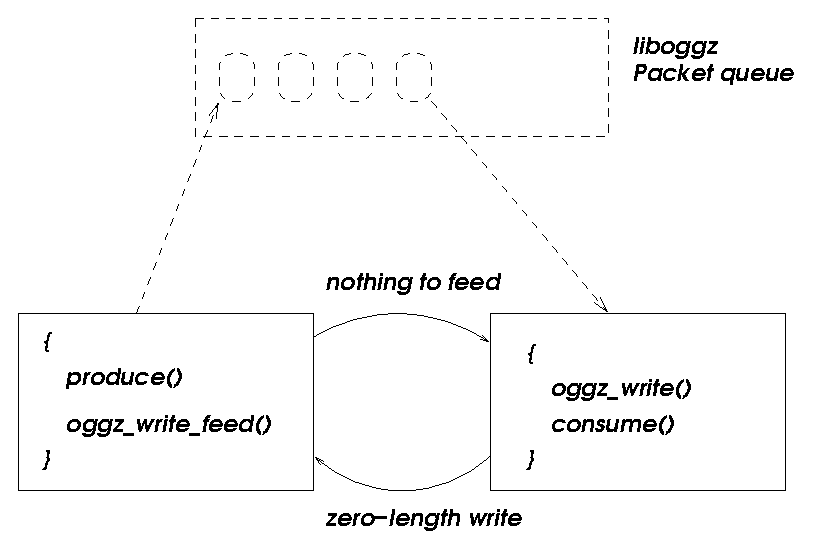
\includegraphics[width=10cm]{forcefeed}
\caption{Force Feeding Oggz}
\end{DoxyImage}


The following example code generates a stream of ten packets, each containing a single byte ('A', 'B', ... , 'J')\-:


\begin{DoxyCodeInclude}

\textcolor{preprocessor}{#include <stdlib.h>} \textcolor{comment}{/* exit */}
\textcolor{preprocessor}{#include "oggz/oggz.h"}

\textcolor{keyword}{static} \textcolor{keywordtype}{long} serialno;
\textcolor{keyword}{static} ogg\_int64\_t granulepos = 0;
\textcolor{keyword}{static} ogg\_int64\_t packetno = 0;

\textcolor{keywordtype}{int}
main (\textcolor{keywordtype}{int} argc, \textcolor{keywordtype}{char} * argv[])
\{
  \textcolor{keywordtype}{char} * progname, * filename = NULL;
  OGGZ * oggz;
  ogg\_packet op;
  \textcolor{keywordtype}{unsigned} \textcolor{keywordtype}{char} buf[1];
  \textcolor{keywordtype}{long} n;

  progname = argv[0];
  \textcolor{keywordflow}{if} (argc > 1) filename = argv[1];

  \textcolor{keywordflow}{if} (filename) \{
    oggz = oggz_open (filename, OGGZ_WRITE);
  \} \textcolor{keywordflow}{else} \{
    oggz = oggz_open_stdio (stdout, OGGZ_WRITE);
  \}

  \textcolor{keywordflow}{if} (oggz == NULL) \{
    fprintf (stderr, \textcolor{stringliteral}{"%s: Error creating oggz\(\backslash\)n"}, progname);
    exit (1);
  \}

  serialno = oggz_serialno_new (oggz);

  \textcolor{keywordflow}{for} (packetno = 0; packetno < 10; packetno++) \{

    \textcolor{comment}{/* Create a packet */}

    buf[0] = \textcolor{charliteral}{'A'} + (int)packetno;

    op.packet = buf;
    op.bytes = 1;
    op.granulepos = granulepos;
    op.packetno = packetno;
    
    \textcolor{keywordflow}{if} (packetno == 0) op.b\_o\_s = 1;
    \textcolor{keywordflow}{else} op.b\_o\_s = 0;
    
    \textcolor{keywordflow}{if} (packetno == 9) op.e\_o\_s = 1;
    \textcolor{keywordflow}{else} op.e\_o\_s = 0;
    
    \textcolor{comment}{/* Feed it to the Oggz packet queue */}

    oggz_write_feed (oggz, &op, serialno, OGGZ_FLUSH_AFTER, NULL);
    
    granulepos += 100;

    \textcolor{comment}{/* Write bytes from packetized bitstream to the output file */}

    \textcolor{keywordflow}{while} ((n = oggz_write (oggz, 32)) > 0);
  \}

  oggz_close (oggz);

  exit (0);
\}
\end{DoxyCodeInclude}
 
\section{Writing with Oggz\-Hungry callbacks}
\label{group__hungry}\index{Writing with Oggz\-Hungry callbacks@{Writing with Oggz\-Hungry callbacks}}


You can add packets to the Oggz packet queue only when it is \char`\"{}hungry\char`\"{} by providing an Oggz\-Hungry callback.  


You can add packets to the Oggz packet queue only when it is \char`\"{}hungry\char`\"{} by providing an Oggz\-Hungry callback. An Oggz\-Hungry callback will\-:
\begin{DoxyItemize}
\item Create an {\itshape ogg\-\_\-packet} structure
\item Add it to the packet queue with \doxyref{oggz\-\_\-write\-\_\-feed()}{p.}{group__write__api_ga6ccaceb107db1fd2eae047dbdbaa5889}
\end{DoxyItemize}

Once you have set such a callback with \doxyref{oggz\-\_\-write\-\_\-set\-\_\-hungry\-\_\-callback()}{p.}{group__write__api_gaf362c030bc7a7f57cb23f2b863a59389}, simply call \doxyref{oggz\-\_\-write()}{p.}{group__write__api_ga3c97d94ea425d64546adf9c368b71904} or \doxyref{oggz\-\_\-write\-\_\-output()}{p.}{group__write__api_ga5606dff01964caec4582eb172fde0c1c} repeatedly, and Oggz will call your callback to provide packets when it is hungry.

This process is illustrated in the following diagram\-:

 
\begin{DoxyImage}
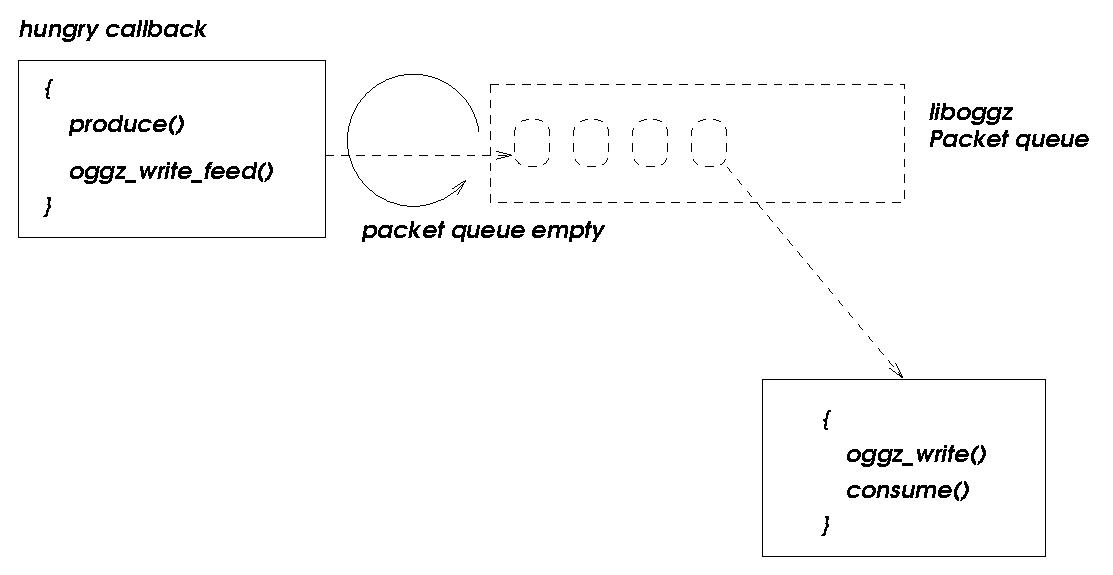
\includegraphics[width=10cm]{hungry}
\caption{Using Oggz\-Hungry}
\end{DoxyImage}


The following example code generates a stream of ten packets, each containing a single byte ('A', 'B', ... , 'J')\-:


\begin{DoxyCodeInclude}

\textcolor{preprocessor}{#include <stdlib.h>} \textcolor{comment}{/* exit */}
\textcolor{preprocessor}{#include "oggz/oggz.h"}

\textcolor{keyword}{static} \textcolor{keywordtype}{long} serialno;
\textcolor{keyword}{static} ogg\_int64\_t granulepos = 0;
\textcolor{keyword}{static} ogg\_int64\_t packetno = 0;

\textcolor{keyword}{static} \textcolor{keywordtype}{int}
hungry (OGGZ * oggz, \textcolor{keywordtype}{int} empty, \textcolor{keywordtype}{void} * user\_data)
\{
  ogg\_packet op;
  \textcolor{keywordtype}{unsigned} \textcolor{keywordtype}{char} buf[1];

  buf[0] = \textcolor{charliteral}{'A'} + (int)packetno;

  op.packet = buf;
  op.bytes = 1;
  op.granulepos = granulepos;
  op.packetno = packetno;

  \textcolor{keywordflow}{if} (packetno == 0) op.b\_o\_s = 1;
  \textcolor{keywordflow}{else} op.b\_o\_s = 0;

  \textcolor{keywordflow}{if} (packetno == 9) op.e\_o\_s = 1;
  \textcolor{keywordflow}{else} op.e\_o\_s = 0;

  oggz_write_feed (oggz, &op, serialno, OGGZ_FLUSH_AFTER, NULL);

  granulepos += 100;
  packetno++;

  \textcolor{keywordflow}{return} 0;
\}

\textcolor{keywordtype}{int}
main (\textcolor{keywordtype}{int} argc, \textcolor{keywordtype}{char} * argv[])
\{
  \textcolor{keywordtype}{char} * progname, * filename = NULL;
  OGGZ * oggz;
  \textcolor{keywordtype}{long} n;

  progname = argv[0];
  \textcolor{keywordflow}{if} (argc > 1) filename = argv[1];

  \textcolor{keywordflow}{if} (filename) \{
    oggz = oggz_open (filename, OGGZ_WRITE);
  \} \textcolor{keywordflow}{else} \{
    oggz = oggz_open_stdio (stdout, OGGZ_WRITE);
  \}

  \textcolor{keywordflow}{if} (oggz == NULL) \{
    fprintf (stderr, \textcolor{stringliteral}{"%s: Error creating oggz\(\backslash\)n"}, progname);
    exit (1);
  \}

  serialno = oggz_serialno_new (oggz);

  \textcolor{keywordflow}{if} (oggz_write_set_hungry_callback (oggz, hungry, 1, NULL) == -1) \{
    fprintf (stderr, \textcolor{stringliteral}{"%s: Error setting OggzHungry callback\(\backslash\)n"}, progname);
    exit (1);
  \}

  \textcolor{keywordflow}{while} ((n = oggz_write (oggz, 32)) > 0);

  oggz_close (oggz);

  exit (0);
\}
\end{DoxyCodeInclude}
 
\section{Oggz Write A\-P\-I}
\label{group__write__api}\index{Oggz Write A\-P\-I@{Oggz Write A\-P\-I}}


Oggz maintains a packet queue, such that you can independently add packets to the queue and write an Ogg bitstream.  


\subsection*{Typedefs}
\begin{DoxyCompactItemize}
\item 
typedef int($\ast$ {\bf Oggz\-Write\-Hungry} )({\bf O\-G\-G\-Z} $\ast$oggz, int empty, void $\ast$user\-\_\-data)
\begin{DoxyCompactList}\small\item\em This is the signature of a callback which Oggz will call when {\itshape oggz} is \doxyref{hungry }{p.}{group__hungry}. \end{DoxyCompactList}\end{DoxyCompactItemize}
\subsection*{Functions}
\begin{DoxyCompactItemize}
\item 
int {\bf oggz\-\_\-write\-\_\-set\-\_\-hungry\-\_\-callback} ({\bf O\-G\-G\-Z} $\ast$oggz, {\bf Oggz\-Write\-Hungry} hungry, int only\-\_\-when\-\_\-empty, void $\ast$user\-\_\-data)
\begin{DoxyCompactList}\small\item\em Set a callback for Oggz to call when {\itshape oggz} is \doxyref{hungry }{p.}{group__hungry}. \end{DoxyCompactList}\item 
int {\bf oggz\-\_\-write\-\_\-feed} ({\bf O\-G\-G\-Z} $\ast$oggz, ogg\-\_\-packet $\ast$op, long serialno, int flush, int $\ast$guard)
\begin{DoxyCompactList}\small\item\em Add a packet to {\itshape oggz's} packet queue. \end{DoxyCompactList}\item 
long {\bf oggz\-\_\-write\-\_\-output} ({\bf O\-G\-G\-Z} $\ast$oggz, unsigned char $\ast$buf, long n)
\begin{DoxyCompactList}\small\item\em Output data from an O\-G\-G\-Z handle. \end{DoxyCompactList}\item 
long {\bf oggz\-\_\-write} ({\bf O\-G\-G\-Z} $\ast$oggz, long n)
\begin{DoxyCompactList}\small\item\em Write n bytes from an O\-G\-G\-Z handle. \end{DoxyCompactList}\item 
long {\bf oggz\-\_\-write\-\_\-get\-\_\-next\-\_\-page\-\_\-size} ({\bf O\-G\-G\-Z} $\ast$oggz)
\begin{DoxyCompactList}\small\item\em Query the number of bytes in the next page to be written. \end{DoxyCompactList}\end{DoxyCompactItemize}


\subsection{Detailed Description}
Oggz maintains a packet queue, such that you can independently add packets to the queue and write an Ogg bitstream. There are two complementary methods for adding packets to the packet queue.


\begin{DoxyItemize}
\item by \doxyref{force feeding Oggz }{p.}{group__force__feed}
\item by using \doxyref{Oggz\-Hungry }{p.}{group__hungry} callbacks
\end{DoxyItemize}

As each packet is enqueued, its validity is checked against the framing constraints outlined in the \doxyref{Ogg basics }{p.}{group__basics} section. If it does not pass these constraints, \doxyref{oggz\-\_\-write\-\_\-feed()}{p.}{group__write__api_ga6ccaceb107db1fd2eae047dbdbaa5889} will fail with an appropriate error code.

\begin{DoxyNote}{Note}

\begin{DoxyItemize}
\item When writing, you can ensure that a packet starts on a new page by setting the {\itshape flush} parameter of \doxyref{oggz\-\_\-write\-\_\-feed()}{p.}{group__write__api_ga6ccaceb107db1fd2eae047dbdbaa5889} to {\itshape O\-G\-G\-Z\-\_\-\-F\-L\-U\-S\-H\-\_\-\-B\-E\-F\-O\-R\-E} when enqueuing it. Similarly you can ensure that the last page a packet is written into won't contain any following packets by setting the {\itshape flush} parameter of \doxyref{oggz\-\_\-write\-\_\-feed()}{p.}{group__write__api_ga6ccaceb107db1fd2eae047dbdbaa5889} to {\itshape O\-G\-G\-Z\-\_\-\-F\-L\-U\-S\-H\-\_\-\-A\-F\-T\-E\-R}.
\item The {\itshape O\-G\-G\-Z\-\_\-\-F\-L\-U\-S\-H\-\_\-\-B\-E\-F\-O\-R\-E} and {\itshape O\-G\-G\-Z\-\_\-\-F\-L\-U\-S\-H\-\_\-\-A\-F\-T\-E\-R} flags can be bitwise O\-R'd together to ensure that the packet will not share any pages with any other packets, either before or after. 
\end{DoxyItemize}
\end{DoxyNote}


\subsection{Typedef Documentation}
\index{Oggz Write A\-P\-I@{Oggz Write A\-P\-I}!Oggz\-Write\-Hungry@{Oggz\-Write\-Hungry}}
\index{Oggz\-Write\-Hungry@{Oggz\-Write\-Hungry}!Oggz Write API@{Oggz Write A\-P\-I}}
\subsubsection[{Oggz\-Write\-Hungry}]{\setlength{\rightskip}{0pt plus 5cm}typedef int($\ast$ Oggz\-Write\-Hungry)({\bf O\-G\-G\-Z} $\ast$oggz, int empty, void $\ast$user\-\_\-data)}\label{group__write__api_ga27ef9f56078d3c015431b1a67b2c1812}


This is the signature of a callback which Oggz will call when {\itshape oggz} is \doxyref{hungry }{p.}{group__hungry}. 


\begin{DoxyParams}{Parameters}
{\em oggz} & The O\-G\-G\-Z handle \\
\hline
{\em empty} & A value of 1 indicates that the packet queue is currently empty. A value of 0 indicates that the packet queue is not empty. \\
\hline
{\em user\-\_\-data} & A generic pointer you have provided earlier \\
\hline
\end{DoxyParams}

\begin{DoxyRetVals}{Return values}
{\em 0} & Continue \\
\hline
{\em non-\/zero} & Instruct Oggz to stop. \\
\hline
\end{DoxyRetVals}


\subsection{Function Documentation}
\index{Oggz Write A\-P\-I@{Oggz Write A\-P\-I}!oggz\-\_\-write@{oggz\-\_\-write}}
\index{oggz\-\_\-write@{oggz\-\_\-write}!Oggz Write API@{Oggz Write A\-P\-I}}
\subsubsection[{oggz\-\_\-write}]{\setlength{\rightskip}{0pt plus 5cm}long oggz\-\_\-write (
\begin{DoxyParamCaption}
\item[{{\bf O\-G\-G\-Z} $\ast$}]{oggz, }
\item[{long}]{n}
\end{DoxyParamCaption}
)}\label{group__write__api_ga3c97d94ea425d64546adf9c368b71904}


Write n bytes from an O\-G\-G\-Z handle. 

Oggz will call your write callback as needed.


\begin{DoxyParams}{Parameters}
{\em oggz} & An O\-G\-G\-Z handle previously opened for writing \\
\hline
{\em n} & A count of bytes to be written \\
\hline
\end{DoxyParams}

\begin{DoxyRetVals}{Return values}
{\em $>$ 0} & The number of bytes successfully output \\
\hline
{\em 0} & End of stream \\
\hline
{\em O\-G\-G\-Z\-\_\-\-E\-R\-R\-\_\-\-R\-E\-C\-U\-R\-S\-I\-V\-E\-\_\-\-W\-R\-I\-T\-E} & Attempt to initiate writing from within an Oggz\-Hungry callback \\
\hline
{\em O\-G\-G\-Z\-\_\-\-E\-R\-R\-\_\-\-B\-A\-D\-\_\-\-O\-G\-G\-Z} & {\itshape oggz} does not refer to an existing O\-G\-G\-Z \\
\hline
{\em O\-G\-G\-Z\-\_\-\-E\-R\-R\-\_\-\-I\-N\-V\-A\-L\-I\-D} & Operation not suitable for this O\-G\-G\-Z \\
\hline
{\em O\-G\-G\-Z\-\_\-\-E\-R\-R\-\_\-\-S\-T\-O\-P\-\_\-\-O\-K} & Writing was stopped by an Oggz\-Hungry callback returning O\-G\-G\-Z\-\_\-\-S\-T\-O\-P\-\_\-\-O\-K \\
\hline
{\em O\-G\-G\-Z\-\_\-\-E\-R\-R\-\_\-\-S\-T\-O\-P\-\_\-\-E\-R\-R} & Reading was stopped by an Oggz\-Hungry callback returning O\-G\-G\-Z\-\_\-\-S\-T\-O\-P\-\_\-\-E\-R\-R \\
\hline
\end{DoxyRetVals}
\index{Oggz Write A\-P\-I@{Oggz Write A\-P\-I}!oggz\-\_\-write\-\_\-feed@{oggz\-\_\-write\-\_\-feed}}
\index{oggz\-\_\-write\-\_\-feed@{oggz\-\_\-write\-\_\-feed}!Oggz Write API@{Oggz Write A\-P\-I}}
\subsubsection[{oggz\-\_\-write\-\_\-feed}]{\setlength{\rightskip}{0pt plus 5cm}int oggz\-\_\-write\-\_\-feed (
\begin{DoxyParamCaption}
\item[{{\bf O\-G\-G\-Z} $\ast$}]{oggz, }
\item[{ogg\-\_\-packet $\ast$}]{op, }
\item[{long}]{serialno, }
\item[{int}]{flush, }
\item[{int $\ast$}]{guard}
\end{DoxyParamCaption}
)}\label{group__write__api_ga6ccaceb107db1fd2eae047dbdbaa5889}


Add a packet to {\itshape oggz's} packet queue. 


\begin{DoxyParams}{Parameters}
{\em oggz} & An O\-G\-G\-Z handle previously opened for writing \\
\hline
{\em op} & An ogg\-\_\-packet with all fields filled in \\
\hline
{\em serialno} & Identify the logical bitstream in {\itshape oggz} to add the packet to \\
\hline
{\em flush} & Bitmask of O\-G\-G\-Z\-\_\-\-F\-L\-U\-S\-H\-\_\-\-B\-E\-F\-O\-R\-E, O\-G\-G\-Z\-\_\-\-F\-L\-U\-S\-H\-\_\-\-A\-F\-T\-E\-R \\
\hline
{\em guard} & A guard for nocopy, N\-U\-L\-L otherwise \\
\hline
\end{DoxyParams}

\begin{DoxyRetVals}{Return values}
{\em 0} & Success \\
\hline
{\em O\-G\-G\-Z\-\_\-\-E\-R\-R\-\_\-\-B\-A\-D\-\_\-\-G\-U\-A\-R\-D} & {\itshape guard} specified has non-\/zero initialization \\
\hline
{\em O\-G\-G\-Z\-\_\-\-E\-R\-R\-\_\-\-B\-O\-S} & Packet would be bos packet of a new logical bitstream, but oggz has already written one or more non-\/bos packets in other logical bitstreams, and {\itshape oggz} is not flagged O\-G\-G\-Z\-\_\-\-N\-O\-N\-S\-T\-R\-I\-C\-T \\
\hline
{\em O\-G\-G\-Z\-\_\-\-E\-R\-R\-\_\-\-E\-O\-S} & The logical bitstream identified by {\itshape serialno} is already at eos, and {\itshape oggz} is not flagged O\-G\-G\-Z\-\_\-\-N\-O\-N\-S\-T\-R\-I\-C\-T \\
\hline
{\em O\-G\-G\-Z\-\_\-\-E\-R\-R\-\_\-\-B\-A\-D\-\_\-\-B\-Y\-T\-E\-S} & {\itshape op-\/$>$bytes} is invalid, and {\itshape oggz} is not flagged O\-G\-G\-Z\-\_\-\-N\-O\-N\-S\-T\-R\-I\-C\-T \\
\hline
{\em O\-G\-G\-Z\-\_\-\-E\-R\-R\-\_\-\-B\-A\-D\-\_\-\-B\-\_\-\-O\-\_\-\-S} & {\itshape op-\/$>$b\-\_\-o\-\_\-s} is invalid, and {\itshape oggz} is not flagged O\-G\-G\-Z\-\_\-\-N\-O\-N\-S\-T\-R\-I\-C\-T \\
\hline
{\em O\-G\-G\-Z\-\_\-\-E\-R\-R\-\_\-\-B\-A\-D\-\_\-\-G\-R\-A\-N\-U\-L\-E\-P\-O\-S} & {\itshape op-\/$>$granulepos} is less than that of an earlier packet within this logical bitstream, and {\itshape oggz} is not flagged O\-G\-G\-Z\-\_\-\-N\-O\-N\-S\-T\-R\-I\-C\-T \\
\hline
{\em O\-G\-G\-Z\-\_\-\-E\-R\-R\-\_\-\-B\-A\-D\-\_\-\-P\-A\-C\-K\-E\-T\-N\-O} & {\itshape op-\/$>$packetno} is less than that of an earlier packet within this logical bitstream, and {\itshape oggz} is not flagged O\-G\-G\-Z\-\_\-\-N\-O\-N\-S\-T\-R\-I\-C\-T \\
\hline
{\em O\-G\-G\-Z\-\_\-\-E\-R\-R\-\_\-\-B\-A\-D\-\_\-\-S\-E\-R\-I\-A\-L\-N\-O} & {\itshape serialno} does not identify an existing logical bitstream in {\itshape oggz}, and {\itshape oggz} is not flagged O\-G\-G\-Z\-\_\-\-N\-O\-N\-S\-T\-R\-I\-C\-T or {\itshape serialno} is equal to -\/1, or {\itshape serialno} does not fit in 32 bits, ie. within the range (-\/(2$^\wedge$31), (2$^\wedge$31)-\/1) \\
\hline
{\em O\-G\-G\-Z\-\_\-\-E\-R\-R\-\_\-\-B\-A\-D\-\_\-\-O\-G\-G\-Z} & {\itshape oggz} does not refer to an existing O\-G\-G\-Z \\
\hline
{\em O\-G\-G\-Z\-\_\-\-E\-R\-R\-\_\-\-I\-N\-V\-A\-L\-I\-D} & Operation not suitable for this O\-G\-G\-Z \\
\hline
{\em O\-G\-G\-Z\-\_\-\-E\-R\-R\-\_\-\-O\-U\-T\-\_\-\-O\-F\-\_\-\-M\-E\-M\-O\-R\-Y} & Unable to allocate memory to queue packet\\
\hline
\end{DoxyRetVals}
\begin{DoxyNote}{Note}
If {\itshape op-\/$>$b\-\_\-o\-\_\-s} is initialized to {\itshape -\/1} before calling \doxyref{oggz\-\_\-write\-\_\-feed()}{p.}{group__write__api_ga6ccaceb107db1fd2eae047dbdbaa5889}, Oggz will fill it in with the appropriate value; ie. 1 for the first packet of a new stream, and 0 otherwise. 
\end{DoxyNote}
\index{Oggz Write A\-P\-I@{Oggz Write A\-P\-I}!oggz\-\_\-write\-\_\-get\-\_\-next\-\_\-page\-\_\-size@{oggz\-\_\-write\-\_\-get\-\_\-next\-\_\-page\-\_\-size}}
\index{oggz\-\_\-write\-\_\-get\-\_\-next\-\_\-page\-\_\-size@{oggz\-\_\-write\-\_\-get\-\_\-next\-\_\-page\-\_\-size}!Oggz Write API@{Oggz Write A\-P\-I}}
\subsubsection[{oggz\-\_\-write\-\_\-get\-\_\-next\-\_\-page\-\_\-size}]{\setlength{\rightskip}{0pt plus 5cm}long oggz\-\_\-write\-\_\-get\-\_\-next\-\_\-page\-\_\-size (
\begin{DoxyParamCaption}
\item[{{\bf O\-G\-G\-Z} $\ast$}]{oggz}
\end{DoxyParamCaption}
)}\label{group__write__api_gab25da7d2cbf39585357f2a426d3dba2f}


Query the number of bytes in the next page to be written. 


\begin{DoxyParams}{Parameters}
{\em oggz} & An O\-G\-G\-Z handle previously opened for writing \\
\hline
\end{DoxyParams}

\begin{DoxyRetVals}{Return values}
{\em $>$= 0} & The number of bytes in the next page \\
\hline
{\em O\-G\-G\-Z\-\_\-\-E\-R\-R\-\_\-\-B\-A\-D\-\_\-\-O\-G\-G\-Z} & {\itshape oggz} does not refer to an existing O\-G\-G\-Z \\
\hline
{\em O\-G\-G\-Z\-\_\-\-E\-R\-R\-\_\-\-I\-N\-V\-A\-L\-I\-D} & Operation not suitable for this O\-G\-G\-Z \\
\hline
\end{DoxyRetVals}
\index{Oggz Write A\-P\-I@{Oggz Write A\-P\-I}!oggz\-\_\-write\-\_\-output@{oggz\-\_\-write\-\_\-output}}
\index{oggz\-\_\-write\-\_\-output@{oggz\-\_\-write\-\_\-output}!Oggz Write API@{Oggz Write A\-P\-I}}
\subsubsection[{oggz\-\_\-write\-\_\-output}]{\setlength{\rightskip}{0pt plus 5cm}long oggz\-\_\-write\-\_\-output (
\begin{DoxyParamCaption}
\item[{{\bf O\-G\-G\-Z} $\ast$}]{oggz, }
\item[{unsigned char $\ast$}]{buf, }
\item[{long}]{n}
\end{DoxyParamCaption}
)}\label{group__write__api_ga5606dff01964caec4582eb172fde0c1c}


Output data from an O\-G\-G\-Z handle. 

Oggz will call your write callback as needed.


\begin{DoxyParams}{Parameters}
{\em oggz} & An O\-G\-G\-Z handle previously opened for writing \\
\hline
{\em buf} & A memory buffer \\
\hline
{\em n} & A count of bytes to output \\
\hline
\end{DoxyParams}

\begin{DoxyRetVals}{Return values}
{\em $>$ 0} & The number of bytes successfully output \\
\hline
{\em 0} & End of stream \\
\hline
{\em O\-G\-G\-Z\-\_\-\-E\-R\-R\-\_\-\-R\-E\-C\-U\-R\-S\-I\-V\-E\-\_\-\-W\-R\-I\-T\-E} & Attempt to initiate writing from within an Oggz\-Hungry callback \\
\hline
{\em O\-G\-G\-Z\-\_\-\-E\-R\-R\-\_\-\-B\-A\-D\-\_\-\-O\-G\-G\-Z} & {\itshape oggz} does not refer to an existing O\-G\-G\-Z \\
\hline
{\em O\-G\-G\-Z\-\_\-\-E\-R\-R\-\_\-\-I\-N\-V\-A\-L\-I\-D} & Operation not suitable for this O\-G\-G\-Z \\
\hline
{\em O\-G\-G\-Z\-\_\-\-E\-R\-R\-\_\-\-S\-T\-O\-P\-\_\-\-O\-K} & Writing was stopped by an Oggz\-Hungry callback returning O\-G\-G\-Z\-\_\-\-S\-T\-O\-P\-\_\-\-O\-K \\
\hline
{\em O\-G\-G\-Z\-\_\-\-E\-R\-R\-\_\-\-S\-T\-O\-P\-\_\-\-E\-R\-R} & Reading was stopped by an Oggz\-Hungry callback returning O\-G\-G\-Z\-\_\-\-S\-T\-O\-P\-\_\-\-E\-R\-R \\
\hline
\end{DoxyRetVals}
\index{Oggz Write A\-P\-I@{Oggz Write A\-P\-I}!oggz\-\_\-write\-\_\-set\-\_\-hungry\-\_\-callback@{oggz\-\_\-write\-\_\-set\-\_\-hungry\-\_\-callback}}
\index{oggz\-\_\-write\-\_\-set\-\_\-hungry\-\_\-callback@{oggz\-\_\-write\-\_\-set\-\_\-hungry\-\_\-callback}!Oggz Write API@{Oggz Write A\-P\-I}}
\subsubsection[{oggz\-\_\-write\-\_\-set\-\_\-hungry\-\_\-callback}]{\setlength{\rightskip}{0pt plus 5cm}int oggz\-\_\-write\-\_\-set\-\_\-hungry\-\_\-callback (
\begin{DoxyParamCaption}
\item[{{\bf O\-G\-G\-Z} $\ast$}]{oggz, }
\item[{{\bf Oggz\-Write\-Hungry}}]{hungry, }
\item[{int}]{only\-\_\-when\-\_\-empty, }
\item[{void $\ast$}]{user\-\_\-data}
\end{DoxyParamCaption}
)}\label{group__write__api_gaf362c030bc7a7f57cb23f2b863a59389}


Set a callback for Oggz to call when {\itshape oggz} is \doxyref{hungry }{p.}{group__hungry}. 


\begin{DoxyParams}{Parameters}
{\em oggz} & An O\-G\-G\-Z handle previously opened for writing \\
\hline
{\em hungry} & Your callback function \\
\hline
{\em only\-\_\-when\-\_\-empty} & When to call\-: a value of 0 indicates that Oggz should call {\itshape hungry()} after each and every packet is written; a value of 1 indicates that Oggz should call {\itshape hungry()} only when its packet queue is empty \\
\hline
{\em user\-\_\-data} & Arbitrary data you wish to pass to your callback \\
\hline
\end{DoxyParams}

\begin{DoxyRetVals}{Return values}
{\em 0} & Success \\
\hline
{\em O\-G\-G\-Z\-\_\-\-E\-R\-R\-\_\-\-B\-A\-D\-\_\-\-O\-G\-G\-Z} & {\itshape oggz} does not refer to an existing O\-G\-G\-Z \\
\hline
{\em O\-G\-G\-Z\-\_\-\-E\-R\-R\-\_\-\-I\-N\-V\-A\-L\-I\-D} & Operation not suitable for this O\-G\-G\-Z \\
\hline
\end{DoxyRetVals}
\begin{DoxyNote}{Note}
Passing a value of 0 for {\itshape only\-\_\-when\-\_\-empty} allows you to feed new packets into {\itshape oggz's} packet queue on the fly. 
\end{DoxyNote}

\chapter{Data Structure Documentation}
\section{oggz\-\_\-packet Struct Reference}
\label{structoggz__packet}\index{oggz\-\_\-packet@{oggz\-\_\-packet}}


An ogg\-\_\-packet and its position in the stream.  




{\ttfamily \#include $<$oggz\-\_\-packet.\-h$>$}

\subsection*{Data Fields}
\begin{DoxyCompactItemize}
\item 
ogg\-\_\-packet {\bf op}\label{structoggz__packet_a36cb056219e68a383e7139ce0a2ff715}

\begin{DoxyCompactList}\small\item\em The ogg\-\_\-packet structure, defined in $<$ogg/ogg.\-h$>$ \end{DoxyCompactList}\item 
{\bf oggz\-\_\-position} {\bf pos}\label{structoggz__packet_a71d24b8fa94acf2511c0c6f7b24de546}

\begin{DoxyCompactList}\small\item\em Its position. \end{DoxyCompactList}\end{DoxyCompactItemize}


\subsection{Detailed Description}
An ogg\-\_\-packet and its position in the stream. 

The documentation for this struct was generated from the following file\-:\begin{DoxyCompactItemize}
\item 
{\bf oggz\-\_\-packet.\-h}\end{DoxyCompactItemize}

\section{oggz\-\_\-position Struct Reference}
\label{structoggz__position}\index{oggz\-\_\-position@{oggz\-\_\-position}}


The position of an \doxyref{oggz\-\_\-packet}{p.}{structoggz__packet}.  




{\ttfamily \#include $<$oggz\-\_\-packet.\-h$>$}

\subsection*{Data Fields}
\begin{DoxyCompactItemize}
\item 
ogg\-\_\-int64\-\_\-t {\bf calc\-\_\-granulepos}
\begin{DoxyCompactList}\small\item\em Granulepos calculated by inspection of codec data. \end{DoxyCompactList}\item 
{\bf oggz\-\_\-off\-\_\-t} {\bf begin\-\_\-page\-\_\-offset}\label{structoggz__position_ae9c2a34bd23aea39a2136415b2666487}

\begin{DoxyCompactList}\small\item\em Byte offset of the start of the page on which this packet begins. \end{DoxyCompactList}\item 
{\bf oggz\-\_\-off\-\_\-t} {\bf end\-\_\-page\-\_\-offset}\label{structoggz__position_a7130786ffc28acab7c3a9a77c7cfbbb6}

\begin{DoxyCompactList}\small\item\em Byte offset of the start of the page on which this packet ends. \end{DoxyCompactList}\item 
int {\bf pages}
\begin{DoxyCompactList}\small\item\em Number of pages this packet spans. \end{DoxyCompactList}\item 
int {\bf begin\-\_\-segment\-\_\-index}
\begin{DoxyCompactList}\small\item\em Index into begin\-\_\-page's lacing values for the segment that begins this packet. \end{DoxyCompactList}\end{DoxyCompactItemize}


\subsection{Detailed Description}
The position of an \doxyref{oggz\-\_\-packet}{p.}{structoggz__packet}. 

\subsection{Field Documentation}
\index{oggz\-\_\-position@{oggz\-\_\-position}!begin\-\_\-segment\-\_\-index@{begin\-\_\-segment\-\_\-index}}
\index{begin\-\_\-segment\-\_\-index@{begin\-\_\-segment\-\_\-index}!oggz_position@{oggz\-\_\-position}}
\subsubsection[{begin\-\_\-segment\-\_\-index}]{\setlength{\rightskip}{0pt plus 5cm}int oggz\-\_\-position\-::begin\-\_\-segment\-\_\-index}\label{structoggz__position_a8ca77b0acf589531d9970c3f6b589164}


Index into begin\-\_\-page's lacing values for the segment that begins this packet. 

N\-B. if begin\-\_\-page is continued then the first of these packets will not be reported by ogg\-\_\-sync\-\_\-packetout() after a seek. -\/1 if unknown. \index{oggz\-\_\-position@{oggz\-\_\-position}!calc\-\_\-granulepos@{calc\-\_\-granulepos}}
\index{calc\-\_\-granulepos@{calc\-\_\-granulepos}!oggz_position@{oggz\-\_\-position}}
\subsubsection[{calc\-\_\-granulepos}]{\setlength{\rightskip}{0pt plus 5cm}ogg\-\_\-int64\-\_\-t oggz\-\_\-position\-::calc\-\_\-granulepos}\label{structoggz__position_af7eb619f0da5c818b49cbabc29c540b4}


Granulepos calculated by inspection of codec data. 

-\/1 if unknown \index{oggz\-\_\-position@{oggz\-\_\-position}!pages@{pages}}
\index{pages@{pages}!oggz_position@{oggz\-\_\-position}}
\subsubsection[{pages}]{\setlength{\rightskip}{0pt plus 5cm}int oggz\-\_\-position\-::pages}\label{structoggz__position_ad2e55a8276c03f83c6e40b88991305b2}


Number of pages this packet spans. 



The documentation for this struct was generated from the following file\-:\begin{DoxyCompactItemize}
\item 
{\bf oggz\-\_\-packet.\-h}\end{DoxyCompactItemize}

\section{Oggz\-Comment Struct Reference}
\label{structOggzComment}\index{Oggz\-Comment@{Oggz\-Comment}}


A comment.  




{\ttfamily \#include $<$oggz\-\_\-comments.\-h$>$}

\subsection*{Data Fields}
\begin{DoxyCompactItemize}
\item 
char $\ast$ {\bf name}
\begin{DoxyCompactList}\small\item\em The name of the comment, eg. \end{DoxyCompactList}\item 
char $\ast$ {\bf value}\label{structOggzComment_ae300da8b29b69ea083b47035e944f9bb}

\begin{DoxyCompactList}\small\item\em The value of the comment, as U\-T\-F-\/8. \end{DoxyCompactList}\end{DoxyCompactItemize}


\subsection{Detailed Description}
A comment. 

\subsection{Field Documentation}
\index{Oggz\-Comment@{Oggz\-Comment}!name@{name}}
\index{name@{name}!OggzComment@{Oggz\-Comment}}
\subsubsection[{name}]{\setlength{\rightskip}{0pt plus 5cm}char$\ast$ Oggz\-Comment\-::name}\label{structOggzComment_af1b4e3c3e42e17054b6164bbdee5a37f}


The name of the comment, eg. 

\char`\"{}\-A\-U\-T\-H\-O\-R\char`\"{} 

The documentation for this struct was generated from the following file\-:\begin{DoxyCompactItemize}
\item 
{\bf oggz\-\_\-comments.\-h}\end{DoxyCompactItemize}

\chapter{File Documentation}
\section{oggz.\-h File Reference}
\label{oggz_8h}\index{oggz.\-h@{oggz.\-h}}


The liboggz C A\-P\-I.  


{\ttfamily \#include $<$stdio.\-h$>$}\\*
{\ttfamily \#include $<$sys/types.\-h$>$}\\*
{\ttfamily \#include $<$ogg/ogg.\-h$>$}\\*
{\ttfamily \#include $<$oggz/oggz\-\_\-constants.\-h$>$}\\*
{\ttfamily \#include $<$oggz/oggz\-\_\-table.\-h$>$}\\*
{\ttfamily \#include $<$oggz/oggz\-\_\-off\-\_\-t.\-h$>$}\\*
{\ttfamily \#include $<$oggz/oggz\-\_\-read.\-h$>$}\\*
{\ttfamily \#include $<$oggz/oggz\-\_\-stream.\-h$>$}\\*
{\ttfamily \#include $<$oggz/oggz\-\_\-seek.\-h$>$}\\*
{\ttfamily \#include $<$oggz/oggz\-\_\-write.\-h$>$}\\*
{\ttfamily \#include $<$oggz/oggz\-\_\-io.\-h$>$}\\*
{\ttfamily \#include $<$oggz/oggz\-\_\-comments.\-h$>$}\\*
{\ttfamily \#include $<$oggz/oggz\-\_\-deprecated.\-h$>$}\\*
\subsection*{Typedefs}
\begin{DoxyCompactItemize}
\item 
typedef void {\bf O\-G\-G\-Z}
\begin{DoxyCompactList}\small\item\em An opaque handle to an Ogg file. \end{DoxyCompactList}\end{DoxyCompactItemize}
\subsection*{Functions}
\begin{DoxyCompactItemize}
\item 
{\bf O\-G\-G\-Z} $\ast$ {\bf oggz\-\_\-new} (int flags)
\begin{DoxyCompactList}\small\item\em Create a new O\-G\-G\-Z object. \end{DoxyCompactList}\item 
{\bf O\-G\-G\-Z} $\ast$ {\bf oggz\-\_\-open} (const char $\ast$filename, int flags)
\begin{DoxyCompactList}\small\item\em Open an Ogg file, creating an O\-G\-G\-Z handle for it. \end{DoxyCompactList}\item 
{\bf O\-G\-G\-Z} $\ast$ {\bf oggz\-\_\-open\-\_\-stdio} (F\-I\-L\-E $\ast$file, int flags)
\begin{DoxyCompactList}\small\item\em Create an O\-G\-G\-Z handle associated with a stdio stream. \end{DoxyCompactList}\item 
int {\bf oggz\-\_\-flush} ({\bf O\-G\-G\-Z} $\ast$oggz)
\begin{DoxyCompactList}\small\item\em Ensure any associated io streams are flushed. \end{DoxyCompactList}\item 
long {\bf oggz\-\_\-run} ({\bf O\-G\-G\-Z} $\ast$oggz)
\begin{DoxyCompactList}\small\item\em Run an O\-G\-G\-Z until completion, or error. \end{DoxyCompactList}\item 
int {\bf oggz\-\_\-run\-\_\-set\-\_\-blocksize} ({\bf O\-G\-G\-Z} $\ast$oggz, long blocksize)
\begin{DoxyCompactList}\small\item\em Set the blocksize to use internally for \doxyref{oggz\-\_\-run()}{p.}{oggz_8h_a0561df532fc37f98725007a79f898356} \end{DoxyCompactList}\item 
int {\bf oggz\-\_\-close} ({\bf O\-G\-G\-Z} $\ast$oggz)
\begin{DoxyCompactList}\small\item\em Close an O\-G\-G\-Z handle. \end{DoxyCompactList}\item 
int {\bf oggz\-\_\-get\-\_\-bos} ({\bf O\-G\-G\-Z} $\ast$oggz, long serialno)
\begin{DoxyCompactList}\small\item\em Determine if a given logical bitstream is at bos (beginning of stream). \end{DoxyCompactList}\item 
int {\bf oggz\-\_\-get\-\_\-eos} ({\bf O\-G\-G\-Z} $\ast$oggz, long serialno)
\begin{DoxyCompactList}\small\item\em Determine if a given logical bitstream is at eos (end of stream). \end{DoxyCompactList}\item 
int {\bf oggz\-\_\-get\-\_\-numtracks} ({\bf O\-G\-G\-Z} $\ast$oggz)
\begin{DoxyCompactList}\small\item\em Query the number of tracks (logical bitstreams). \end{DoxyCompactList}\item 
long {\bf oggz\-\_\-serialno\-\_\-new} ({\bf O\-G\-G\-Z} $\ast$oggz)
\begin{DoxyCompactList}\small\item\em Request a new serialno, as required for a new stream, ensuring the serialno is not yet used for any other streams managed by this O\-G\-G\-Z. \end{DoxyCompactList}\item 
const char $\ast$ {\bf oggz\-\_\-content\-\_\-type} ({\bf Oggz\-Stream\-Content} content)
\begin{DoxyCompactList}\small\item\em Return human-\/readable string representation of a content type. \end{DoxyCompactList}\end{DoxyCompactItemize}


\subsection{Detailed Description}
The liboggz C A\-P\-I. \subsection{Generic semantics}\label{oggz_8h_general}
All access is managed via an O\-G\-G\-Z handle. This can be instantiated in one of three ways\-:


\begin{DoxyItemize}
\item \doxyref{oggz\-\_\-open()}{p.}{oggz_8h_a65197cdd03f755f7ebfabf2fdff4c7db} -\/ Open a full pathname
\item \doxyref{oggz\-\_\-open\-\_\-stdio()}{p.}{oggz_8h_ac49e9de0bc4ef1d91b43b13605f98b19} -\/ Use an already opened F\-I\-L\-E $\ast$
\item \doxyref{oggz\-\_\-new()}{p.}{oggz_8h_a6eb34d123389ae38d993601f9e7bb9d6} -\/ Create an anonymous O\-G\-G\-Z object, which you can later handle via memory buffers
\end{DoxyItemize}

To finish using an O\-G\-G\-Z handle, it should be closed with \doxyref{oggz\-\_\-close()}{p.}{oggz_8h_aadcfc04b2930660710bbcbc93140b783}.\subsection{Reading Ogg data}\label{oggz_8h_reading}
To read from Ogg files or streams you must instantiate an O\-G\-G\-Z handle with flags set to O\-G\-G\-Z\-\_\-\-R\-E\-A\-D, and provide an Oggz\-Read\-Packet callback with \doxyref{oggz\-\_\-set\-\_\-read\-\_\-callback()}{p.}{group__read__api_ga6d5aae4f7f186fffe19d4fd3cd63148d}. See the \doxyref{Oggz Read A\-P\-I}{p.}{group__read__api} section for details.\subsection{Writing Ogg data}\label{oggz_8h_writing}
To write to Ogg files or streams you must instantiate an O\-G\-G\-Z handle with flags set to O\-G\-G\-Z\-\_\-\-W\-R\-I\-T\-E, and provide an Oggz\-Write\-Packet callback with oggz\-\_\-set\-\_\-write\-\_\-callback(). See the \doxyref{Oggz Write A\-P\-I}{p.}{group__write__api} section for details.\subsection{Seeking on Ogg data}\label{oggz_8h_seeking}
To seek while reading Ogg files or streams you must instantiate an O\-G\-G\-Z handle for reading, and ensure that an \doxyref{Oggz\-Metric }{p.}{group__metric} function is defined to translate packet positions into units such as time. See the \doxyref{Oggz Seek A\-P\-I}{p.}{group__seek__api} section for details.\subsection{Overriding the I\-O methods}\label{oggz_8h_io}
When an O\-G\-G\-Z handle is instantiated by \doxyref{oggz\-\_\-open()}{p.}{oggz_8h_a65197cdd03f755f7ebfabf2fdff4c7db} or \doxyref{oggz\-\_\-open\-\_\-stdio()}{p.}{oggz_8h_ac49e9de0bc4ef1d91b43b13605f98b19}, Oggz uses stdio functions internally to access the raw data. However for some applications, the raw data cannot be accessed via stdio -- this commonly occurs when integrating with media frameworks. For such applications, you can provide Oggz with custom I\-O methods that it should use to access the raw data. Oggz will then use these custom methods, rather than using stdio methods, to access the raw data internally.

For details, see \doxyref{$<$oggz/oggz\-\_\-io.\-h$>$ }{p.}{oggz__io_8h}.\subsection{Headers}\label{oggz_8h_headers}
\doxyref{oggz.\-h}{p.}{oggz_8h} provides direct access to libogg types such as ogg\-\_\-packet, defined in $<$ogg/ogg.\-h$>$. 

\subsection{Typedef Documentation}
\index{oggz.\-h@{oggz.\-h}!O\-G\-G\-Z@{O\-G\-G\-Z}}
\index{O\-G\-G\-Z@{O\-G\-G\-Z}!oggz.h@{oggz.\-h}}
\subsubsection[{O\-G\-G\-Z}]{\setlength{\rightskip}{0pt plus 5cm}typedef void {\bf O\-G\-G\-Z}}\label{oggz_8h_a672d218df13da45a4b41d5366211bfee}


An opaque handle to an Ogg file. 

This is returned by \doxyref{oggz\-\_\-open()}{p.}{oggz_8h_a65197cdd03f755f7ebfabf2fdff4c7db} or \doxyref{oggz\-\_\-new()}{p.}{oggz_8h_a6eb34d123389ae38d993601f9e7bb9d6}, and is passed to all other oggz\-\_\-$\ast$ functions. 

\subsection{Function Documentation}
\index{oggz.\-h@{oggz.\-h}!oggz\-\_\-close@{oggz\-\_\-close}}
\index{oggz\-\_\-close@{oggz\-\_\-close}!oggz.h@{oggz.\-h}}
\subsubsection[{oggz\-\_\-close}]{\setlength{\rightskip}{0pt plus 5cm}int oggz\-\_\-close (
\begin{DoxyParamCaption}
\item[{{\bf O\-G\-G\-Z} $\ast$}]{oggz}
\end{DoxyParamCaption}
)}\label{oggz_8h_aadcfc04b2930660710bbcbc93140b783}


Close an O\-G\-G\-Z handle. 


\begin{DoxyParams}{Parameters}
{\em oggz} & An O\-G\-G\-Z handle \\
\hline
\end{DoxyParams}

\begin{DoxyRetVals}{Return values}
{\em 0} & Success \\
\hline
{\em O\-G\-G\-Z\-\_\-\-E\-R\-R\-\_\-\-B\-A\-D\-\_\-\-O\-G\-G\-Z} & {\itshape oggz} does not refer to an existing O\-G\-G\-Z \\
\hline
{\em O\-G\-G\-Z\-\_\-\-E\-R\-R\-\_\-\-S\-Y\-S\-T\-E\-M} & System error; check errno for details \\
\hline
\end{DoxyRetVals}
\index{oggz.\-h@{oggz.\-h}!oggz\-\_\-content\-\_\-type@{oggz\-\_\-content\-\_\-type}}
\index{oggz\-\_\-content\-\_\-type@{oggz\-\_\-content\-\_\-type}!oggz.h@{oggz.\-h}}
\subsubsection[{oggz\-\_\-content\-\_\-type}]{\setlength{\rightskip}{0pt plus 5cm}const char$\ast$ oggz\-\_\-content\-\_\-type (
\begin{DoxyParamCaption}
\item[{{\bf Oggz\-Stream\-Content}}]{content}
\end{DoxyParamCaption}
)}\label{oggz_8h_ab1b16dec307b6544b5f82a60a14c8518}


Return human-\/readable string representation of a content type. 


\begin{DoxyRetVals}{Return values}
{\em string} & the name of the content type \\
\hline
{\em N\-U\-L\-L} & {\itshape content} invalid \\
\hline
\end{DoxyRetVals}
\index{oggz.\-h@{oggz.\-h}!oggz\-\_\-flush@{oggz\-\_\-flush}}
\index{oggz\-\_\-flush@{oggz\-\_\-flush}!oggz.h@{oggz.\-h}}
\subsubsection[{oggz\-\_\-flush}]{\setlength{\rightskip}{0pt plus 5cm}int oggz\-\_\-flush (
\begin{DoxyParamCaption}
\item[{{\bf O\-G\-G\-Z} $\ast$}]{oggz}
\end{DoxyParamCaption}
)}\label{oggz_8h_a8090c7e886af90dbea4dd5df8035dbf3}


Ensure any associated io streams are flushed. 


\begin{DoxyParams}{Parameters}
{\em oggz} & An O\-G\-G\-Z handle \\
\hline
\end{DoxyParams}

\begin{DoxyRetVals}{Return values}
{\em 0} & Success \\
\hline
{\em O\-G\-G\-Z\-\_\-\-E\-R\-R\-\_\-\-B\-A\-D\-\_\-\-O\-G\-G\-Z} & {\itshape oggz} does not refer to an existing O\-G\-G\-Z \\
\hline
{\em O\-G\-G\-Z\-\_\-\-E\-R\-R\-\_\-\-I\-N\-V\-A\-L\-I\-D} & Operation not suitable for this O\-G\-G\-Z \\
\hline
{\em O\-G\-G\-Z\-\_\-\-E\-R\-R\-\_\-\-S\-Y\-S\-T\-E\-M} & System error; check errno for details \\
\hline
\end{DoxyRetVals}
\index{oggz.\-h@{oggz.\-h}!oggz\-\_\-get\-\_\-bos@{oggz\-\_\-get\-\_\-bos}}
\index{oggz\-\_\-get\-\_\-bos@{oggz\-\_\-get\-\_\-bos}!oggz.h@{oggz.\-h}}
\subsubsection[{oggz\-\_\-get\-\_\-bos}]{\setlength{\rightskip}{0pt plus 5cm}int oggz\-\_\-get\-\_\-bos (
\begin{DoxyParamCaption}
\item[{{\bf O\-G\-G\-Z} $\ast$}]{oggz, }
\item[{long}]{serialno}
\end{DoxyParamCaption}
)}\label{oggz_8h_a357244f9e73d219015d9ce8260ee08d3}


Determine if a given logical bitstream is at bos (beginning of stream). 


\begin{DoxyParams}{Parameters}
{\em oggz} & An O\-G\-G\-Z handle \\
\hline
{\em serialno} & Identify a logical bitstream within {\itshape oggz}, or -\/1 to query if all logical bitstreams in {\itshape oggz} are at bos \\
\hline
\end{DoxyParams}

\begin{DoxyRetVals}{Return values}
{\em 1} & The given stream is at bos \\
\hline
{\em 0} & The given stream is not at bos \\
\hline
{\em O\-G\-G\-Z\-\_\-\-E\-R\-R\-\_\-\-B\-A\-D\-\_\-\-S\-E\-R\-I\-A\-L\-N\-O} & {\itshape serialno} does not identify an existing logical bitstream in {\itshape oggz}. \\
\hline
\end{DoxyRetVals}
\index{oggz.\-h@{oggz.\-h}!oggz\-\_\-get\-\_\-eos@{oggz\-\_\-get\-\_\-eos}}
\index{oggz\-\_\-get\-\_\-eos@{oggz\-\_\-get\-\_\-eos}!oggz.h@{oggz.\-h}}
\subsubsection[{oggz\-\_\-get\-\_\-eos}]{\setlength{\rightskip}{0pt plus 5cm}int oggz\-\_\-get\-\_\-eos (
\begin{DoxyParamCaption}
\item[{{\bf O\-G\-G\-Z} $\ast$}]{oggz, }
\item[{long}]{serialno}
\end{DoxyParamCaption}
)}\label{oggz_8h_aee6a754e123ec0fd347d1ed0d4d4b3b7}


Determine if a given logical bitstream is at eos (end of stream). 


\begin{DoxyParams}{Parameters}
{\em oggz} & An O\-G\-G\-Z handle \\
\hline
{\em serialno} & Identify a logical bitstream within {\itshape oggz}, or -\/1 to query if all logical bitstreams in {\itshape oggz} are at eos \\
\hline
\end{DoxyParams}

\begin{DoxyRetVals}{Return values}
{\em 1} & The given stream is at eos \\
\hline
{\em 0} & The given stream is not at eos \\
\hline
{\em O\-G\-G\-Z\-\_\-\-E\-R\-R\-\_\-\-B\-A\-D\-\_\-\-S\-E\-R\-I\-A\-L\-N\-O} & {\itshape serialno} does not identify an existing logical bitstream in {\itshape oggz}. \\
\hline
\end{DoxyRetVals}
\index{oggz.\-h@{oggz.\-h}!oggz\-\_\-get\-\_\-numtracks@{oggz\-\_\-get\-\_\-numtracks}}
\index{oggz\-\_\-get\-\_\-numtracks@{oggz\-\_\-get\-\_\-numtracks}!oggz.h@{oggz.\-h}}
\subsubsection[{oggz\-\_\-get\-\_\-numtracks}]{\setlength{\rightskip}{0pt plus 5cm}int oggz\-\_\-get\-\_\-numtracks (
\begin{DoxyParamCaption}
\item[{{\bf O\-G\-G\-Z} $\ast$}]{oggz}
\end{DoxyParamCaption}
)}\label{oggz_8h_a0dd3be49fc94531e35546318c14b64e7}


Query the number of tracks (logical bitstreams). 

When reading, this number is incremented every time a new track is found, so the returned value is only correct once the O\-G\-G\-Z is no longer at bos (beginning of stream)\-: see \doxyref{oggz\-\_\-get\-\_\-bos()}{p.}{oggz_8h_a357244f9e73d219015d9ce8260ee08d3} for determining this. 
\begin{DoxyParams}{Parameters}
{\em oggz} & An O\-G\-G\-Z handle \\
\hline
\end{DoxyParams}
\begin{DoxyReturn}{Returns}
The number of tracks in O\-G\-G\-Z 
\end{DoxyReturn}

\begin{DoxyRetVals}{Return values}
{\em O\-G\-G\-Z\-\_\-\-E\-R\-R\-\_\-\-B\-A\-D\-\_\-\-S\-E\-R\-I\-A\-L\-N\-O} & {\itshape serialno} does not identify an existing logical bitstream in {\itshape oggz}. \\
\hline
\end{DoxyRetVals}
\index{oggz.\-h@{oggz.\-h}!oggz\-\_\-new@{oggz\-\_\-new}}
\index{oggz\-\_\-new@{oggz\-\_\-new}!oggz.h@{oggz.\-h}}
\subsubsection[{oggz\-\_\-new}]{\setlength{\rightskip}{0pt plus 5cm}{\bf O\-G\-G\-Z}$\ast$ oggz\-\_\-new (
\begin{DoxyParamCaption}
\item[{int}]{flags}
\end{DoxyParamCaption}
)}\label{oggz_8h_a6eb34d123389ae38d993601f9e7bb9d6}


Create a new O\-G\-G\-Z object. 


\begin{DoxyParams}{Parameters}
{\em flags} & O\-G\-G\-Z\-\_\-\-R\-E\-A\-D or O\-G\-G\-Z\-\_\-\-W\-R\-I\-T\-E \\
\hline
\end{DoxyParams}
\begin{DoxyReturn}{Returns}
A new O\-G\-G\-Z object 
\end{DoxyReturn}

\begin{DoxyRetVals}{Return values}
{\em N\-U\-L\-L} & on system error; check errno for details \\
\hline
\end{DoxyRetVals}
\index{oggz.\-h@{oggz.\-h}!oggz\-\_\-open@{oggz\-\_\-open}}
\index{oggz\-\_\-open@{oggz\-\_\-open}!oggz.h@{oggz.\-h}}
\subsubsection[{oggz\-\_\-open}]{\setlength{\rightskip}{0pt plus 5cm}{\bf O\-G\-G\-Z}$\ast$ oggz\-\_\-open (
\begin{DoxyParamCaption}
\item[{const char $\ast$}]{filename, }
\item[{int}]{flags}
\end{DoxyParamCaption}
)}\label{oggz_8h_a65197cdd03f755f7ebfabf2fdff4c7db}


Open an Ogg file, creating an O\-G\-G\-Z handle for it. 


\begin{DoxyParams}{Parameters}
{\em filename} & The file to open \\
\hline
{\em flags} & O\-G\-G\-Z\-\_\-\-R\-E\-A\-D or O\-G\-G\-Z\-\_\-\-W\-R\-I\-T\-E \\
\hline
\end{DoxyParams}
\begin{DoxyReturn}{Returns}
A new O\-G\-G\-Z handle 
\end{DoxyReturn}

\begin{DoxyRetVals}{Return values}
{\em N\-U\-L\-L} & System error; check errno for details \\
\hline
\end{DoxyRetVals}
\index{oggz.\-h@{oggz.\-h}!oggz\-\_\-open\-\_\-stdio@{oggz\-\_\-open\-\_\-stdio}}
\index{oggz\-\_\-open\-\_\-stdio@{oggz\-\_\-open\-\_\-stdio}!oggz.h@{oggz.\-h}}
\subsubsection[{oggz\-\_\-open\-\_\-stdio}]{\setlength{\rightskip}{0pt plus 5cm}{\bf O\-G\-G\-Z}$\ast$ oggz\-\_\-open\-\_\-stdio (
\begin{DoxyParamCaption}
\item[{F\-I\-L\-E $\ast$}]{file, }
\item[{int}]{flags}
\end{DoxyParamCaption}
)}\label{oggz_8h_ac49e9de0bc4ef1d91b43b13605f98b19}


Create an O\-G\-G\-Z handle associated with a stdio stream. 


\begin{DoxyParams}{Parameters}
{\em file} & An open F\-I\-L\-E handle \\
\hline
{\em flags} & O\-G\-G\-Z\-\_\-\-R\-E\-A\-D or O\-G\-G\-Z\-\_\-\-W\-R\-I\-T\-E \\
\hline
\end{DoxyParams}
\begin{DoxyReturn}{Returns}
A new O\-G\-G\-Z handle 
\end{DoxyReturn}

\begin{DoxyRetVals}{Return values}
{\em N\-U\-L\-L} & System error; check errno for details \\
\hline
\end{DoxyRetVals}
\index{oggz.\-h@{oggz.\-h}!oggz\-\_\-run@{oggz\-\_\-run}}
\index{oggz\-\_\-run@{oggz\-\_\-run}!oggz.h@{oggz.\-h}}
\subsubsection[{oggz\-\_\-run}]{\setlength{\rightskip}{0pt plus 5cm}long oggz\-\_\-run (
\begin{DoxyParamCaption}
\item[{{\bf O\-G\-G\-Z} $\ast$}]{oggz}
\end{DoxyParamCaption}
)}\label{oggz_8h_a0561df532fc37f98725007a79f898356}


Run an O\-G\-G\-Z until completion, or error. 

This is a convenience function which repeatedly calls \doxyref{oggz\-\_\-read()}{p.}{group__read__api_ga3ce7a31de5da56375057436c6b5108f2} or \doxyref{oggz\-\_\-write()}{p.}{group__write__api_ga3c97d94ea425d64546adf9c368b71904} as appropriate. For an O\-G\-G\-Z opened for reading, an Oggz\-Read\-Packet or Oggz\-Read\-Page callback should have been set before calling this function. For an O\-G\-G\-Z opened for writing, either an Oggz\-Hungry callback should have been set before calling this function, or you can use this function to write out all unwritten Ogg pages which are pending. 
\begin{DoxyParams}{Parameters}
{\em oggz} & An O\-G\-G\-Z handle previously opened for either reading or writing \\
\hline
\end{DoxyParams}

\begin{DoxyRetVals}{Return values}
{\em 0} & Success \\
\hline
{\em O\-G\-G\-Z\-\_\-\-E\-R\-R\-\_\-\-B\-A\-D\-\_\-\-O\-G\-G\-Z} & {\itshape oggz} does not refer to an existing O\-G\-G\-Z \\
\hline
{\em O\-G\-G\-Z\-\_\-\-E\-R\-R\-\_\-\-I\-N\-V\-A\-L\-I\-D} & Operation not suitable for this O\-G\-G\-Z \\
\hline
{\em O\-G\-G\-Z\-\_\-\-E\-R\-R\-\_\-\-S\-Y\-S\-T\-E\-M} & System error; check errno for details \\
\hline
{\em O\-G\-G\-Z\-\_\-\-E\-R\-R\-\_\-\-S\-T\-O\-P\-\_\-\-O\-K} & Operation was stopped by a user callback returning O\-G\-G\-Z\-\_\-\-S\-T\-O\-P\-\_\-\-O\-K \\
\hline
{\em O\-G\-G\-Z\-\_\-\-E\-R\-R\-\_\-\-S\-T\-O\-P\-\_\-\-E\-R\-R} & Operation was stopped by a user callback returning O\-G\-G\-Z\-\_\-\-S\-T\-O\-P\-\_\-\-E\-R\-R \\
\hline
{\em O\-G\-G\-Z\-\_\-\-E\-R\-R\-\_\-\-R\-E\-C\-U\-R\-S\-I\-V\-E\-\_\-\-W\-R\-I\-T\-E} & Attempt to initiate writing from within an Oggz\-Hungry callback \\
\hline
\end{DoxyRetVals}
\index{oggz.\-h@{oggz.\-h}!oggz\-\_\-run\-\_\-set\-\_\-blocksize@{oggz\-\_\-run\-\_\-set\-\_\-blocksize}}
\index{oggz\-\_\-run\-\_\-set\-\_\-blocksize@{oggz\-\_\-run\-\_\-set\-\_\-blocksize}!oggz.h@{oggz.\-h}}
\subsubsection[{oggz\-\_\-run\-\_\-set\-\_\-blocksize}]{\setlength{\rightskip}{0pt plus 5cm}int oggz\-\_\-run\-\_\-set\-\_\-blocksize (
\begin{DoxyParamCaption}
\item[{{\bf O\-G\-G\-Z} $\ast$}]{oggz, }
\item[{long}]{blocksize}
\end{DoxyParamCaption}
)}\label{oggz_8h_ad500c8ed7147f7fb1ddc6c915a6c10d7}


Set the blocksize to use internally for \doxyref{oggz\-\_\-run()}{p.}{oggz_8h_a0561df532fc37f98725007a79f898356} 


\begin{DoxyParams}{Parameters}
{\em oggz} & An O\-G\-G\-Z handle previously opened for either reading or writing \\
\hline
{\em blocksize} & The blocksize to use within \doxyref{oggz\-\_\-run()}{p.}{oggz_8h_a0561df532fc37f98725007a79f898356} \\
\hline
\end{DoxyParams}

\begin{DoxyRetVals}{Return values}
{\em 0} & Success \\
\hline
{\em O\-G\-G\-Z\-\_\-\-E\-R\-R\-\_\-\-B\-A\-D\-\_\-\-O\-G\-G\-Z} & {\itshape oggz} does not refer to an existing O\-G\-G\-Z \\
\hline
{\em O\-G\-G\-Z\-\_\-\-E\-R\-R\-\_\-\-I\-N\-V\-A\-L\-I\-D} & Invalid blocksize ({\itshape run\-\_\-blocksize} $<$= 0) \\
\hline
\end{DoxyRetVals}
\index{oggz.\-h@{oggz.\-h}!oggz\-\_\-serialno\-\_\-new@{oggz\-\_\-serialno\-\_\-new}}
\index{oggz\-\_\-serialno\-\_\-new@{oggz\-\_\-serialno\-\_\-new}!oggz.h@{oggz.\-h}}
\subsubsection[{oggz\-\_\-serialno\-\_\-new}]{\setlength{\rightskip}{0pt plus 5cm}long oggz\-\_\-serialno\-\_\-new (
\begin{DoxyParamCaption}
\item[{{\bf O\-G\-G\-Z} $\ast$}]{oggz}
\end{DoxyParamCaption}
)}\label{oggz_8h_aaf89877e3e89408387d422f487bcf094}


Request a new serialno, as required for a new stream, ensuring the serialno is not yet used for any other streams managed by this O\-G\-G\-Z. 


\begin{DoxyParams}{Parameters}
{\em oggz} & An O\-G\-G\-Z handle \\
\hline
\end{DoxyParams}
\begin{DoxyReturn}{Returns}
A new serialno, not already occuring in any logical bitstreams in {\itshape oggz}. 
\end{DoxyReturn}

\section{oggz\-\_\-comments.\-h File Reference}
\label{oggz__comments_8h}\index{oggz\-\_\-comments.\-h@{oggz\-\_\-comments.\-h}}


Reading of comments.  


{\ttfamily \#include $<$oggz/oggz.\-h$>$}\\*
\subsection*{Data Structures}
\begin{DoxyCompactItemize}
\item 
struct {\bf Oggz\-Comment}
\begin{DoxyCompactList}\small\item\em A comment. \end{DoxyCompactList}\end{DoxyCompactItemize}
\subsection*{Functions}
\begin{DoxyCompactItemize}
\item 
const char $\ast$ {\bf oggz\-\_\-comment\-\_\-get\-\_\-vendor} ({\bf O\-G\-G\-Z} $\ast$oggz, long serialno)
\begin{DoxyCompactList}\small\item\em Retrieve the vendor string. \end{DoxyCompactList}\item 
int {\bf oggz\-\_\-comment\-\_\-set\-\_\-vendor} ({\bf O\-G\-G\-Z} $\ast$oggz, long serialno, const char $\ast$vendor\-\_\-string)
\begin{DoxyCompactList}\small\item\em Set the vendor string. \end{DoxyCompactList}\item 
const {\bf Oggz\-Comment} $\ast$ {\bf oggz\-\_\-comment\-\_\-first} ({\bf O\-G\-G\-Z} $\ast$oggz, long serialno)
\begin{DoxyCompactList}\small\item\em Retrieve the first comment. \end{DoxyCompactList}\item 
const {\bf Oggz\-Comment} $\ast$ {\bf oggz\-\_\-comment\-\_\-next} ({\bf O\-G\-G\-Z} $\ast$oggz, long serialno, const {\bf Oggz\-Comment} $\ast$comment)
\begin{DoxyCompactList}\small\item\em Retrieve the next comment. \end{DoxyCompactList}\item 
const {\bf Oggz\-Comment} $\ast$ {\bf oggz\-\_\-comment\-\_\-first\-\_\-byname} ({\bf O\-G\-G\-Z} $\ast$oggz, long serialno, char $\ast$name)
\begin{DoxyCompactList}\small\item\em Retrieve the first comment with a given name. \end{DoxyCompactList}\item 
const {\bf Oggz\-Comment} $\ast$ {\bf oggz\-\_\-comment\-\_\-next\-\_\-byname} ({\bf O\-G\-G\-Z} $\ast$oggz, long serialno, const {\bf Oggz\-Comment} $\ast$comment)
\begin{DoxyCompactList}\small\item\em Retrieve the next comment following and with the same name as a given comment. \end{DoxyCompactList}\item 
int {\bf oggz\-\_\-comment\-\_\-add} ({\bf O\-G\-G\-Z} $\ast$oggz, long serialno, {\bf Oggz\-Comment} $\ast$comment)
\begin{DoxyCompactList}\small\item\em Add a comment. \end{DoxyCompactList}\item 
int {\bf oggz\-\_\-comment\-\_\-add\-\_\-byname} ({\bf O\-G\-G\-Z} $\ast$oggz, long serialno, const char $\ast$name, const char $\ast$value)
\begin{DoxyCompactList}\small\item\em Add a comment by name and value. \end{DoxyCompactList}\item 
int {\bf oggz\-\_\-comment\-\_\-remove} ({\bf O\-G\-G\-Z} $\ast$oggz, long serialno, {\bf Oggz\-Comment} $\ast$comment)
\begin{DoxyCompactList}\small\item\em Remove a comment. \end{DoxyCompactList}\item 
int {\bf oggz\-\_\-comment\-\_\-remove\-\_\-byname} ({\bf O\-G\-G\-Z} $\ast$oggz, long serialno, char $\ast$name)
\begin{DoxyCompactList}\small\item\em Remove all comments with a given name. \end{DoxyCompactList}\item 
ogg\-\_\-packet $\ast$ {\bf oggz\-\_\-comments\-\_\-generate} ({\bf O\-G\-G\-Z} $\ast$oggz, long serialno, int F\-L\-A\-C\-\_\-final\-\_\-metadata\-\_\-block)
\begin{DoxyCompactList}\small\item\em Output a comment packet for the specified stream. \end{DoxyCompactList}\item 
int {\bfseries oggz\-\_\-comments\-\_\-copy} ({\bf O\-G\-G\-Z} $\ast$src, long src\-\_\-serialno, {\bf O\-G\-G\-Z} $\ast$dest, long dest\-\_\-serialno)\label{oggz__comments_8h_a486cd52284cb03032360265d2027f8db}

\item 
void {\bf oggz\-\_\-packet\-\_\-destroy} (ogg\-\_\-packet $\ast$packet)
\begin{DoxyCompactList}\small\item\em Free a packet and its payload. \end{DoxyCompactList}\end{DoxyCompactItemize}


\subsection{Detailed Description}
Reading of comments. Vorbis, Speex and Theora bitstreams use a comment format called \char`\"{}\-Vorbiscomment\char`\"{}, defined {\tt here}. Many standard comment names (such as T\-I\-T\-L\-E, C\-O\-P\-Y\-R\-I\-G\-H\-T and G\-E\-N\-R\-E) are defined in that document.

The following general features of Vorbiscomment are relevant to this A\-P\-I\-:
\begin{DoxyItemize}
\item Each stream has one comment packet, which occurs before any encoded audio data in the stream.
\item When reading, Oggz will decode the comment block before calling the second read() callback for each stream. Hence, retrieving comment data is possible once the read() callback has been called a second time.
\item When writing, Oggz allows you to set up the comments in memory, and provides a single function to generate a corresponding ogg\-\_\-packet. It is your responsibility to then actually write that packet in sequence.
\end{DoxyItemize}

Each comment block contains one Vendor string, which can be retrieved with \doxyref{oggz\-\_\-comment\-\_\-get\-\_\-vendor()}{p.}{oggz__comments_8h_ae5d522df5fce262953d8bb5cb8c00b00}.

The rest of a comment block consists of {\itshape name} = {\itshape value} pairs, with the following restrictions\-:
\begin{DoxyItemize}
\item Both the {\itshape name} and {\itshape value} must be non-\/empty
\item The {\itshape name} is case-\/insensitive and must consist of A\-S\-C\-I\-I within the range 0x20 to 0x7\-D inclusive, 0x3\-D ('=') excluded.
\item The {\itshape name} is not unique; multiple entries may exist with equivalent {\itshape name} within a Vorbiscomment block.
\item The {\itshape value} may be any U\-T\-F-\/8 string.
\end{DoxyItemize}\subsection{Reading comments}\label{oggz__comments_8h_comments_get}
Oggz contains A\-P\-I methods to iterate through all comments associated with the logical bitstreams of an O\-G\-G\-Z$\ast$ handle (\doxyref{oggz\-\_\-comment\-\_\-first()}{p.}{oggz__comments_8h_a306a979d84b61932930d44ea5d4f95d9} and \doxyref{oggz\-\_\-comment\-\_\-next()}{p.}{oggz__comments_8h_a9501d8c166187c8d503e1335827b2d5e}, and to iterate through comments matching a particular name (\doxyref{oggz\-\_\-comment\-\_\-first\-\_\-byname()}{p.}{oggz__comments_8h_a9a3a72be012b6474a1e1d95f7ce7afe8} and \doxyref{oggz\-\_\-comment\-\_\-next\-\_\-byname()}{p.}{oggz__comments_8h_a1dd05e02a121ba639b8012acaa21a37c}). Given that multiple comments may exist with the same {\itshape name}, you should not use \doxyref{oggz\-\_\-comment\-\_\-first\-\_\-byname()}{p.}{oggz__comments_8h_a9a3a72be012b6474a1e1d95f7ce7afe8} as a simple \char`\"{}get\char`\"{} function.\subsection{Writing comments}\label{oggz__comments_8h_comments_set}
For writing, Oggz contains A\-P\-I methods for adding comments (\doxyref{oggz\-\_\-comment\-\_\-add()}{p.}{oggz__comments_8h_ade23081a738d67bec473bdaf317a68d8} and \doxyref{oggz\-\_\-comment\-\_\-add\-\_\-byname()}{p.}{oggz__comments_8h_ad869a8a7246567ba4162183436127a6f}), for removing comments (\doxyref{oggz\-\_\-comment\-\_\-remove()}{p.}{oggz__comments_8h_a75ca47a020dcddce846a320481120a8e} and \doxyref{oggz\-\_\-comment\-\_\-remove\-\_\-byname()}{p.}{oggz__comments_8h_aa0f3f3a3ea3ca28d8678b94495634876}) and for setting the vendor string (\doxyref{oggz\-\_\-comment\-\_\-set\-\_\-vendor()}{p.}{oggz__comments_8h_a281a0956a9a160337f7d00f102d18131}). 

\subsection{Function Documentation}
\index{oggz\-\_\-comments.\-h@{oggz\-\_\-comments.\-h}!oggz\-\_\-comment\-\_\-add@{oggz\-\_\-comment\-\_\-add}}
\index{oggz\-\_\-comment\-\_\-add@{oggz\-\_\-comment\-\_\-add}!oggz_comments.h@{oggz\-\_\-comments.\-h}}
\subsubsection[{oggz\-\_\-comment\-\_\-add}]{\setlength{\rightskip}{0pt plus 5cm}int oggz\-\_\-comment\-\_\-add (
\begin{DoxyParamCaption}
\item[{{\bf O\-G\-G\-Z} $\ast$}]{oggz, }
\item[{long}]{serialno, }
\item[{{\bf Oggz\-Comment} $\ast$}]{comment}
\end{DoxyParamCaption}
)}\label{oggz__comments_8h_ade23081a738d67bec473bdaf317a68d8}


Add a comment. 


\begin{DoxyParams}{Parameters}
{\em oggz} & A O\-G\-G\-Z$\ast$ handle (created with mode O\-G\-G\-Z\-\_\-\-W\-R\-I\-T\-E) \\
\hline
{\em serialno} & Identify a logical bitstream within {\itshape oggz} \\
\hline
{\em comment} & The comment to add \\
\hline
\end{DoxyParams}

\begin{DoxyRetVals}{Return values}
{\em 0} & Success \\
\hline
{\em O\-G\-G\-Z\-\_\-\-E\-R\-R\-\_\-\-B\-A\-D} & {\itshape oggz} is not a valid O\-G\-G\-Z$\ast$ handle \\
\hline
{\em O\-G\-G\-Z\-\_\-\-E\-R\-R\-\_\-\-I\-N\-V\-A\-L\-I\-D} & Operation not suitable for this O\-G\-G\-Z \\
\hline
{\em O\-G\-G\-Z\-\_\-\-E\-R\-R\-\_\-\-O\-U\-T\-\_\-\-O\-F\-\_\-\-M\-E\-M\-O\-R\-Y} & Out of memory \\
\hline
\end{DoxyRetVals}
\index{oggz\-\_\-comments.\-h@{oggz\-\_\-comments.\-h}!oggz\-\_\-comment\-\_\-add\-\_\-byname@{oggz\-\_\-comment\-\_\-add\-\_\-byname}}
\index{oggz\-\_\-comment\-\_\-add\-\_\-byname@{oggz\-\_\-comment\-\_\-add\-\_\-byname}!oggz_comments.h@{oggz\-\_\-comments.\-h}}
\subsubsection[{oggz\-\_\-comment\-\_\-add\-\_\-byname}]{\setlength{\rightskip}{0pt plus 5cm}int oggz\-\_\-comment\-\_\-add\-\_\-byname (
\begin{DoxyParamCaption}
\item[{{\bf O\-G\-G\-Z} $\ast$}]{oggz, }
\item[{long}]{serialno, }
\item[{const char $\ast$}]{name, }
\item[{const char $\ast$}]{value}
\end{DoxyParamCaption}
)}\label{oggz__comments_8h_ad869a8a7246567ba4162183436127a6f}


Add a comment by name and value. 


\begin{DoxyParams}{Parameters}
{\em oggz} & A O\-G\-G\-Z$\ast$ handle (created with mode O\-G\-G\-Z\-\_\-\-W\-R\-I\-T\-E) \\
\hline
{\em serialno} & Identify a logical bitstream within {\itshape oggz} \\
\hline
{\em name} & The name of the comment to add \\
\hline
{\em value} & The contents of the comment to add \\
\hline
\end{DoxyParams}

\begin{DoxyRetVals}{Return values}
{\em 0} & Success \\
\hline
{\em O\-G\-G\-Z\-\_\-\-E\-R\-R\-\_\-\-B\-A\-D} & {\itshape oggz} is not a valid O\-G\-G\-Z$\ast$ handle \\
\hline
{\em O\-G\-G\-Z\-\_\-\-E\-R\-R\-\_\-\-I\-N\-V\-A\-L\-I\-D} & Operation not suitable for this O\-G\-G\-Z \\
\hline
{\em O\-G\-G\-Z\-\_\-\-E\-R\-R\-\_\-\-O\-U\-T\-\_\-\-O\-F\-\_\-\-M\-E\-M\-O\-R\-Y} & Out of memory \\
\hline
\end{DoxyRetVals}
\index{oggz\-\_\-comments.\-h@{oggz\-\_\-comments.\-h}!oggz\-\_\-comment\-\_\-first@{oggz\-\_\-comment\-\_\-first}}
\index{oggz\-\_\-comment\-\_\-first@{oggz\-\_\-comment\-\_\-first}!oggz_comments.h@{oggz\-\_\-comments.\-h}}
\subsubsection[{oggz\-\_\-comment\-\_\-first}]{\setlength{\rightskip}{0pt plus 5cm}const {\bf Oggz\-Comment}$\ast$ oggz\-\_\-comment\-\_\-first (
\begin{DoxyParamCaption}
\item[{{\bf O\-G\-G\-Z} $\ast$}]{oggz, }
\item[{long}]{serialno}
\end{DoxyParamCaption}
)}\label{oggz__comments_8h_a306a979d84b61932930d44ea5d4f95d9}


Retrieve the first comment. 


\begin{DoxyParams}{Parameters}
{\em oggz} & A O\-G\-G\-Z$\ast$ handle \\
\hline
{\em serialno} & Identify a logical bitstream within {\itshape oggz} \\
\hline
\end{DoxyParams}
\begin{DoxyReturn}{Returns}
A read-\/only copy of the first comment. 
\end{DoxyReturn}

\begin{DoxyRetVals}{Return values}
{\em N\-U\-L\-L} & No comments exist for this O\-G\-G\-Z$\ast$ object, or {\itshape serialno} does not identify an existing logical bitstream in {\itshape oggz}. \\
\hline
\end{DoxyRetVals}
\index{oggz\-\_\-comments.\-h@{oggz\-\_\-comments.\-h}!oggz\-\_\-comment\-\_\-first\-\_\-byname@{oggz\-\_\-comment\-\_\-first\-\_\-byname}}
\index{oggz\-\_\-comment\-\_\-first\-\_\-byname@{oggz\-\_\-comment\-\_\-first\-\_\-byname}!oggz_comments.h@{oggz\-\_\-comments.\-h}}
\subsubsection[{oggz\-\_\-comment\-\_\-first\-\_\-byname}]{\setlength{\rightskip}{0pt plus 5cm}const {\bf Oggz\-Comment}$\ast$ oggz\-\_\-comment\-\_\-first\-\_\-byname (
\begin{DoxyParamCaption}
\item[{{\bf O\-G\-G\-Z} $\ast$}]{oggz, }
\item[{long}]{serialno, }
\item[{char $\ast$}]{name}
\end{DoxyParamCaption}
)}\label{oggz__comments_8h_a9a3a72be012b6474a1e1d95f7ce7afe8}


Retrieve the first comment with a given name. 


\begin{DoxyParams}{Parameters}
{\em oggz} & A O\-G\-G\-Z$\ast$ handle \\
\hline
{\em serialno} & Identify a logical bitstream within {\itshape oggz} \\
\hline
{\em name} & the name of the comment to retrieve. \\
\hline
\end{DoxyParams}
\begin{DoxyReturn}{Returns}
A read-\/only copy of the first comment matching the given {\itshape name}. 
\end{DoxyReturn}

\begin{DoxyRetVals}{Return values}
{\em N\-U\-L\-L} & No match was found, or {\itshape serialno} does not identify an existing logical bitstream in {\itshape oggz}. \\
\hline
\end{DoxyRetVals}
\begin{DoxyNote}{Note}
If {\itshape name} is N\-U\-L\-L, the behaviour is the same as for \doxyref{oggz\-\_\-comment\-\_\-first()}{p.}{oggz__comments_8h_a306a979d84b61932930d44ea5d4f95d9} 
\end{DoxyNote}
\index{oggz\-\_\-comments.\-h@{oggz\-\_\-comments.\-h}!oggz\-\_\-comment\-\_\-get\-\_\-vendor@{oggz\-\_\-comment\-\_\-get\-\_\-vendor}}
\index{oggz\-\_\-comment\-\_\-get\-\_\-vendor@{oggz\-\_\-comment\-\_\-get\-\_\-vendor}!oggz_comments.h@{oggz\-\_\-comments.\-h}}
\subsubsection[{oggz\-\_\-comment\-\_\-get\-\_\-vendor}]{\setlength{\rightskip}{0pt plus 5cm}const char$\ast$ oggz\-\_\-comment\-\_\-get\-\_\-vendor (
\begin{DoxyParamCaption}
\item[{{\bf O\-G\-G\-Z} $\ast$}]{oggz, }
\item[{long}]{serialno}
\end{DoxyParamCaption}
)}\label{oggz__comments_8h_ae5d522df5fce262953d8bb5cb8c00b00}


Retrieve the vendor string. 


\begin{DoxyParams}{Parameters}
{\em oggz} & A O\-G\-G\-Z$\ast$ handle \\
\hline
{\em serialno} & Identify a logical bitstream within {\itshape oggz} \\
\hline
\end{DoxyParams}
\begin{DoxyReturn}{Returns}
A read-\/only copy of the vendor string. 
\end{DoxyReturn}

\begin{DoxyRetVals}{Return values}
{\em N\-U\-L\-L} & No vendor string is associated with {\itshape oggz}, or {\itshape oggz} is N\-U\-L\-L, or {\itshape serialno} does not identify an existing logical bitstream in {\itshape oggz}. \\
\hline
\end{DoxyRetVals}
\index{oggz\-\_\-comments.\-h@{oggz\-\_\-comments.\-h}!oggz\-\_\-comment\-\_\-next@{oggz\-\_\-comment\-\_\-next}}
\index{oggz\-\_\-comment\-\_\-next@{oggz\-\_\-comment\-\_\-next}!oggz_comments.h@{oggz\-\_\-comments.\-h}}
\subsubsection[{oggz\-\_\-comment\-\_\-next}]{\setlength{\rightskip}{0pt plus 5cm}const {\bf Oggz\-Comment}$\ast$ oggz\-\_\-comment\-\_\-next (
\begin{DoxyParamCaption}
\item[{{\bf O\-G\-G\-Z} $\ast$}]{oggz, }
\item[{long}]{serialno, }
\item[{const {\bf Oggz\-Comment} $\ast$}]{comment}
\end{DoxyParamCaption}
)}\label{oggz__comments_8h_a9501d8c166187c8d503e1335827b2d5e}


Retrieve the next comment. 


\begin{DoxyParams}{Parameters}
{\em oggz} & A O\-G\-G\-Z$\ast$ handle \\
\hline
{\em serialno} & Identify a logical bitstream within {\itshape oggz} \\
\hline
{\em comment} & The previous comment. \\
\hline
\end{DoxyParams}
\begin{DoxyReturn}{Returns}
A read-\/only copy of the comment immediately following the given comment. 
\end{DoxyReturn}

\begin{DoxyRetVals}{Return values}
{\em N\-U\-L\-L} & {\itshape serialno} does not identify an existing logical bitstream in {\itshape oggz}. \\
\hline
\end{DoxyRetVals}
\index{oggz\-\_\-comments.\-h@{oggz\-\_\-comments.\-h}!oggz\-\_\-comment\-\_\-next\-\_\-byname@{oggz\-\_\-comment\-\_\-next\-\_\-byname}}
\index{oggz\-\_\-comment\-\_\-next\-\_\-byname@{oggz\-\_\-comment\-\_\-next\-\_\-byname}!oggz_comments.h@{oggz\-\_\-comments.\-h}}
\subsubsection[{oggz\-\_\-comment\-\_\-next\-\_\-byname}]{\setlength{\rightskip}{0pt plus 5cm}const {\bf Oggz\-Comment}$\ast$ oggz\-\_\-comment\-\_\-next\-\_\-byname (
\begin{DoxyParamCaption}
\item[{{\bf O\-G\-G\-Z} $\ast$}]{oggz, }
\item[{long}]{serialno, }
\item[{const {\bf Oggz\-Comment} $\ast$}]{comment}
\end{DoxyParamCaption}
)}\label{oggz__comments_8h_a1dd05e02a121ba639b8012acaa21a37c}


Retrieve the next comment following and with the same name as a given comment. 


\begin{DoxyParams}{Parameters}
{\em oggz} & A O\-G\-G\-Z$\ast$ handle \\
\hline
{\em serialno} & Identify a logical bitstream within {\itshape oggz} \\
\hline
{\em comment} & A comment \\
\hline
\end{DoxyParams}
\begin{DoxyReturn}{Returns}
A read-\/only copy of the next comment with the same name as {\itshape comment}. 
\end{DoxyReturn}

\begin{DoxyRetVals}{Return values}
{\em N\-U\-L\-L} & No further comments with the same name exist for this O\-G\-G\-Z$\ast$ object, or {\itshape serialno} does not identify an existing logical bitstream in {\itshape oggz}. \\
\hline
\end{DoxyRetVals}
\index{oggz\-\_\-comments.\-h@{oggz\-\_\-comments.\-h}!oggz\-\_\-comment\-\_\-remove@{oggz\-\_\-comment\-\_\-remove}}
\index{oggz\-\_\-comment\-\_\-remove@{oggz\-\_\-comment\-\_\-remove}!oggz_comments.h@{oggz\-\_\-comments.\-h}}
\subsubsection[{oggz\-\_\-comment\-\_\-remove}]{\setlength{\rightskip}{0pt plus 5cm}int oggz\-\_\-comment\-\_\-remove (
\begin{DoxyParamCaption}
\item[{{\bf O\-G\-G\-Z} $\ast$}]{oggz, }
\item[{long}]{serialno, }
\item[{{\bf Oggz\-Comment} $\ast$}]{comment}
\end{DoxyParamCaption}
)}\label{oggz__comments_8h_a75ca47a020dcddce846a320481120a8e}


Remove a comment. 


\begin{DoxyParams}{Parameters}
{\em oggz} & A O\-G\-G\-Z$\ast$ handle (created with O\-G\-G\-Z\-\_\-\-W\-R\-I\-T\-E) \\
\hline
{\em serialno} & Identify a logical bitstream within {\itshape oggz} \\
\hline
{\em comment} & The comment to remove. \\
\hline
\end{DoxyParams}

\begin{DoxyRetVals}{Return values}
{\em 1} & Success\-: comment removed \\
\hline
{\em 0} & No-\/op\-: comment not found, nothing to remove \\
\hline
{\em O\-G\-G\-Z\-\_\-\-E\-R\-R\-\_\-\-B\-A\-D} & {\itshape oggz} is not a valid O\-G\-G\-Z$\ast$ handle \\
\hline
{\em O\-G\-G\-Z\-\_\-\-E\-R\-R\-\_\-\-I\-N\-V\-A\-L\-I\-D} & Operation not suitable for this O\-G\-G\-Z \\
\hline
{\em O\-G\-G\-Z\-\_\-\-E\-R\-R\-\_\-\-B\-A\-D\-\_\-\-S\-E\-R\-I\-A\-L\-N\-O} & {\itshape serialno} does not identify an existing logical bitstream in {\itshape oggz}. \\
\hline
\end{DoxyRetVals}
\index{oggz\-\_\-comments.\-h@{oggz\-\_\-comments.\-h}!oggz\-\_\-comment\-\_\-remove\-\_\-byname@{oggz\-\_\-comment\-\_\-remove\-\_\-byname}}
\index{oggz\-\_\-comment\-\_\-remove\-\_\-byname@{oggz\-\_\-comment\-\_\-remove\-\_\-byname}!oggz_comments.h@{oggz\-\_\-comments.\-h}}
\subsubsection[{oggz\-\_\-comment\-\_\-remove\-\_\-byname}]{\setlength{\rightskip}{0pt plus 5cm}int oggz\-\_\-comment\-\_\-remove\-\_\-byname (
\begin{DoxyParamCaption}
\item[{{\bf O\-G\-G\-Z} $\ast$}]{oggz, }
\item[{long}]{serialno, }
\item[{char $\ast$}]{name}
\end{DoxyParamCaption}
)}\label{oggz__comments_8h_aa0f3f3a3ea3ca28d8678b94495634876}


Remove all comments with a given name. 


\begin{DoxyParams}{Parameters}
{\em oggz} & A O\-G\-G\-Z$\ast$ handle (created with O\-G\-G\-Z\-\_\-\-W\-R\-I\-T\-E) \\
\hline
{\em serialno} & Identify a logical bitstream within {\itshape oggz} \\
\hline
{\em name} & The name of the comments to remove \\
\hline
\end{DoxyParams}

\begin{DoxyRetVals}{Return values}
{\em $>$= 0} & The number of comments removed \\
\hline
{\em O\-G\-G\-Z\-\_\-\-E\-R\-R\-\_\-\-B\-A\-D} & {\itshape oggz} is not a valid O\-G\-G\-Z$\ast$ handle \\
\hline
{\em O\-G\-G\-Z\-\_\-\-E\-R\-R\-\_\-\-I\-N\-V\-A\-L\-I\-D} & Operation not suitable for this O\-G\-G\-Z \\
\hline
{\em O\-G\-G\-Z\-\_\-\-E\-R\-R\-\_\-\-B\-A\-D\-\_\-\-S\-E\-R\-I\-A\-L\-N\-O} & {\itshape serialno} does not identify an existing logical bitstream in {\itshape oggz}. \\
\hline
\end{DoxyRetVals}
\index{oggz\-\_\-comments.\-h@{oggz\-\_\-comments.\-h}!oggz\-\_\-comment\-\_\-set\-\_\-vendor@{oggz\-\_\-comment\-\_\-set\-\_\-vendor}}
\index{oggz\-\_\-comment\-\_\-set\-\_\-vendor@{oggz\-\_\-comment\-\_\-set\-\_\-vendor}!oggz_comments.h@{oggz\-\_\-comments.\-h}}
\subsubsection[{oggz\-\_\-comment\-\_\-set\-\_\-vendor}]{\setlength{\rightskip}{0pt plus 5cm}int oggz\-\_\-comment\-\_\-set\-\_\-vendor (
\begin{DoxyParamCaption}
\item[{{\bf O\-G\-G\-Z} $\ast$}]{oggz, }
\item[{long}]{serialno, }
\item[{const char $\ast$}]{vendor\-\_\-string}
\end{DoxyParamCaption}
)}\label{oggz__comments_8h_a281a0956a9a160337f7d00f102d18131}


Set the vendor string. 


\begin{DoxyParams}{Parameters}
{\em oggz} & A O\-G\-G\-Z$\ast$ handle \\
\hline
{\em serialno} & Identify a logical bitstream within {\itshape oggz} \\
\hline
{\em vendor\-\_\-string} & The contents of the vendor string to add \\
\hline
\end{DoxyParams}

\begin{DoxyRetVals}{Return values}
{\em 0} & Success \\
\hline
{\em O\-G\-G\-Z\-\_\-\-E\-R\-R\-\_\-\-B\-A\-D} & {\itshape oggz} is not a valid O\-G\-G\-Z$\ast$ handle \\
\hline
{\em O\-G\-G\-Z\-\_\-\-E\-R\-R\-\_\-\-I\-N\-V\-A\-L\-I\-D} & Operation not suitable for this O\-G\-G\-Z \\
\hline
{\em O\-G\-G\-Z\-\_\-\-E\-R\-R\-\_\-\-O\-U\-T\-\_\-\-O\-F\-\_\-\-M\-E\-M\-O\-R\-Y} & Out of memory \\
\hline
\end{DoxyRetVals}
\begin{DoxyNote}{Note}
The vendor string should identify the library used to produce the stream, e.\-g. libvorbis 1.\-0 used \char`\"{}\-Xiph.\-Org lib\-Vorbis I 20020717\char`\"{}. If copying a bitstream it should be the same as the source. 
\end{DoxyNote}
\index{oggz\-\_\-comments.\-h@{oggz\-\_\-comments.\-h}!oggz\-\_\-comments\-\_\-generate@{oggz\-\_\-comments\-\_\-generate}}
\index{oggz\-\_\-comments\-\_\-generate@{oggz\-\_\-comments\-\_\-generate}!oggz_comments.h@{oggz\-\_\-comments.\-h}}
\subsubsection[{oggz\-\_\-comments\-\_\-generate}]{\setlength{\rightskip}{0pt plus 5cm}ogg\-\_\-packet$\ast$ oggz\-\_\-comments\-\_\-generate (
\begin{DoxyParamCaption}
\item[{{\bf O\-G\-G\-Z} $\ast$}]{oggz, }
\item[{long}]{serialno, }
\item[{int}]{F\-L\-A\-C\-\_\-final\-\_\-metadata\-\_\-block}
\end{DoxyParamCaption}
)}\label{oggz__comments_8h_a1ee69481fa517d80e63db962a23d53ae}


Output a comment packet for the specified stream. 


\begin{DoxyParams}{Parameters}
{\em oggz} & A O\-G\-G\-Z$\ast$ handle (created with O\-G\-G\-Z\-\_\-\-W\-R\-I\-T\-E) \\
\hline
{\em serialno} & Identify a logical bitstream within {\itshape oggz} \\
\hline
{\em F\-L\-A\-C\-\_\-final\-\_\-metadata\-\_\-block} & Set this to zero unless the packet\-\_\-type is F\-L\-A\-C, and there are no further metadata blocks to follow. See note below for details. \\
\hline
\end{DoxyParams}
\begin{DoxyReturn}{Returns}
A comment packet for the stream. When no longer needed it should be freed with \doxyref{oggz\-\_\-packet\-\_\-destroy()}{p.}{oggz__comments_8h_a9301332e99b0397cff54c3593595b809}. 
\end{DoxyReturn}

\begin{DoxyRetVals}{Return values}
{\em N\-U\-L\-L} & content type does not support comments, not enough memory or comment was too long for F\-L\-A\-C \\
\hline
\end{DoxyRetVals}
\begin{DoxyNote}{Note}
F\-L\-A\-C streams may contain multiple metadata blocks of different types. When encapsulated in Ogg the first of these must be a Vorbis comment packet but P\-A\-D\-D\-I\-N\-G, A\-P\-P\-L\-I\-C\-A\-T\-I\-O\-N, S\-E\-E\-K\-T\-A\-B\-L\-E, C\-U\-E\-S\-H\-E\-E\-T and P\-I\-C\-T\-U\-R\-E may follow. The last metadata block must have its first bit set to 1. Since liboggz does not know whether you will supply more metadata blocks you must tell it if this is the last (or only) metadata block by setting F\-L\-A\-C\-\_\-final\-\_\-metadata\-\_\-block to 1. \par
 As F\-L\-A\-C metadata blocks are limited in size to 16\-M\-B minus 1 byte, this function will refuse to produce longer comment packets for F\-L\-A\-C. \par
 See {\tt http\-://flac.\-sourceforge.\-net/format.\-html} for more details. 
\end{DoxyNote}
\index{oggz\-\_\-comments.\-h@{oggz\-\_\-comments.\-h}!oggz\-\_\-packet\-\_\-destroy@{oggz\-\_\-packet\-\_\-destroy}}
\index{oggz\-\_\-packet\-\_\-destroy@{oggz\-\_\-packet\-\_\-destroy}!oggz_comments.h@{oggz\-\_\-comments.\-h}}
\subsubsection[{oggz\-\_\-packet\-\_\-destroy}]{\setlength{\rightskip}{0pt plus 5cm}void oggz\-\_\-packet\-\_\-destroy (
\begin{DoxyParamCaption}
\item[{ogg\-\_\-packet $\ast$}]{packet}
\end{DoxyParamCaption}
)}\label{oggz__comments_8h_a9301332e99b0397cff54c3593595b809}


Free a packet and its payload. 


\begin{DoxyParams}{Parameters}
{\em packet} & A packet previously returned from a function such as \doxyref{oggz\-\_\-comment\-\_\-generate()}{p.}{oggz__deprecated_8h_aab908fe161372aceb99f98a3be54ead5}. User generated packets should not be passed. \\
\hline
\end{DoxyParams}

\section{oggz\-\_\-constants.\-h File Reference}
\label{oggz__constants_8h}\index{oggz\-\_\-constants.\-h@{oggz\-\_\-constants.\-h}}


General constants used by liboggz.  


\subsection*{Typedefs}
\begin{DoxyCompactItemize}
\item 
typedef enum {\bf Oggz\-Stream\-Content} {\bf Oggz\-Stream\-Content}\label{oggz__constants_8h_a69a05fe277d156358f300e3968ddc70f}

\begin{DoxyCompactList}\small\item\em Definition of stream content types. \end{DoxyCompactList}\end{DoxyCompactItemize}
\subsection*{Enumerations}
\begin{DoxyCompactItemize}
\item 
enum {\bf Oggz\-Flags} \{ \\*
{\bf O\-G\-G\-Z\-\_\-\-R\-E\-A\-D} = 0x00, 
{\bf O\-G\-G\-Z\-\_\-\-W\-R\-I\-T\-E} = 0x01, 
{\bf O\-G\-G\-Z\-\_\-\-N\-O\-N\-S\-T\-R\-I\-C\-T} = 0x10, 
{\bf O\-G\-G\-Z\-\_\-\-A\-U\-T\-O} = 0x20, 
\\*
{\bf O\-G\-G\-Z\-\_\-\-P\-R\-E\-F\-I\-X} = 0x40, 
{\bf O\-G\-G\-Z\-\_\-\-S\-U\-F\-F\-I\-X} = 0x80
 \}
\begin{DoxyCompactList}\small\item\em Flags to \doxyref{oggz\-\_\-new()}{p.}{oggz_8h_a6eb34d123389ae38d993601f9e7bb9d6}, \doxyref{oggz\-\_\-open()}{p.}{oggz_8h_a65197cdd03f755f7ebfabf2fdff4c7db}, and oggz\-\_\-openfd(). \end{DoxyCompactList}\item 
enum {\bf Oggz\-Stop\-Ctl} \{ {\bf O\-G\-G\-Z\-\_\-\-C\-O\-N\-T\-I\-N\-U\-E} = 0, 
{\bf O\-G\-G\-Z\-\_\-\-S\-T\-O\-P\-\_\-\-O\-K} = 1, 
{\bf O\-G\-G\-Z\-\_\-\-S\-T\-O\-P\-\_\-\-E\-R\-R} = -\/1
 \}
\item 
enum {\bf Oggz\-Flush\-Opts} \{ {\bf O\-G\-G\-Z\-\_\-\-F\-L\-U\-S\-H\-\_\-\-B\-E\-F\-O\-R\-E} = 0x01, 
{\bf O\-G\-G\-Z\-\_\-\-F\-L\-U\-S\-H\-\_\-\-A\-F\-T\-E\-R} = 0x02
 \}
\begin{DoxyCompactList}\small\item\em Flush options for oggz\-\_\-write\-\_\-feed; can be or'ed together. \end{DoxyCompactList}\item 
enum {\bf Oggz\-Stream\-Content} \{ \\*
{\bfseries O\-G\-G\-Z\-\_\-\-C\-O\-N\-T\-E\-N\-T\-\_\-\-T\-H\-E\-O\-R\-A} = 0, 
{\bfseries O\-G\-G\-Z\-\_\-\-C\-O\-N\-T\-E\-N\-T\-\_\-\-V\-O\-R\-B\-I\-S}, 
{\bfseries O\-G\-G\-Z\-\_\-\-C\-O\-N\-T\-E\-N\-T\-\_\-\-S\-P\-E\-E\-X}, 
{\bfseries O\-G\-G\-Z\-\_\-\-C\-O\-N\-T\-E\-N\-T\-\_\-\-P\-C\-M}, 
\\*
{\bfseries O\-G\-G\-Z\-\_\-\-C\-O\-N\-T\-E\-N\-T\-\_\-\-C\-M\-M\-L}, 
{\bfseries O\-G\-G\-Z\-\_\-\-C\-O\-N\-T\-E\-N\-T\-\_\-\-A\-N\-X2}, 
{\bfseries O\-G\-G\-Z\-\_\-\-C\-O\-N\-T\-E\-N\-T\-\_\-\-S\-K\-E\-L\-E\-T\-O\-N}, 
{\bfseries O\-G\-G\-Z\-\_\-\-C\-O\-N\-T\-E\-N\-T\-\_\-\-F\-L\-A\-C0}, 
\\*
{\bfseries O\-G\-G\-Z\-\_\-\-C\-O\-N\-T\-E\-N\-T\-\_\-\-F\-L\-A\-C}, 
{\bfseries O\-G\-G\-Z\-\_\-\-C\-O\-N\-T\-E\-N\-T\-\_\-\-A\-N\-X\-D\-A\-T\-A}, 
{\bfseries O\-G\-G\-Z\-\_\-\-C\-O\-N\-T\-E\-N\-T\-\_\-\-C\-E\-L\-T}, 
{\bfseries O\-G\-G\-Z\-\_\-\-C\-O\-N\-T\-E\-N\-T\-\_\-\-K\-A\-T\-E}, 
\\*
{\bfseries O\-G\-G\-Z\-\_\-\-C\-O\-N\-T\-E\-N\-T\-\_\-\-D\-I\-R\-A\-C}, 
{\bfseries O\-G\-G\-Z\-\_\-\-C\-O\-N\-T\-E\-N\-T\-\_\-\-U\-N\-K\-N\-O\-W\-N}
 \}
\begin{DoxyCompactList}\small\item\em Definition of stream content types. \end{DoxyCompactList}\item 
enum {\bf Oggz\-Error} \{ \\*
{\bf O\-G\-G\-Z\-\_\-\-E\-R\-R\-\_\-\-O\-K} = 0, 
{\bf O\-G\-G\-Z\-\_\-\-E\-R\-R\-\_\-\-G\-E\-N\-E\-R\-I\-C} = -\/1, 
{\bf O\-G\-G\-Z\-\_\-\-E\-R\-R\-\_\-\-B\-A\-D\-\_\-\-O\-G\-G\-Z} = -\/2, 
{\bf O\-G\-G\-Z\-\_\-\-E\-R\-R\-\_\-\-I\-N\-V\-A\-L\-I\-D} = -\/3, 
\\*
{\bf O\-G\-G\-Z\-\_\-\-E\-R\-R\-\_\-\-N\-O\-\_\-\-S\-T\-R\-E\-A\-M\-S} = -\/4, 
{\bf O\-G\-G\-Z\-\_\-\-E\-R\-R\-\_\-\-B\-O\-S} = -\/5, 
{\bf O\-G\-G\-Z\-\_\-\-E\-R\-R\-\_\-\-E\-O\-S} = -\/6, 
{\bf O\-G\-G\-Z\-\_\-\-E\-R\-R\-\_\-\-B\-A\-D\-\_\-\-M\-E\-T\-R\-I\-C} = -\/7, 
\\*
{\bf O\-G\-G\-Z\-\_\-\-E\-R\-R\-\_\-\-S\-Y\-S\-T\-E\-M} = -\/10, 
{\bf O\-G\-G\-Z\-\_\-\-E\-R\-R\-\_\-\-D\-I\-S\-A\-B\-L\-E\-D} = -\/11, 
{\bf O\-G\-G\-Z\-\_\-\-E\-R\-R\-\_\-\-N\-O\-S\-E\-E\-K} = -\/13, 
{\bf O\-G\-G\-Z\-\_\-\-E\-R\-R\-\_\-\-S\-T\-O\-P\-\_\-\-O\-K} = -\/14, 
\\*
{\bf O\-G\-G\-Z\-\_\-\-E\-R\-R\-\_\-\-S\-T\-O\-P\-\_\-\-E\-R\-R} = -\/15, 
{\bf O\-G\-G\-Z\-\_\-\-E\-R\-R\-\_\-\-I\-O\-\_\-\-A\-G\-A\-I\-N} = -\/16, 
{\bf O\-G\-G\-Z\-\_\-\-E\-R\-R\-\_\-\-H\-O\-L\-E\-\_\-\-I\-N\-\_\-\-D\-A\-T\-A} = -\/17, 
{\bf O\-G\-G\-Z\-\_\-\-E\-R\-R\-\_\-\-O\-U\-T\-\_\-\-O\-F\-\_\-\-M\-E\-M\-O\-R\-Y} = -\/18, 
\\*
{\bf O\-G\-G\-Z\-\_\-\-E\-R\-R\-\_\-\-B\-A\-D\-\_\-\-S\-E\-R\-I\-A\-L\-N\-O} = -\/20, 
{\bf O\-G\-G\-Z\-\_\-\-E\-R\-R\-\_\-\-B\-A\-D\-\_\-\-B\-Y\-T\-E\-S} = -\/21, 
{\bf O\-G\-G\-Z\-\_\-\-E\-R\-R\-\_\-\-B\-A\-D\-\_\-\-B\-\_\-\-O\-\_\-\-S} = -\/22, 
{\bf O\-G\-G\-Z\-\_\-\-E\-R\-R\-\_\-\-B\-A\-D\-\_\-\-E\-\_\-\-O\-\_\-\-S} = -\/23, 
\\*
{\bf O\-G\-G\-Z\-\_\-\-E\-R\-R\-\_\-\-B\-A\-D\-\_\-\-G\-R\-A\-N\-U\-L\-E\-P\-O\-S} = -\/24, 
{\bf O\-G\-G\-Z\-\_\-\-E\-R\-R\-\_\-\-B\-A\-D\-\_\-\-P\-A\-C\-K\-E\-T\-N\-O} = -\/25, 
{\bf O\-G\-G\-Z\-\_\-\-E\-R\-R\-\_\-\-C\-O\-M\-M\-E\-N\-T\-\_\-\-I\-N\-V\-A\-L\-I\-D} = -\/129, 
{\bf O\-G\-G\-Z\-\_\-\-E\-R\-R\-\_\-\-B\-A\-D\-\_\-\-G\-U\-A\-R\-D} = -\/210, 
\\*
{\bf O\-G\-G\-Z\-\_\-\-E\-R\-R\-\_\-\-R\-E\-C\-U\-R\-S\-I\-V\-E\-\_\-\-W\-R\-I\-T\-E} = -\/266
 \}
\begin{DoxyCompactList}\small\item\em Definitions of error return values. \end{DoxyCompactList}\end{DoxyCompactItemize}


\subsection{Detailed Description}
General constants used by liboggz. 

\subsection{Enumeration Type Documentation}
\index{oggz\-\_\-constants.\-h@{oggz\-\_\-constants.\-h}!Oggz\-Error@{Oggz\-Error}}
\index{Oggz\-Error@{Oggz\-Error}!oggz_constants.h@{oggz\-\_\-constants.\-h}}
\subsubsection[{Oggz\-Error}]{\setlength{\rightskip}{0pt plus 5cm}enum {\bf Oggz\-Error}}\label{oggz__constants_8h_a68ad49468cba9eb61380abd603b0f83e}


Definitions of error return values. 

\begin{Desc}
\item[Enumerator]\par
\begin{description}
\index{O\-G\-G\-Z\-\_\-\-E\-R\-R\-\_\-\-O\-K@{O\-G\-G\-Z\-\_\-\-E\-R\-R\-\_\-\-O\-K}!oggz\-\_\-constants.\-h@{oggz\-\_\-constants.\-h}}\index{oggz\-\_\-constants.\-h@{oggz\-\_\-constants.\-h}!O\-G\-G\-Z\-\_\-\-E\-R\-R\-\_\-\-O\-K@{O\-G\-G\-Z\-\_\-\-E\-R\-R\-\_\-\-O\-K}}\item[{\em 
O\-G\-G\-Z\-\_\-\-E\-R\-R\-\_\-\-O\-K\label{oggz__constants_8h_a68ad49468cba9eb61380abd603b0f83ea9c2ac780c03b38ba06e9ffe9c7f95a08}
}]No error. \index{O\-G\-G\-Z\-\_\-\-E\-R\-R\-\_\-\-G\-E\-N\-E\-R\-I\-C@{O\-G\-G\-Z\-\_\-\-E\-R\-R\-\_\-\-G\-E\-N\-E\-R\-I\-C}!oggz\-\_\-constants.\-h@{oggz\-\_\-constants.\-h}}\index{oggz\-\_\-constants.\-h@{oggz\-\_\-constants.\-h}!O\-G\-G\-Z\-\_\-\-E\-R\-R\-\_\-\-G\-E\-N\-E\-R\-I\-C@{O\-G\-G\-Z\-\_\-\-E\-R\-R\-\_\-\-G\-E\-N\-E\-R\-I\-C}}\item[{\em 
O\-G\-G\-Z\-\_\-\-E\-R\-R\-\_\-\-G\-E\-N\-E\-R\-I\-C\label{oggz__constants_8h_a68ad49468cba9eb61380abd603b0f83ea9cb5d186a7de1c24f0b72894ebc9886b}
}]generic error \index{O\-G\-G\-Z\-\_\-\-E\-R\-R\-\_\-\-B\-A\-D\-\_\-\-O\-G\-G\-Z@{O\-G\-G\-Z\-\_\-\-E\-R\-R\-\_\-\-B\-A\-D\-\_\-\-O\-G\-G\-Z}!oggz\-\_\-constants.\-h@{oggz\-\_\-constants.\-h}}\index{oggz\-\_\-constants.\-h@{oggz\-\_\-constants.\-h}!O\-G\-G\-Z\-\_\-\-E\-R\-R\-\_\-\-B\-A\-D\-\_\-\-O\-G\-G\-Z@{O\-G\-G\-Z\-\_\-\-E\-R\-R\-\_\-\-B\-A\-D\-\_\-\-O\-G\-G\-Z}}\item[{\em 
O\-G\-G\-Z\-\_\-\-E\-R\-R\-\_\-\-B\-A\-D\-\_\-\-O\-G\-G\-Z\label{oggz__constants_8h_a68ad49468cba9eb61380abd603b0f83ea195b205e2a10b746a9426da0d8fd22f6}
}]oggz is not a valid O\-G\-G\-Z \index{O\-G\-G\-Z\-\_\-\-E\-R\-R\-\_\-\-I\-N\-V\-A\-L\-I\-D@{O\-G\-G\-Z\-\_\-\-E\-R\-R\-\_\-\-I\-N\-V\-A\-L\-I\-D}!oggz\-\_\-constants.\-h@{oggz\-\_\-constants.\-h}}\index{oggz\-\_\-constants.\-h@{oggz\-\_\-constants.\-h}!O\-G\-G\-Z\-\_\-\-E\-R\-R\-\_\-\-I\-N\-V\-A\-L\-I\-D@{O\-G\-G\-Z\-\_\-\-E\-R\-R\-\_\-\-I\-N\-V\-A\-L\-I\-D}}\item[{\em 
O\-G\-G\-Z\-\_\-\-E\-R\-R\-\_\-\-I\-N\-V\-A\-L\-I\-D\label{oggz__constants_8h_a68ad49468cba9eb61380abd603b0f83eadcd2c8d2d0624da6b5faa5c26fc87628}
}]The requested operation is not suitable for this O\-G\-G\-Z. \index{O\-G\-G\-Z\-\_\-\-E\-R\-R\-\_\-\-N\-O\-\_\-\-S\-T\-R\-E\-A\-M\-S@{O\-G\-G\-Z\-\_\-\-E\-R\-R\-\_\-\-N\-O\-\_\-\-S\-T\-R\-E\-A\-M\-S}!oggz\-\_\-constants.\-h@{oggz\-\_\-constants.\-h}}\index{oggz\-\_\-constants.\-h@{oggz\-\_\-constants.\-h}!O\-G\-G\-Z\-\_\-\-E\-R\-R\-\_\-\-N\-O\-\_\-\-S\-T\-R\-E\-A\-M\-S@{O\-G\-G\-Z\-\_\-\-E\-R\-R\-\_\-\-N\-O\-\_\-\-S\-T\-R\-E\-A\-M\-S}}\item[{\em 
O\-G\-G\-Z\-\_\-\-E\-R\-R\-\_\-\-N\-O\-\_\-\-S\-T\-R\-E\-A\-M\-S\label{oggz__constants_8h_a68ad49468cba9eb61380abd603b0f83eafd7a0ff230f3892aae44a8003203afd7}
}]oggz contains no logical bitstreams \index{O\-G\-G\-Z\-\_\-\-E\-R\-R\-\_\-\-B\-O\-S@{O\-G\-G\-Z\-\_\-\-E\-R\-R\-\_\-\-B\-O\-S}!oggz\-\_\-constants.\-h@{oggz\-\_\-constants.\-h}}\index{oggz\-\_\-constants.\-h@{oggz\-\_\-constants.\-h}!O\-G\-G\-Z\-\_\-\-E\-R\-R\-\_\-\-B\-O\-S@{O\-G\-G\-Z\-\_\-\-E\-R\-R\-\_\-\-B\-O\-S}}\item[{\em 
O\-G\-G\-Z\-\_\-\-E\-R\-R\-\_\-\-B\-O\-S\label{oggz__constants_8h_a68ad49468cba9eb61380abd603b0f83eac447250ac1367c84c875df0d01b70661}
}]Operation is inappropriate for oggz in current bos state. \index{O\-G\-G\-Z\-\_\-\-E\-R\-R\-\_\-\-E\-O\-S@{O\-G\-G\-Z\-\_\-\-E\-R\-R\-\_\-\-E\-O\-S}!oggz\-\_\-constants.\-h@{oggz\-\_\-constants.\-h}}\index{oggz\-\_\-constants.\-h@{oggz\-\_\-constants.\-h}!O\-G\-G\-Z\-\_\-\-E\-R\-R\-\_\-\-E\-O\-S@{O\-G\-G\-Z\-\_\-\-E\-R\-R\-\_\-\-E\-O\-S}}\item[{\em 
O\-G\-G\-Z\-\_\-\-E\-R\-R\-\_\-\-E\-O\-S\label{oggz__constants_8h_a68ad49468cba9eb61380abd603b0f83eafb09184b514aee32f1b512937fa618e0}
}]Operation is inappropriate for oggz in current eos state. \index{O\-G\-G\-Z\-\_\-\-E\-R\-R\-\_\-\-B\-A\-D\-\_\-\-M\-E\-T\-R\-I\-C@{O\-G\-G\-Z\-\_\-\-E\-R\-R\-\_\-\-B\-A\-D\-\_\-\-M\-E\-T\-R\-I\-C}!oggz\-\_\-constants.\-h@{oggz\-\_\-constants.\-h}}\index{oggz\-\_\-constants.\-h@{oggz\-\_\-constants.\-h}!O\-G\-G\-Z\-\_\-\-E\-R\-R\-\_\-\-B\-A\-D\-\_\-\-M\-E\-T\-R\-I\-C@{O\-G\-G\-Z\-\_\-\-E\-R\-R\-\_\-\-B\-A\-D\-\_\-\-M\-E\-T\-R\-I\-C}}\item[{\em 
O\-G\-G\-Z\-\_\-\-E\-R\-R\-\_\-\-B\-A\-D\-\_\-\-M\-E\-T\-R\-I\-C\label{oggz__constants_8h_a68ad49468cba9eb61380abd603b0f83ea82714dc1b1505af8e373c2b877ce0a04}
}]Operation requires a valid metric, but none has been set. \index{O\-G\-G\-Z\-\_\-\-E\-R\-R\-\_\-\-S\-Y\-S\-T\-E\-M@{O\-G\-G\-Z\-\_\-\-E\-R\-R\-\_\-\-S\-Y\-S\-T\-E\-M}!oggz\-\_\-constants.\-h@{oggz\-\_\-constants.\-h}}\index{oggz\-\_\-constants.\-h@{oggz\-\_\-constants.\-h}!O\-G\-G\-Z\-\_\-\-E\-R\-R\-\_\-\-S\-Y\-S\-T\-E\-M@{O\-G\-G\-Z\-\_\-\-E\-R\-R\-\_\-\-S\-Y\-S\-T\-E\-M}}\item[{\em 
O\-G\-G\-Z\-\_\-\-E\-R\-R\-\_\-\-S\-Y\-S\-T\-E\-M\label{oggz__constants_8h_a68ad49468cba9eb61380abd603b0f83ea607f17c9c37f2d5c40d1ed55cb1d7e17}
}]System specific error; check errno for details. \index{O\-G\-G\-Z\-\_\-\-E\-R\-R\-\_\-\-D\-I\-S\-A\-B\-L\-E\-D@{O\-G\-G\-Z\-\_\-\-E\-R\-R\-\_\-\-D\-I\-S\-A\-B\-L\-E\-D}!oggz\-\_\-constants.\-h@{oggz\-\_\-constants.\-h}}\index{oggz\-\_\-constants.\-h@{oggz\-\_\-constants.\-h}!O\-G\-G\-Z\-\_\-\-E\-R\-R\-\_\-\-D\-I\-S\-A\-B\-L\-E\-D@{O\-G\-G\-Z\-\_\-\-E\-R\-R\-\_\-\-D\-I\-S\-A\-B\-L\-E\-D}}\item[{\em 
O\-G\-G\-Z\-\_\-\-E\-R\-R\-\_\-\-D\-I\-S\-A\-B\-L\-E\-D\label{oggz__constants_8h_a68ad49468cba9eb61380abd603b0f83ea77029ff6686a406f966209f78f62c3ff}
}]Functionality disabled at build time. \index{O\-G\-G\-Z\-\_\-\-E\-R\-R\-\_\-\-N\-O\-S\-E\-E\-K@{O\-G\-G\-Z\-\_\-\-E\-R\-R\-\_\-\-N\-O\-S\-E\-E\-K}!oggz\-\_\-constants.\-h@{oggz\-\_\-constants.\-h}}\index{oggz\-\_\-constants.\-h@{oggz\-\_\-constants.\-h}!O\-G\-G\-Z\-\_\-\-E\-R\-R\-\_\-\-N\-O\-S\-E\-E\-K@{O\-G\-G\-Z\-\_\-\-E\-R\-R\-\_\-\-N\-O\-S\-E\-E\-K}}\item[{\em 
O\-G\-G\-Z\-\_\-\-E\-R\-R\-\_\-\-N\-O\-S\-E\-E\-K\label{oggz__constants_8h_a68ad49468cba9eb61380abd603b0f83ea761cede14a1d709ea722b607c59723ed}
}]Seeking operation is not possible for this O\-G\-G\-Z. \index{O\-G\-G\-Z\-\_\-\-E\-R\-R\-\_\-\-S\-T\-O\-P\-\_\-\-O\-K@{O\-G\-G\-Z\-\_\-\-E\-R\-R\-\_\-\-S\-T\-O\-P\-\_\-\-O\-K}!oggz\-\_\-constants.\-h@{oggz\-\_\-constants.\-h}}\index{oggz\-\_\-constants.\-h@{oggz\-\_\-constants.\-h}!O\-G\-G\-Z\-\_\-\-E\-R\-R\-\_\-\-S\-T\-O\-P\-\_\-\-O\-K@{O\-G\-G\-Z\-\_\-\-E\-R\-R\-\_\-\-S\-T\-O\-P\-\_\-\-O\-K}}\item[{\em 
O\-G\-G\-Z\-\_\-\-E\-R\-R\-\_\-\-S\-T\-O\-P\-\_\-\-O\-K\label{oggz__constants_8h_a68ad49468cba9eb61380abd603b0f83ea5f9bde92dc6e7cc407e52e5dd61fdbf4}
}]Reading was stopped by an Oggz\-Read\-Callback returning O\-G\-G\-Z\-\_\-\-S\-T\-O\-P\-\_\-\-O\-K or writing was stopped by an Oggz\-Write\-Hungry callback returning O\-G\-G\-Z\-\_\-\-S\-T\-O\-P\-\_\-\-O\-K. \index{O\-G\-G\-Z\-\_\-\-E\-R\-R\-\_\-\-S\-T\-O\-P\-\_\-\-E\-R\-R@{O\-G\-G\-Z\-\_\-\-E\-R\-R\-\_\-\-S\-T\-O\-P\-\_\-\-E\-R\-R}!oggz\-\_\-constants.\-h@{oggz\-\_\-constants.\-h}}\index{oggz\-\_\-constants.\-h@{oggz\-\_\-constants.\-h}!O\-G\-G\-Z\-\_\-\-E\-R\-R\-\_\-\-S\-T\-O\-P\-\_\-\-E\-R\-R@{O\-G\-G\-Z\-\_\-\-E\-R\-R\-\_\-\-S\-T\-O\-P\-\_\-\-E\-R\-R}}\item[{\em 
O\-G\-G\-Z\-\_\-\-E\-R\-R\-\_\-\-S\-T\-O\-P\-\_\-\-E\-R\-R\label{oggz__constants_8h_a68ad49468cba9eb61380abd603b0f83ea59dffeb8be96b2ac026735f7e5bb8a2a}
}]Reading was stopped by an Oggz\-Read\-Callback returning O\-G\-G\-Z\-\_\-\-S\-T\-O\-P\-\_\-\-E\-R\-R or writing was stopped by an Oggz\-Write\-Hungry callback returning O\-G\-G\-Z\-\_\-\-S\-T\-O\-P\-\_\-\-E\-R\-R. \index{O\-G\-G\-Z\-\_\-\-E\-R\-R\-\_\-\-I\-O\-\_\-\-A\-G\-A\-I\-N@{O\-G\-G\-Z\-\_\-\-E\-R\-R\-\_\-\-I\-O\-\_\-\-A\-G\-A\-I\-N}!oggz\-\_\-constants.\-h@{oggz\-\_\-constants.\-h}}\index{oggz\-\_\-constants.\-h@{oggz\-\_\-constants.\-h}!O\-G\-G\-Z\-\_\-\-E\-R\-R\-\_\-\-I\-O\-\_\-\-A\-G\-A\-I\-N@{O\-G\-G\-Z\-\_\-\-E\-R\-R\-\_\-\-I\-O\-\_\-\-A\-G\-A\-I\-N}}\item[{\em 
O\-G\-G\-Z\-\_\-\-E\-R\-R\-\_\-\-I\-O\-\_\-\-A\-G\-A\-I\-N\label{oggz__constants_8h_a68ad49468cba9eb61380abd603b0f83eab837c50e1cd4b858c02e1f89842bd134}
}]no data available from I\-O, try again \index{O\-G\-G\-Z\-\_\-\-E\-R\-R\-\_\-\-H\-O\-L\-E\-\_\-\-I\-N\-\_\-\-D\-A\-T\-A@{O\-G\-G\-Z\-\_\-\-E\-R\-R\-\_\-\-H\-O\-L\-E\-\_\-\-I\-N\-\_\-\-D\-A\-T\-A}!oggz\-\_\-constants.\-h@{oggz\-\_\-constants.\-h}}\index{oggz\-\_\-constants.\-h@{oggz\-\_\-constants.\-h}!O\-G\-G\-Z\-\_\-\-E\-R\-R\-\_\-\-H\-O\-L\-E\-\_\-\-I\-N\-\_\-\-D\-A\-T\-A@{O\-G\-G\-Z\-\_\-\-E\-R\-R\-\_\-\-H\-O\-L\-E\-\_\-\-I\-N\-\_\-\-D\-A\-T\-A}}\item[{\em 
O\-G\-G\-Z\-\_\-\-E\-R\-R\-\_\-\-H\-O\-L\-E\-\_\-\-I\-N\-\_\-\-D\-A\-T\-A\label{oggz__constants_8h_a68ad49468cba9eb61380abd603b0f83eaed1eccb86408055f065009e64b88a7d4}
}]Hole (sequence number gap) detected in input data. \index{O\-G\-G\-Z\-\_\-\-E\-R\-R\-\_\-\-O\-U\-T\-\_\-\-O\-F\-\_\-\-M\-E\-M\-O\-R\-Y@{O\-G\-G\-Z\-\_\-\-E\-R\-R\-\_\-\-O\-U\-T\-\_\-\-O\-F\-\_\-\-M\-E\-M\-O\-R\-Y}!oggz\-\_\-constants.\-h@{oggz\-\_\-constants.\-h}}\index{oggz\-\_\-constants.\-h@{oggz\-\_\-constants.\-h}!O\-G\-G\-Z\-\_\-\-E\-R\-R\-\_\-\-O\-U\-T\-\_\-\-O\-F\-\_\-\-M\-E\-M\-O\-R\-Y@{O\-G\-G\-Z\-\_\-\-E\-R\-R\-\_\-\-O\-U\-T\-\_\-\-O\-F\-\_\-\-M\-E\-M\-O\-R\-Y}}\item[{\em 
O\-G\-G\-Z\-\_\-\-E\-R\-R\-\_\-\-O\-U\-T\-\_\-\-O\-F\-\_\-\-M\-E\-M\-O\-R\-Y\label{oggz__constants_8h_a68ad49468cba9eb61380abd603b0f83ea3edc55802c7a9052f14608b9c101b92c}
}]Out of memory. \index{O\-G\-G\-Z\-\_\-\-E\-R\-R\-\_\-\-B\-A\-D\-\_\-\-S\-E\-R\-I\-A\-L\-N\-O@{O\-G\-G\-Z\-\_\-\-E\-R\-R\-\_\-\-B\-A\-D\-\_\-\-S\-E\-R\-I\-A\-L\-N\-O}!oggz\-\_\-constants.\-h@{oggz\-\_\-constants.\-h}}\index{oggz\-\_\-constants.\-h@{oggz\-\_\-constants.\-h}!O\-G\-G\-Z\-\_\-\-E\-R\-R\-\_\-\-B\-A\-D\-\_\-\-S\-E\-R\-I\-A\-L\-N\-O@{O\-G\-G\-Z\-\_\-\-E\-R\-R\-\_\-\-B\-A\-D\-\_\-\-S\-E\-R\-I\-A\-L\-N\-O}}\item[{\em 
O\-G\-G\-Z\-\_\-\-E\-R\-R\-\_\-\-B\-A\-D\-\_\-\-S\-E\-R\-I\-A\-L\-N\-O\label{oggz__constants_8h_a68ad49468cba9eb61380abd603b0f83ead19554f4b1f544a1b575664b4a38694d}
}]The requested serialno does not exist in this O\-G\-G\-Z. \index{O\-G\-G\-Z\-\_\-\-E\-R\-R\-\_\-\-B\-A\-D\-\_\-\-B\-Y\-T\-E\-S@{O\-G\-G\-Z\-\_\-\-E\-R\-R\-\_\-\-B\-A\-D\-\_\-\-B\-Y\-T\-E\-S}!oggz\-\_\-constants.\-h@{oggz\-\_\-constants.\-h}}\index{oggz\-\_\-constants.\-h@{oggz\-\_\-constants.\-h}!O\-G\-G\-Z\-\_\-\-E\-R\-R\-\_\-\-B\-A\-D\-\_\-\-B\-Y\-T\-E\-S@{O\-G\-G\-Z\-\_\-\-E\-R\-R\-\_\-\-B\-A\-D\-\_\-\-B\-Y\-T\-E\-S}}\item[{\em 
O\-G\-G\-Z\-\_\-\-E\-R\-R\-\_\-\-B\-A\-D\-\_\-\-B\-Y\-T\-E\-S\label{oggz__constants_8h_a68ad49468cba9eb61380abd603b0f83eacf1a748ac6d70d304c193ac4d8a0142a}
}]Packet disallowed due to invalid byte length. \index{O\-G\-G\-Z\-\_\-\-E\-R\-R\-\_\-\-B\-A\-D\-\_\-\-B\-\_\-\-O\-\_\-\-S@{O\-G\-G\-Z\-\_\-\-E\-R\-R\-\_\-\-B\-A\-D\-\_\-\-B\-\_\-\-O\-\_\-\-S}!oggz\-\_\-constants.\-h@{oggz\-\_\-constants.\-h}}\index{oggz\-\_\-constants.\-h@{oggz\-\_\-constants.\-h}!O\-G\-G\-Z\-\_\-\-E\-R\-R\-\_\-\-B\-A\-D\-\_\-\-B\-\_\-\-O\-\_\-\-S@{O\-G\-G\-Z\-\_\-\-E\-R\-R\-\_\-\-B\-A\-D\-\_\-\-B\-\_\-\-O\-\_\-\-S}}\item[{\em 
O\-G\-G\-Z\-\_\-\-E\-R\-R\-\_\-\-B\-A\-D\-\_\-\-B\-\_\-\-O\-\_\-\-S\label{oggz__constants_8h_a68ad49468cba9eb61380abd603b0f83ea82a9669e837d20e2fb392c9f1f5eb960}
}]Packet disallowed due to invalid b\-\_\-o\-\_\-s (beginning of stream) flag. \index{O\-G\-G\-Z\-\_\-\-E\-R\-R\-\_\-\-B\-A\-D\-\_\-\-E\-\_\-\-O\-\_\-\-S@{O\-G\-G\-Z\-\_\-\-E\-R\-R\-\_\-\-B\-A\-D\-\_\-\-E\-\_\-\-O\-\_\-\-S}!oggz\-\_\-constants.\-h@{oggz\-\_\-constants.\-h}}\index{oggz\-\_\-constants.\-h@{oggz\-\_\-constants.\-h}!O\-G\-G\-Z\-\_\-\-E\-R\-R\-\_\-\-B\-A\-D\-\_\-\-E\-\_\-\-O\-\_\-\-S@{O\-G\-G\-Z\-\_\-\-E\-R\-R\-\_\-\-B\-A\-D\-\_\-\-E\-\_\-\-O\-\_\-\-S}}\item[{\em 
O\-G\-G\-Z\-\_\-\-E\-R\-R\-\_\-\-B\-A\-D\-\_\-\-E\-\_\-\-O\-\_\-\-S\label{oggz__constants_8h_a68ad49468cba9eb61380abd603b0f83eae2352f40f9376e4b9dc234db18a93798}
}]Packet disallowed due to invalid e\-\_\-o\-\_\-s (end of stream) flag. \index{O\-G\-G\-Z\-\_\-\-E\-R\-R\-\_\-\-B\-A\-D\-\_\-\-G\-R\-A\-N\-U\-L\-E\-P\-O\-S@{O\-G\-G\-Z\-\_\-\-E\-R\-R\-\_\-\-B\-A\-D\-\_\-\-G\-R\-A\-N\-U\-L\-E\-P\-O\-S}!oggz\-\_\-constants.\-h@{oggz\-\_\-constants.\-h}}\index{oggz\-\_\-constants.\-h@{oggz\-\_\-constants.\-h}!O\-G\-G\-Z\-\_\-\-E\-R\-R\-\_\-\-B\-A\-D\-\_\-\-G\-R\-A\-N\-U\-L\-E\-P\-O\-S@{O\-G\-G\-Z\-\_\-\-E\-R\-R\-\_\-\-B\-A\-D\-\_\-\-G\-R\-A\-N\-U\-L\-E\-P\-O\-S}}\item[{\em 
O\-G\-G\-Z\-\_\-\-E\-R\-R\-\_\-\-B\-A\-D\-\_\-\-G\-R\-A\-N\-U\-L\-E\-P\-O\-S\label{oggz__constants_8h_a68ad49468cba9eb61380abd603b0f83ea9d49be12111ae95d12252528496a88a7}
}]Packet disallowed due to invalid granulepos. \index{O\-G\-G\-Z\-\_\-\-E\-R\-R\-\_\-\-B\-A\-D\-\_\-\-P\-A\-C\-K\-E\-T\-N\-O@{O\-G\-G\-Z\-\_\-\-E\-R\-R\-\_\-\-B\-A\-D\-\_\-\-P\-A\-C\-K\-E\-T\-N\-O}!oggz\-\_\-constants.\-h@{oggz\-\_\-constants.\-h}}\index{oggz\-\_\-constants.\-h@{oggz\-\_\-constants.\-h}!O\-G\-G\-Z\-\_\-\-E\-R\-R\-\_\-\-B\-A\-D\-\_\-\-P\-A\-C\-K\-E\-T\-N\-O@{O\-G\-G\-Z\-\_\-\-E\-R\-R\-\_\-\-B\-A\-D\-\_\-\-P\-A\-C\-K\-E\-T\-N\-O}}\item[{\em 
O\-G\-G\-Z\-\_\-\-E\-R\-R\-\_\-\-B\-A\-D\-\_\-\-P\-A\-C\-K\-E\-T\-N\-O\label{oggz__constants_8h_a68ad49468cba9eb61380abd603b0f83ea5e0116f755d019616406ac341f1f6e98}
}]Packet disallowed due to invalid packetno. \index{O\-G\-G\-Z\-\_\-\-E\-R\-R\-\_\-\-C\-O\-M\-M\-E\-N\-T\-\_\-\-I\-N\-V\-A\-L\-I\-D@{O\-G\-G\-Z\-\_\-\-E\-R\-R\-\_\-\-C\-O\-M\-M\-E\-N\-T\-\_\-\-I\-N\-V\-A\-L\-I\-D}!oggz\-\_\-constants.\-h@{oggz\-\_\-constants.\-h}}\index{oggz\-\_\-constants.\-h@{oggz\-\_\-constants.\-h}!O\-G\-G\-Z\-\_\-\-E\-R\-R\-\_\-\-C\-O\-M\-M\-E\-N\-T\-\_\-\-I\-N\-V\-A\-L\-I\-D@{O\-G\-G\-Z\-\_\-\-E\-R\-R\-\_\-\-C\-O\-M\-M\-E\-N\-T\-\_\-\-I\-N\-V\-A\-L\-I\-D}}\item[{\em 
O\-G\-G\-Z\-\_\-\-E\-R\-R\-\_\-\-C\-O\-M\-M\-E\-N\-T\-\_\-\-I\-N\-V\-A\-L\-I\-D\label{oggz__constants_8h_a68ad49468cba9eb61380abd603b0f83ead27c93cddea5ddaeaf168426f14833de}
}]Comment violates Vorbis\-Comment restrictions. \index{O\-G\-G\-Z\-\_\-\-E\-R\-R\-\_\-\-B\-A\-D\-\_\-\-G\-U\-A\-R\-D@{O\-G\-G\-Z\-\_\-\-E\-R\-R\-\_\-\-B\-A\-D\-\_\-\-G\-U\-A\-R\-D}!oggz\-\_\-constants.\-h@{oggz\-\_\-constants.\-h}}\index{oggz\-\_\-constants.\-h@{oggz\-\_\-constants.\-h}!O\-G\-G\-Z\-\_\-\-E\-R\-R\-\_\-\-B\-A\-D\-\_\-\-G\-U\-A\-R\-D@{O\-G\-G\-Z\-\_\-\-E\-R\-R\-\_\-\-B\-A\-D\-\_\-\-G\-U\-A\-R\-D}}\item[{\em 
O\-G\-G\-Z\-\_\-\-E\-R\-R\-\_\-\-B\-A\-D\-\_\-\-G\-U\-A\-R\-D\label{oggz__constants_8h_a68ad49468cba9eb61380abd603b0f83ea57d5c64dce5d60f559e13dbe3e3c1c22}
}]Guard provided by user has non-\/zero value. \index{O\-G\-G\-Z\-\_\-\-E\-R\-R\-\_\-\-R\-E\-C\-U\-R\-S\-I\-V\-E\-\_\-\-W\-R\-I\-T\-E@{O\-G\-G\-Z\-\_\-\-E\-R\-R\-\_\-\-R\-E\-C\-U\-R\-S\-I\-V\-E\-\_\-\-W\-R\-I\-T\-E}!oggz\-\_\-constants.\-h@{oggz\-\_\-constants.\-h}}\index{oggz\-\_\-constants.\-h@{oggz\-\_\-constants.\-h}!O\-G\-G\-Z\-\_\-\-E\-R\-R\-\_\-\-R\-E\-C\-U\-R\-S\-I\-V\-E\-\_\-\-W\-R\-I\-T\-E@{O\-G\-G\-Z\-\_\-\-E\-R\-R\-\_\-\-R\-E\-C\-U\-R\-S\-I\-V\-E\-\_\-\-W\-R\-I\-T\-E}}\item[{\em 
O\-G\-G\-Z\-\_\-\-E\-R\-R\-\_\-\-R\-E\-C\-U\-R\-S\-I\-V\-E\-\_\-\-W\-R\-I\-T\-E\label{oggz__constants_8h_a68ad49468cba9eb61380abd603b0f83ea8f0a11d443e4bf9f89a2cc4d44548081}
}]Attempt to call \doxyref{oggz\-\_\-write()}{p.}{group__write__api_ga3c97d94ea425d64546adf9c368b71904} or \doxyref{oggz\-\_\-write\-\_\-output()}{p.}{group__write__api_ga5606dff01964caec4582eb172fde0c1c} from within a hungry() callback. \end{description}
\end{Desc}
\index{oggz\-\_\-constants.\-h@{oggz\-\_\-constants.\-h}!Oggz\-Flags@{Oggz\-Flags}}
\index{Oggz\-Flags@{Oggz\-Flags}!oggz_constants.h@{oggz\-\_\-constants.\-h}}
\subsubsection[{Oggz\-Flags}]{\setlength{\rightskip}{0pt plus 5cm}enum {\bf Oggz\-Flags}}\label{oggz__constants_8h_a12afc3c052f6e84eff5a99ac9f1ccdd3}


Flags to \doxyref{oggz\-\_\-new()}{p.}{oggz_8h_a6eb34d123389ae38d993601f9e7bb9d6}, \doxyref{oggz\-\_\-open()}{p.}{oggz_8h_a65197cdd03f755f7ebfabf2fdff4c7db}, and oggz\-\_\-openfd(). 

Can be or'ed together in the following combinations\-:
\begin{DoxyItemize}
\item O\-G\-G\-Z\-\_\-\-R\-E\-A\-D $|$ O\-G\-G\-Z\-\_\-\-A\-U\-T\-O
\item O\-G\-G\-Z\-\_\-\-W\-R\-I\-T\-E $|$ O\-G\-G\-Z\-\_\-\-N\-O\-N\-S\-T\-R\-I\-C\-T $|$ O\-G\-G\-Z\-\_\-\-P\-R\-E\-F\-I\-X $|$ O\-G\-G\-Z\-\_\-\-S\-U\-F\-F\-I\-X 
\end{DoxyItemize}\begin{Desc}
\item[Enumerator]\par
\begin{description}
\index{O\-G\-G\-Z\-\_\-\-R\-E\-A\-D@{O\-G\-G\-Z\-\_\-\-R\-E\-A\-D}!oggz\-\_\-constants.\-h@{oggz\-\_\-constants.\-h}}\index{oggz\-\_\-constants.\-h@{oggz\-\_\-constants.\-h}!O\-G\-G\-Z\-\_\-\-R\-E\-A\-D@{O\-G\-G\-Z\-\_\-\-R\-E\-A\-D}}\item[{\em 
O\-G\-G\-Z\-\_\-\-R\-E\-A\-D\label{oggz__constants_8h_a12afc3c052f6e84eff5a99ac9f1ccdd3a95bd4a2b27d6e9e119ee11a7c5c26c50}
}]Read only. \index{O\-G\-G\-Z\-\_\-\-W\-R\-I\-T\-E@{O\-G\-G\-Z\-\_\-\-W\-R\-I\-T\-E}!oggz\-\_\-constants.\-h@{oggz\-\_\-constants.\-h}}\index{oggz\-\_\-constants.\-h@{oggz\-\_\-constants.\-h}!O\-G\-G\-Z\-\_\-\-W\-R\-I\-T\-E@{O\-G\-G\-Z\-\_\-\-W\-R\-I\-T\-E}}\item[{\em 
O\-G\-G\-Z\-\_\-\-W\-R\-I\-T\-E\label{oggz__constants_8h_a12afc3c052f6e84eff5a99ac9f1ccdd3a8819c3d01c84191dbf846b5e0a98d757}
}]Write only. \index{O\-G\-G\-Z\-\_\-\-N\-O\-N\-S\-T\-R\-I\-C\-T@{O\-G\-G\-Z\-\_\-\-N\-O\-N\-S\-T\-R\-I\-C\-T}!oggz\-\_\-constants.\-h@{oggz\-\_\-constants.\-h}}\index{oggz\-\_\-constants.\-h@{oggz\-\_\-constants.\-h}!O\-G\-G\-Z\-\_\-\-N\-O\-N\-S\-T\-R\-I\-C\-T@{O\-G\-G\-Z\-\_\-\-N\-O\-N\-S\-T\-R\-I\-C\-T}}\item[{\em 
O\-G\-G\-Z\-\_\-\-N\-O\-N\-S\-T\-R\-I\-C\-T\label{oggz__constants_8h_a12afc3c052f6e84eff5a99ac9f1ccdd3a24e9b4267730b726756241d7de2e8cf2}
}]Disable strict adherence to mapping constraints, eg for handling an incomplete stream. \index{O\-G\-G\-Z\-\_\-\-A\-U\-T\-O@{O\-G\-G\-Z\-\_\-\-A\-U\-T\-O}!oggz\-\_\-constants.\-h@{oggz\-\_\-constants.\-h}}\index{oggz\-\_\-constants.\-h@{oggz\-\_\-constants.\-h}!O\-G\-G\-Z\-\_\-\-A\-U\-T\-O@{O\-G\-G\-Z\-\_\-\-A\-U\-T\-O}}\item[{\em 
O\-G\-G\-Z\-\_\-\-A\-U\-T\-O\label{oggz__constants_8h_a12afc3c052f6e84eff5a99ac9f1ccdd3af5b915c8762126bff52a0499745d1732}
}]Scan for known headers while reading, and automatically set metrics appropriately. Opening a file for reading with {\itshape flags} = O\-G\-G\-Z\-\_\-\-R\-E\-A\-D $|$ O\-G\-G\-Z\-\_\-\-A\-U\-T\-O will allow seeking on Speex, Vorbis, F\-L\-A\-C, Theora, C\-M\-M\-L and all Annodex streams in units of milliseconds, once all bos pages have been delivered. \index{O\-G\-G\-Z\-\_\-\-P\-R\-E\-F\-I\-X@{O\-G\-G\-Z\-\_\-\-P\-R\-E\-F\-I\-X}!oggz\-\_\-constants.\-h@{oggz\-\_\-constants.\-h}}\index{oggz\-\_\-constants.\-h@{oggz\-\_\-constants.\-h}!O\-G\-G\-Z\-\_\-\-P\-R\-E\-F\-I\-X@{O\-G\-G\-Z\-\_\-\-P\-R\-E\-F\-I\-X}}\item[{\em 
O\-G\-G\-Z\-\_\-\-P\-R\-E\-F\-I\-X\label{oggz__constants_8h_a12afc3c052f6e84eff5a99ac9f1ccdd3acb0fc6d8842462d7a1624c3312c299fb}
}]Write Prefix\-: Assume that we are only writing the prefix of an Ogg stream, ie. disable checking for conformance with end-\/of-\/stream constraints. \index{O\-G\-G\-Z\-\_\-\-S\-U\-F\-F\-I\-X@{O\-G\-G\-Z\-\_\-\-S\-U\-F\-F\-I\-X}!oggz\-\_\-constants.\-h@{oggz\-\_\-constants.\-h}}\index{oggz\-\_\-constants.\-h@{oggz\-\_\-constants.\-h}!O\-G\-G\-Z\-\_\-\-S\-U\-F\-F\-I\-X@{O\-G\-G\-Z\-\_\-\-S\-U\-F\-F\-I\-X}}\item[{\em 
O\-G\-G\-Z\-\_\-\-S\-U\-F\-F\-I\-X\label{oggz__constants_8h_a12afc3c052f6e84eff5a99ac9f1ccdd3a70e2ea0bfd95ff858125a4f777eb90e8}
}]Write Suffix\-: Assume that we are only writing the suffix of an Ogg stream, ie. disable checking for conformance with beginning-\/of-\/stream constraints. \end{description}
\end{Desc}
\index{oggz\-\_\-constants.\-h@{oggz\-\_\-constants.\-h}!Oggz\-Flush\-Opts@{Oggz\-Flush\-Opts}}
\index{Oggz\-Flush\-Opts@{Oggz\-Flush\-Opts}!oggz_constants.h@{oggz\-\_\-constants.\-h}}
\subsubsection[{Oggz\-Flush\-Opts}]{\setlength{\rightskip}{0pt plus 5cm}enum {\bf Oggz\-Flush\-Opts}}\label{oggz__constants_8h_a6a09e7685c864a9116473b236c847237}


Flush options for oggz\-\_\-write\-\_\-feed; can be or'ed together. 

\begin{Desc}
\item[Enumerator]\par
\begin{description}
\index{O\-G\-G\-Z\-\_\-\-F\-L\-U\-S\-H\-\_\-\-B\-E\-F\-O\-R\-E@{O\-G\-G\-Z\-\_\-\-F\-L\-U\-S\-H\-\_\-\-B\-E\-F\-O\-R\-E}!oggz\-\_\-constants.\-h@{oggz\-\_\-constants.\-h}}\index{oggz\-\_\-constants.\-h@{oggz\-\_\-constants.\-h}!O\-G\-G\-Z\-\_\-\-F\-L\-U\-S\-H\-\_\-\-B\-E\-F\-O\-R\-E@{O\-G\-G\-Z\-\_\-\-F\-L\-U\-S\-H\-\_\-\-B\-E\-F\-O\-R\-E}}\item[{\em 
O\-G\-G\-Z\-\_\-\-F\-L\-U\-S\-H\-\_\-\-B\-E\-F\-O\-R\-E\label{oggz__constants_8h_a6a09e7685c864a9116473b236c847237a9dc1d61b8f27fe00ba9d0a8005a9bcfb}
}]Flush all streams before beginning this packet. \index{O\-G\-G\-Z\-\_\-\-F\-L\-U\-S\-H\-\_\-\-A\-F\-T\-E\-R@{O\-G\-G\-Z\-\_\-\-F\-L\-U\-S\-H\-\_\-\-A\-F\-T\-E\-R}!oggz\-\_\-constants.\-h@{oggz\-\_\-constants.\-h}}\index{oggz\-\_\-constants.\-h@{oggz\-\_\-constants.\-h}!O\-G\-G\-Z\-\_\-\-F\-L\-U\-S\-H\-\_\-\-A\-F\-T\-E\-R@{O\-G\-G\-Z\-\_\-\-F\-L\-U\-S\-H\-\_\-\-A\-F\-T\-E\-R}}\item[{\em 
O\-G\-G\-Z\-\_\-\-F\-L\-U\-S\-H\-\_\-\-A\-F\-T\-E\-R\label{oggz__constants_8h_a6a09e7685c864a9116473b236c847237a42efb730f40edcdb0dfdb8a6294619c4}
}]Flush after this packet. \end{description}
\end{Desc}
\index{oggz\-\_\-constants.\-h@{oggz\-\_\-constants.\-h}!Oggz\-Stop\-Ctl@{Oggz\-Stop\-Ctl}}
\index{Oggz\-Stop\-Ctl@{Oggz\-Stop\-Ctl}!oggz_constants.h@{oggz\-\_\-constants.\-h}}
\subsubsection[{Oggz\-Stop\-Ctl}]{\setlength{\rightskip}{0pt plus 5cm}enum {\bf Oggz\-Stop\-Ctl}}\label{oggz__constants_8h_a0dacf1292b80037e9aefeaee1b90f5ff}
\begin{Desc}
\item[Enumerator]\par
\begin{description}
\index{O\-G\-G\-Z\-\_\-\-C\-O\-N\-T\-I\-N\-U\-E@{O\-G\-G\-Z\-\_\-\-C\-O\-N\-T\-I\-N\-U\-E}!oggz\-\_\-constants.\-h@{oggz\-\_\-constants.\-h}}\index{oggz\-\_\-constants.\-h@{oggz\-\_\-constants.\-h}!O\-G\-G\-Z\-\_\-\-C\-O\-N\-T\-I\-N\-U\-E@{O\-G\-G\-Z\-\_\-\-C\-O\-N\-T\-I\-N\-U\-E}}\item[{\em 
O\-G\-G\-Z\-\_\-\-C\-O\-N\-T\-I\-N\-U\-E\label{oggz__constants_8h_a0dacf1292b80037e9aefeaee1b90f5ffaf5242099c219d1330ddd861585cc3bf3}
}]Continue calling read callbacks. \index{O\-G\-G\-Z\-\_\-\-S\-T\-O\-P\-\_\-\-O\-K@{O\-G\-G\-Z\-\_\-\-S\-T\-O\-P\-\_\-\-O\-K}!oggz\-\_\-constants.\-h@{oggz\-\_\-constants.\-h}}\index{oggz\-\_\-constants.\-h@{oggz\-\_\-constants.\-h}!O\-G\-G\-Z\-\_\-\-S\-T\-O\-P\-\_\-\-O\-K@{O\-G\-G\-Z\-\_\-\-S\-T\-O\-P\-\_\-\-O\-K}}\item[{\em 
O\-G\-G\-Z\-\_\-\-S\-T\-O\-P\-\_\-\-O\-K\label{oggz__constants_8h_a0dacf1292b80037e9aefeaee1b90f5ffac05c70a0c2213533267f8494eb928282}
}]Stop calling callbacks, but retain buffered packet data. \index{O\-G\-G\-Z\-\_\-\-S\-T\-O\-P\-\_\-\-E\-R\-R@{O\-G\-G\-Z\-\_\-\-S\-T\-O\-P\-\_\-\-E\-R\-R}!oggz\-\_\-constants.\-h@{oggz\-\_\-constants.\-h}}\index{oggz\-\_\-constants.\-h@{oggz\-\_\-constants.\-h}!O\-G\-G\-Z\-\_\-\-S\-T\-O\-P\-\_\-\-E\-R\-R@{O\-G\-G\-Z\-\_\-\-S\-T\-O\-P\-\_\-\-E\-R\-R}}\item[{\em 
O\-G\-G\-Z\-\_\-\-S\-T\-O\-P\-\_\-\-E\-R\-R\label{oggz__constants_8h_a0dacf1292b80037e9aefeaee1b90f5ffa09454b9448ae3d93439b644243b6e552}
}]Stop calling callbacks, and purge buffered packet data. \end{description}
\end{Desc}

\section{oggz\-\_\-deprecated.\-h File Reference}
\label{oggz__deprecated_8h}\index{oggz\-\_\-deprecated.\-h@{oggz\-\_\-deprecated.\-h}}


Deprecated interfaces.  


\subsection*{Macros}
\begin{DoxyCompactItemize}
\item 
\#define {\bf O\-G\-G\-Z\-\_\-\-E\-R\-R\-\_\-\-U\-S\-E\-R\-\_\-\-S\-T\-O\-P\-P\-E\-D}~{\bf O\-G\-G\-Z\-\_\-\-E\-R\-R\-\_\-\-S\-T\-O\-P\-\_\-\-O\-K}
\begin{DoxyCompactList}\small\item\em D\-E\-P\-R\-E\-C\-A\-T\-E\-D C\-O\-N\-S\-T\-A\-N\-T. \end{DoxyCompactList}\item 
\#define {\bf O\-G\-G\-Z\-\_\-\-E\-R\-R\-\_\-\-R\-E\-A\-D\-\_\-\-S\-T\-O\-P\-\_\-\-O\-K}~{\bf O\-G\-G\-Z\-\_\-\-E\-R\-R\-\_\-\-S\-T\-O\-P\-\_\-\-O\-K}
\begin{DoxyCompactList}\small\item\em D\-E\-P\-R\-E\-C\-A\-T\-E\-D C\-O\-N\-S\-T\-A\-N\-T. \end{DoxyCompactList}\item 
\#define {\bf O\-G\-G\-Z\-\_\-\-E\-R\-R\-\_\-\-R\-E\-A\-D\-\_\-\-S\-T\-O\-P\-\_\-\-E\-R\-R}~{\bf O\-G\-G\-Z\-\_\-\-E\-R\-R\-\_\-\-S\-T\-O\-P\-\_\-\-E\-R\-R}
\begin{DoxyCompactList}\small\item\em D\-E\-P\-R\-E\-C\-A\-T\-E\-D C\-O\-N\-S\-T\-A\-N\-T. \end{DoxyCompactList}\end{DoxyCompactItemize}
\subsection*{Functions}
\begin{DoxyCompactItemize}
\item 
int {\bf oggz\-\_\-set\-\_\-metric\-\_\-linear} ({\bf O\-G\-G\-Z} $\ast$oggz, long serialno, ogg\-\_\-int64\-\_\-t granule\-\_\-rate\-\_\-numerator, ogg\-\_\-int64\-\_\-t granule\-\_\-rate\-\_\-denominator)
\begin{DoxyCompactList}\small\item\em D\-E\-P\-R\-E\-C\-A\-T\-E\-D F\-U\-N\-C\-T\-I\-O\-N This function has been replaced with the more clearly named \doxyref{oggz\-\_\-set\-\_\-granulerate()}{p.}{group__metric_gaa2a86ec590161bc2295a2c8e91cefa49}. \end{DoxyCompactList}\item 
ogg\-\_\-packet $\ast$ {\bf oggz\-\_\-comment\-\_\-generate} ({\bf O\-G\-G\-Z} $\ast$oggz, long serialno, {\bf Oggz\-Stream\-Content} packet\-\_\-type, int F\-L\-A\-C\-\_\-final\-\_\-metadata\-\_\-block)
\begin{DoxyCompactList}\small\item\em D\-E\-P\-R\-E\-C\-A\-T\-E\-D F\-U\-N\-C\-T\-I\-O\-N This function has been replaced with \doxyref{oggz\-\_\-comments\-\_\-generate()}{p.}{oggz__comments_8h_a1ee69481fa517d80e63db962a23d53ae}, which does not require the packet\-\_\-type argument. \end{DoxyCompactList}\end{DoxyCompactItemize}


\subsection{Detailed Description}
Deprecated interfaces. 

\subsection{Macro Definition Documentation}
\index{oggz\-\_\-deprecated.\-h@{oggz\-\_\-deprecated.\-h}!O\-G\-G\-Z\-\_\-\-E\-R\-R\-\_\-\-R\-E\-A\-D\-\_\-\-S\-T\-O\-P\-\_\-\-E\-R\-R@{O\-G\-G\-Z\-\_\-\-E\-R\-R\-\_\-\-R\-E\-A\-D\-\_\-\-S\-T\-O\-P\-\_\-\-E\-R\-R}}
\index{O\-G\-G\-Z\-\_\-\-E\-R\-R\-\_\-\-R\-E\-A\-D\-\_\-\-S\-T\-O\-P\-\_\-\-E\-R\-R@{O\-G\-G\-Z\-\_\-\-E\-R\-R\-\_\-\-R\-E\-A\-D\-\_\-\-S\-T\-O\-P\-\_\-\-E\-R\-R}!oggz_deprecated.h@{oggz\-\_\-deprecated.\-h}}
\subsubsection[{O\-G\-G\-Z\-\_\-\-E\-R\-R\-\_\-\-R\-E\-A\-D\-\_\-\-S\-T\-O\-P\-\_\-\-E\-R\-R}]{\setlength{\rightskip}{0pt plus 5cm}\#define O\-G\-G\-Z\-\_\-\-E\-R\-R\-\_\-\-R\-E\-A\-D\-\_\-\-S\-T\-O\-P\-\_\-\-E\-R\-R~{\bf O\-G\-G\-Z\-\_\-\-E\-R\-R\-\_\-\-S\-T\-O\-P\-\_\-\-E\-R\-R}}\label{oggz__deprecated_8h_a7fb3e5030a672e6ecfd8e8e6bf57fdfa}


D\-E\-P\-R\-E\-C\-A\-T\-E\-D C\-O\-N\-S\-T\-A\-N\-T. 

O\-G\-G\-Z\-\_\-\-E\-R\-R\-\_\-\-R\-E\-A\-D\-\_\-\-S\-T\-O\-P\-\_\-\-O\-K, O\-G\-G\-Z\-\_\-\-E\-R\-R\-\_\-\-R\-E\-A\-D\-\_\-\-S\-T\-O\-P\-\_\-\-E\-R\-R were introduced to allow the user to differentiate between a cancelled oggz\-\_\-read\-\_\-$\ast$() returning due to error or an ok condition. From 0.\-9.\-4 similar functionality was added for oggz\-\_\-write\-\_\-$\ast$(), hence this constant was renamed. \index{oggz\-\_\-deprecated.\-h@{oggz\-\_\-deprecated.\-h}!O\-G\-G\-Z\-\_\-\-E\-R\-R\-\_\-\-R\-E\-A\-D\-\_\-\-S\-T\-O\-P\-\_\-\-O\-K@{O\-G\-G\-Z\-\_\-\-E\-R\-R\-\_\-\-R\-E\-A\-D\-\_\-\-S\-T\-O\-P\-\_\-\-O\-K}}
\index{O\-G\-G\-Z\-\_\-\-E\-R\-R\-\_\-\-R\-E\-A\-D\-\_\-\-S\-T\-O\-P\-\_\-\-O\-K@{O\-G\-G\-Z\-\_\-\-E\-R\-R\-\_\-\-R\-E\-A\-D\-\_\-\-S\-T\-O\-P\-\_\-\-O\-K}!oggz_deprecated.h@{oggz\-\_\-deprecated.\-h}}
\subsubsection[{O\-G\-G\-Z\-\_\-\-E\-R\-R\-\_\-\-R\-E\-A\-D\-\_\-\-S\-T\-O\-P\-\_\-\-O\-K}]{\setlength{\rightskip}{0pt plus 5cm}\#define O\-G\-G\-Z\-\_\-\-E\-R\-R\-\_\-\-R\-E\-A\-D\-\_\-\-S\-T\-O\-P\-\_\-\-O\-K~{\bf O\-G\-G\-Z\-\_\-\-E\-R\-R\-\_\-\-S\-T\-O\-P\-\_\-\-O\-K}}\label{oggz__deprecated_8h_a0d9b4d212038e72fb45d751fe750d3cf}


D\-E\-P\-R\-E\-C\-A\-T\-E\-D C\-O\-N\-S\-T\-A\-N\-T. 

O\-G\-G\-Z\-\_\-\-E\-R\-R\-\_\-\-R\-E\-A\-D\-\_\-\-S\-T\-O\-P\-\_\-\-O\-K, O\-G\-G\-Z\-\_\-\-E\-R\-R\-\_\-\-R\-E\-A\-D\-\_\-\-S\-T\-O\-P\-\_\-\-E\-R\-R were introduced to allow the user to differentiate between a cancelled oggz\-\_\-read\-\_\-$\ast$() returning due to error or an ok condition. From 0.\-9.\-4 similar functionality was added for oggz\-\_\-write\-\_\-$\ast$(), hence this constant was renamed. \index{oggz\-\_\-deprecated.\-h@{oggz\-\_\-deprecated.\-h}!O\-G\-G\-Z\-\_\-\-E\-R\-R\-\_\-\-U\-S\-E\-R\-\_\-\-S\-T\-O\-P\-P\-E\-D@{O\-G\-G\-Z\-\_\-\-E\-R\-R\-\_\-\-U\-S\-E\-R\-\_\-\-S\-T\-O\-P\-P\-E\-D}}
\index{O\-G\-G\-Z\-\_\-\-E\-R\-R\-\_\-\-U\-S\-E\-R\-\_\-\-S\-T\-O\-P\-P\-E\-D@{O\-G\-G\-Z\-\_\-\-E\-R\-R\-\_\-\-U\-S\-E\-R\-\_\-\-S\-T\-O\-P\-P\-E\-D}!oggz_deprecated.h@{oggz\-\_\-deprecated.\-h}}
\subsubsection[{O\-G\-G\-Z\-\_\-\-E\-R\-R\-\_\-\-U\-S\-E\-R\-\_\-\-S\-T\-O\-P\-P\-E\-D}]{\setlength{\rightskip}{0pt plus 5cm}\#define O\-G\-G\-Z\-\_\-\-E\-R\-R\-\_\-\-U\-S\-E\-R\-\_\-\-S\-T\-O\-P\-P\-E\-D~{\bf O\-G\-G\-Z\-\_\-\-E\-R\-R\-\_\-\-S\-T\-O\-P\-\_\-\-O\-K}}\label{oggz__deprecated_8h_aaa24ef96507165b2c5e1ac4108d59288}


D\-E\-P\-R\-E\-C\-A\-T\-E\-D C\-O\-N\-S\-T\-A\-N\-T. 

O\-G\-G\-Z\-\_\-\-E\-R\-R\-\_\-\-U\-S\-E\-R\-\_\-\-S\-T\-O\-P\-P\-E\-D was introduced during development (post 0.\-8.\-3), and is similar in functionality to and numerically equal to (ie. A\-B\-I compatible with) O\-G\-G\-Z\-\_\-\-E\-R\-R\-\_\-\-S\-T\-O\-P\-\_\-\-O\-K in $<$\doxyref{oggz/oggz\-\_\-constants.\-h}{p.}{oggz__constants_8h}$>$. It was badly named, as the preferred functionality distinguishes between a user's Oggz\-Read\-Callback returning O\-G\-G\-Z\-\_\-\-S\-T\-O\-P\-\_\-\-O\-K or O\-G\-G\-Z\-\_\-\-S\-T\-O\-P\-\_\-\-E\-R\-R; your code should distinguish between these two too \-:-\/) Hence, don't use this (unreleased) name in new code. 

\subsection{Function Documentation}
\index{oggz\-\_\-deprecated.\-h@{oggz\-\_\-deprecated.\-h}!oggz\-\_\-comment\-\_\-generate@{oggz\-\_\-comment\-\_\-generate}}
\index{oggz\-\_\-comment\-\_\-generate@{oggz\-\_\-comment\-\_\-generate}!oggz_deprecated.h@{oggz\-\_\-deprecated.\-h}}
\subsubsection[{oggz\-\_\-comment\-\_\-generate}]{\setlength{\rightskip}{0pt plus 5cm}ogg\-\_\-packet$\ast$ oggz\-\_\-comment\-\_\-generate (
\begin{DoxyParamCaption}
\item[{{\bf O\-G\-G\-Z} $\ast$}]{oggz, }
\item[{long}]{serialno, }
\item[{{\bf Oggz\-Stream\-Content}}]{packet\-\_\-type, }
\item[{int}]{F\-L\-A\-C\-\_\-final\-\_\-metadata\-\_\-block}
\end{DoxyParamCaption}
)}\label{oggz__deprecated_8h_aab908fe161372aceb99f98a3be54ead5}


D\-E\-P\-R\-E\-C\-A\-T\-E\-D F\-U\-N\-C\-T\-I\-O\-N This function has been replaced with \doxyref{oggz\-\_\-comments\-\_\-generate()}{p.}{oggz__comments_8h_a1ee69481fa517d80e63db962a23d53ae}, which does not require the packet\-\_\-type argument. 

Instead, the packet type is determined by the content type of the stream, which was discovered when the bos packet was passed to oggz\-\_\-write\-\_\-feed.

Output a comment packet for the specified stream. 
\begin{DoxyParams}{Parameters}
{\em oggz} & A O\-G\-G\-Z$\ast$ handle (created with O\-G\-G\-Z\-\_\-\-W\-R\-I\-T\-E) \\
\hline
{\em serialno} & Identify a logical bitstream within {\itshape oggz} \\
\hline
{\em packet\-\_\-type} & Type of comment packet to generate, F\-L\-A\-C, Ogg\-P\-C\-M, Speex, Theora and Vorbis are supported \\
\hline
{\em F\-L\-A\-C\-\_\-final\-\_\-metadata\-\_\-block} & Set this to zero unless the packet\-\_\-type is F\-L\-A\-C, and there are no further metadata blocks to follow. See note below for details. \\
\hline
\end{DoxyParams}
\begin{DoxyReturn}{Returns}
A comment packet for the stream. When no longer needed it should be freed with \doxyref{oggz\-\_\-packet\-\_\-destroy()}{p.}{oggz__comments_8h_a9301332e99b0397cff54c3593595b809}. 
\end{DoxyReturn}

\begin{DoxyRetVals}{Return values}
{\em N\-U\-L\-L} & content type does not support comments, not enough memory or comment was too long for F\-L\-A\-C \\
\hline
\end{DoxyRetVals}
\begin{DoxyNote}{Note}
F\-L\-A\-C streams may contain multiple metadata blocks of different types. When encapsulated in Ogg the first of these must be a Vorbis comment packet but P\-A\-D\-D\-I\-N\-G, A\-P\-P\-L\-I\-C\-A\-T\-I\-O\-N, S\-E\-E\-K\-T\-A\-B\-L\-E, C\-U\-E\-S\-H\-E\-E\-T and P\-I\-C\-T\-U\-R\-E may follow. The last metadata block must have its first bit set to 1. Since liboggz does not know whether you will supply more metadata blocks you must tell it if this is the last (or only) metadata block by setting F\-L\-A\-C\-\_\-final\-\_\-metadata\-\_\-block to 1. \par
 As F\-L\-A\-C metadata blocks are limited in size to 16\-M\-B minus 1 byte, this function will refuse to produce longer comment packets for F\-L\-A\-C. \par
 See {\tt http\-://flac.\-sourceforge.\-net/format.\-html} for more details. 
\end{DoxyNote}
\index{oggz\-\_\-deprecated.\-h@{oggz\-\_\-deprecated.\-h}!oggz\-\_\-set\-\_\-metric\-\_\-linear@{oggz\-\_\-set\-\_\-metric\-\_\-linear}}
\index{oggz\-\_\-set\-\_\-metric\-\_\-linear@{oggz\-\_\-set\-\_\-metric\-\_\-linear}!oggz_deprecated.h@{oggz\-\_\-deprecated.\-h}}
\subsubsection[{oggz\-\_\-set\-\_\-metric\-\_\-linear}]{\setlength{\rightskip}{0pt plus 5cm}int oggz\-\_\-set\-\_\-metric\-\_\-linear (
\begin{DoxyParamCaption}
\item[{{\bf O\-G\-G\-Z} $\ast$}]{oggz, }
\item[{long}]{serialno, }
\item[{ogg\-\_\-int64\-\_\-t}]{granule\-\_\-rate\-\_\-numerator, }
\item[{ogg\-\_\-int64\-\_\-t}]{granule\-\_\-rate\-\_\-denominator}
\end{DoxyParamCaption}
)}\label{oggz__deprecated_8h_a12f232bca448853e66a1226ddccff7e0}


D\-E\-P\-R\-E\-C\-A\-T\-E\-D F\-U\-N\-C\-T\-I\-O\-N This function has been replaced with the more clearly named \doxyref{oggz\-\_\-set\-\_\-granulerate()}{p.}{group__metric_gaa2a86ec590161bc2295a2c8e91cefa49}. 

Specify that a logical bitstream has a linear metric 
\begin{DoxyParams}{Parameters}
{\em oggz} & An O\-G\-G\-Z handle \\
\hline
{\em serialno} & Identify the logical bitstream in {\itshape oggz} to attach this linear metric to. A value of -\/1 indicates that the metric should be attached to all unattached logical bitstreams in {\itshape oggz}. \\
\hline
{\em granule\-\_\-rate\-\_\-numerator} & The numerator of the granule rate \\
\hline
{\em granule\-\_\-rate\-\_\-denominator} & The denominator of the granule rate \\
\hline
\end{DoxyParams}
\begin{DoxyReturn}{Returns}
0 Success 
\end{DoxyReturn}

\begin{DoxyRetVals}{Return values}
{\em O\-G\-G\-Z\-\_\-\-E\-R\-R\-\_\-\-B\-A\-D\-\_\-\-S\-E\-R\-I\-A\-L\-N\-O} & {\itshape serialno} does not identify an existing logical bitstream in {\itshape oggz}. \\
\hline
{\em O\-G\-G\-Z\-\_\-\-E\-R\-R\-\_\-\-B\-A\-D\-\_\-\-O\-G\-G\-Z} & {\itshape oggz} does not refer to an existing O\-G\-G\-Z \\
\hline
\end{DoxyRetVals}

\section{oggz\-\_\-io.\-h File Reference}
\label{oggz__io_8h}\index{oggz\-\_\-io.\-h@{oggz\-\_\-io.\-h}}


Overriding the functions used for input and output of raw data.  


\subsection*{Typedefs}
\begin{DoxyCompactItemize}
\item 
typedef size\-\_\-t($\ast$ {\bf Oggz\-I\-O\-Read} )(void $\ast$user\-\_\-handle, void $\ast$buf, size\-\_\-t n)
\begin{DoxyCompactList}\small\item\em This is the signature of a function which you provide for Oggz to call when it needs to acquire raw input data. \end{DoxyCompactList}\item 
typedef size\-\_\-t($\ast$ {\bf Oggz\-I\-O\-Write} )(void $\ast$user\-\_\-handle, void $\ast$buf, size\-\_\-t n)
\begin{DoxyCompactList}\small\item\em This is the signature of a function which you provide for Oggz to call when it needs to output raw data. \end{DoxyCompactList}\item 
typedef int($\ast$ {\bf Oggz\-I\-O\-Seek} )(void $\ast$user\-\_\-handle, long offset, int whence)
\begin{DoxyCompactList}\small\item\em This is the signature of a function which you provide for Oggz to call when it needs to seek on the raw input or output data. \end{DoxyCompactList}\item 
typedef long($\ast$ {\bf Oggz\-I\-O\-Tell} )(void $\ast$user\-\_\-handle)
\begin{DoxyCompactList}\small\item\em This is the signature of a function which you provide for Oggz to call when it needs to determine the current offset of the raw input or output data. \end{DoxyCompactList}\item 
typedef int($\ast$ {\bf Oggz\-I\-O\-Flush} )(void $\ast$user\-\_\-handle)
\begin{DoxyCompactList}\small\item\em This is the signature of a function which you provide for Oggz to call when it needs to flush the output data. \end{DoxyCompactList}\end{DoxyCompactItemize}
\subsection*{Functions}
\begin{DoxyCompactItemize}
\item 
int {\bf oggz\-\_\-io\-\_\-set\-\_\-read} ({\bf O\-G\-G\-Z} $\ast$oggz, {\bf Oggz\-I\-O\-Read} read, void $\ast$user\-\_\-handle)
\begin{DoxyCompactList}\small\item\em Set a function for Oggz to call when it needs to read input data. \end{DoxyCompactList}\item 
void $\ast$ {\bf oggz\-\_\-io\-\_\-get\-\_\-read\-\_\-user\-\_\-handle} ({\bf O\-G\-G\-Z} $\ast$oggz)
\begin{DoxyCompactList}\small\item\em Retrieve the user\-\_\-handle associated with the function you have provided for reading input data. \end{DoxyCompactList}\item 
int {\bf oggz\-\_\-io\-\_\-set\-\_\-write} ({\bf O\-G\-G\-Z} $\ast$oggz, {\bf Oggz\-I\-O\-Write} write, void $\ast$user\-\_\-handle)
\begin{DoxyCompactList}\small\item\em Set a function for Oggz to call when it needs to write output data. \end{DoxyCompactList}\item 
void $\ast$ {\bf oggz\-\_\-io\-\_\-get\-\_\-write\-\_\-user\-\_\-handle} ({\bf O\-G\-G\-Z} $\ast$oggz)
\begin{DoxyCompactList}\small\item\em Retrieve the user\-\_\-handle associated with the function you have provided for writing output data. \end{DoxyCompactList}\item 
int {\bf oggz\-\_\-io\-\_\-set\-\_\-seek} ({\bf O\-G\-G\-Z} $\ast$oggz, {\bf Oggz\-I\-O\-Seek} seek, void $\ast$user\-\_\-handle)
\begin{DoxyCompactList}\small\item\em Set a function for Oggz to call when it needs to seek on its raw data. \end{DoxyCompactList}\item 
void $\ast$ {\bf oggz\-\_\-io\-\_\-get\-\_\-seek\-\_\-user\-\_\-handle} ({\bf O\-G\-G\-Z} $\ast$oggz)
\begin{DoxyCompactList}\small\item\em Retrieve the user\-\_\-handle associated with the function you have provided for seeking on input or output data. \end{DoxyCompactList}\item 
int {\bf oggz\-\_\-io\-\_\-set\-\_\-tell} ({\bf O\-G\-G\-Z} $\ast$oggz, {\bf Oggz\-I\-O\-Tell} tell, void $\ast$user\-\_\-handle)
\begin{DoxyCompactList}\small\item\em Set a function for Oggz to call when it needs to determine the offset within its input data (if O\-G\-G\-Z\-\_\-\-R\-E\-A\-D) or output data (if O\-G\-G\-Z\-\_\-\-W\-R\-I\-T\-E). \end{DoxyCompactList}\item 
void $\ast$ {\bf oggz\-\_\-io\-\_\-get\-\_\-tell\-\_\-user\-\_\-handle} ({\bf O\-G\-G\-Z} $\ast$oggz)
\begin{DoxyCompactList}\small\item\em Retrieve the user\-\_\-handle associated with the function you have provided for determining the current offset in input or output data. \end{DoxyCompactList}\item 
int {\bf oggz\-\_\-io\-\_\-set\-\_\-flush} ({\bf O\-G\-G\-Z} $\ast$oggz, {\bf Oggz\-I\-O\-Flush} flush, void $\ast$user\-\_\-handle)
\begin{DoxyCompactList}\small\item\em Set a function for Oggz to call when it needs to flush its output. \end{DoxyCompactList}\item 
void $\ast$ {\bf oggz\-\_\-io\-\_\-get\-\_\-flush\-\_\-user\-\_\-handle} ({\bf O\-G\-G\-Z} $\ast$oggz)
\begin{DoxyCompactList}\small\item\em Retrieve the user\-\_\-handle associated with the function you have provided for flushing output. \end{DoxyCompactList}\end{DoxyCompactItemize}


\subsection{Detailed Description}
Overriding the functions used for input and output of raw data. Oggz\-I\-O provides a way of overriding the functions Oggz uses to access its raw input or output data. This is required in many situations where the raw stream cannot be accessed via stdio, but can be accessed by other means. This is typically useful within media frameworks, where accessing and moving around in the data is possible only using methods provided by the framework.

The functions you provide for overriding I\-O will be used by Oggz whenever you call \doxyref{oggz\-\_\-read()}{p.}{group__read__api_ga3ce7a31de5da56375057436c6b5108f2} or \doxyref{oggz\-\_\-write()}{p.}{group__write__api_ga3c97d94ea425d64546adf9c368b71904}. They will also be used repeatedly by Oggz when you call \doxyref{oggz\-\_\-seek()}{p.}{group__seek__api_gaeef4b261d443701207954e5a636d6817}.

\begin{DoxyNote}{Note}
Opening a file with \doxyref{oggz\-\_\-open()}{p.}{oggz_8h_a65197cdd03f755f7ebfabf2fdff4c7db} or \doxyref{oggz\-\_\-open\-\_\-stdio()}{p.}{oggz_8h_ac49e9de0bc4ef1d91b43b13605f98b19} is equivalent to calling \doxyref{oggz\-\_\-new()}{p.}{oggz_8h_a6eb34d123389ae38d993601f9e7bb9d6} and setting stdio based functions for data I\-O. 
\end{DoxyNote}


\subsection{Typedef Documentation}
\index{oggz\-\_\-io.\-h@{oggz\-\_\-io.\-h}!Oggz\-I\-O\-Flush@{Oggz\-I\-O\-Flush}}
\index{Oggz\-I\-O\-Flush@{Oggz\-I\-O\-Flush}!oggz_io.h@{oggz\-\_\-io.\-h}}
\subsubsection[{Oggz\-I\-O\-Flush}]{\setlength{\rightskip}{0pt plus 5cm}typedef int($\ast$ Oggz\-I\-O\-Flush)(void $\ast$user\-\_\-handle)}\label{oggz__io_8h_a2d41d748db3b60bb25f716bcebf2f1e3}


This is the signature of a function which you provide for Oggz to call when it needs to flush the output data. 

The behaviour of this function is similar to that of fflush() in stdio.


\begin{DoxyParams}{Parameters}
{\em user\-\_\-handle} & A generic pointer you have provided earlier \\
\hline
\end{DoxyParams}

\begin{DoxyRetVals}{Return values}
{\em 0} & Success \\
\hline
{\em $<$  0} & An error condition \\
\hline
\end{DoxyRetVals}
\index{oggz\-\_\-io.\-h@{oggz\-\_\-io.\-h}!Oggz\-I\-O\-Read@{Oggz\-I\-O\-Read}}
\index{Oggz\-I\-O\-Read@{Oggz\-I\-O\-Read}!oggz_io.h@{oggz\-\_\-io.\-h}}
\subsubsection[{Oggz\-I\-O\-Read}]{\setlength{\rightskip}{0pt plus 5cm}typedef size\-\_\-t($\ast$ Oggz\-I\-O\-Read)(void $\ast$user\-\_\-handle, void $\ast$buf, size\-\_\-t n)}\label{oggz__io_8h_ae4995dabd7027c5a2273fe6db94c4733}


This is the signature of a function which you provide for Oggz to call when it needs to acquire raw input data. 


\begin{DoxyParams}{Parameters}
{\em user\-\_\-handle} & A generic pointer you have provided earlier \\
\hline
{\em n} & The length in bytes that Oggz wants to read \\
\hline
{\em buf} & The buffer that you read data into \\
\hline
\end{DoxyParams}

\begin{DoxyRetVals}{Return values}
{\em $>$  0} & The number of bytes successfully read into the buffer \\
\hline
{\em 0} & to indicate that there is no more data to read (End of file) \\
\hline
{\em $<$  0} & An error condition \\
\hline
\end{DoxyRetVals}
\index{oggz\-\_\-io.\-h@{oggz\-\_\-io.\-h}!Oggz\-I\-O\-Seek@{Oggz\-I\-O\-Seek}}
\index{Oggz\-I\-O\-Seek@{Oggz\-I\-O\-Seek}!oggz_io.h@{oggz\-\_\-io.\-h}}
\subsubsection[{Oggz\-I\-O\-Seek}]{\setlength{\rightskip}{0pt plus 5cm}typedef int($\ast$ Oggz\-I\-O\-Seek)(void $\ast$user\-\_\-handle, long offset, int whence)}\label{oggz__io_8h_ab92c1e4e1bc98165cb7e9a0920a09b75}


This is the signature of a function which you provide for Oggz to call when it needs to seek on the raw input or output data. 


\begin{DoxyParams}{Parameters}
{\em user\-\_\-handle} & A generic pointer you have provided earlier \\
\hline
{\em offset} & The offset in bytes to seek to \\
\hline
{\em whence} & S\-E\-E\-K\-\_\-\-S\-E\-T, S\-E\-E\-K\-\_\-\-C\-U\-R or S\-E\-E\-K\-\_\-\-E\-N\-D (as for stdio.\-h) \\
\hline
\end{DoxyParams}

\begin{DoxyRetVals}{Return values}
{\em $>$= 0} & The offset seeked to \\
\hline
{\em $<$  0} & An error condition\\
\hline
\end{DoxyRetVals}
\begin{DoxyNote}{Note}
If you provide an Oggz\-I\-O\-Seek function, you M\-U\-S\-T also provide an Oggz\-I\-O\-Tell function, or else all your seeks will fail. 
\end{DoxyNote}
\index{oggz\-\_\-io.\-h@{oggz\-\_\-io.\-h}!Oggz\-I\-O\-Tell@{Oggz\-I\-O\-Tell}}
\index{Oggz\-I\-O\-Tell@{Oggz\-I\-O\-Tell}!oggz_io.h@{oggz\-\_\-io.\-h}}
\subsubsection[{Oggz\-I\-O\-Tell}]{\setlength{\rightskip}{0pt plus 5cm}typedef long($\ast$ Oggz\-I\-O\-Tell)(void $\ast$user\-\_\-handle)}\label{oggz__io_8h_adac7e4773781ad067f0591e1699fd669}


This is the signature of a function which you provide for Oggz to call when it needs to determine the current offset of the raw input or output data. 


\begin{DoxyParams}{Parameters}
{\em user\-\_\-handle} & A generic pointer you have provided earlier \\
\hline
\end{DoxyParams}

\begin{DoxyRetVals}{Return values}
{\em $>$= 0} & The offset \\
\hline
{\em $<$  0} & An error condition \\
\hline
\end{DoxyRetVals}
\index{oggz\-\_\-io.\-h@{oggz\-\_\-io.\-h}!Oggz\-I\-O\-Write@{Oggz\-I\-O\-Write}}
\index{Oggz\-I\-O\-Write@{Oggz\-I\-O\-Write}!oggz_io.h@{oggz\-\_\-io.\-h}}
\subsubsection[{Oggz\-I\-O\-Write}]{\setlength{\rightskip}{0pt plus 5cm}typedef size\-\_\-t($\ast$ Oggz\-I\-O\-Write)(void $\ast$user\-\_\-handle, void $\ast$buf, size\-\_\-t n)}\label{oggz__io_8h_a0274a389b81ba93dae32d3d2fe39637f}


This is the signature of a function which you provide for Oggz to call when it needs to output raw data. 


\begin{DoxyParams}{Parameters}
{\em user\-\_\-handle} & A generic pointer you have provided earlier \\
\hline
{\em n} & The length in bytes of the data \\
\hline
{\em buf} & A buffer containing data to write \\
\hline
\end{DoxyParams}

\begin{DoxyRetVals}{Return values}
{\em $>$= 0} & The number of bytes successfully written (may be less than {\itshape n} if a write error has occurred) \\
\hline
{\em $<$  0} & An error condition \\
\hline
\end{DoxyRetVals}


\subsection{Function Documentation}
\index{oggz\-\_\-io.\-h@{oggz\-\_\-io.\-h}!oggz\-\_\-io\-\_\-get\-\_\-flush\-\_\-user\-\_\-handle@{oggz\-\_\-io\-\_\-get\-\_\-flush\-\_\-user\-\_\-handle}}
\index{oggz\-\_\-io\-\_\-get\-\_\-flush\-\_\-user\-\_\-handle@{oggz\-\_\-io\-\_\-get\-\_\-flush\-\_\-user\-\_\-handle}!oggz_io.h@{oggz\-\_\-io.\-h}}
\subsubsection[{oggz\-\_\-io\-\_\-get\-\_\-flush\-\_\-user\-\_\-handle}]{\setlength{\rightskip}{0pt plus 5cm}void$\ast$ oggz\-\_\-io\-\_\-get\-\_\-flush\-\_\-user\-\_\-handle (
\begin{DoxyParamCaption}
\item[{{\bf O\-G\-G\-Z} $\ast$}]{oggz}
\end{DoxyParamCaption}
)}\label{oggz__io_8h_a6150bee0cc28c68553bdcc6d020f6932}


Retrieve the user\-\_\-handle associated with the function you have provided for flushing output. 


\begin{DoxyParams}{Parameters}
{\em oggz} & An O\-G\-G\-Z handle \\
\hline
\end{DoxyParams}
\begin{DoxyReturn}{Returns}
the associated user\-\_\-handle 
\end{DoxyReturn}
\index{oggz\-\_\-io.\-h@{oggz\-\_\-io.\-h}!oggz\-\_\-io\-\_\-get\-\_\-read\-\_\-user\-\_\-handle@{oggz\-\_\-io\-\_\-get\-\_\-read\-\_\-user\-\_\-handle}}
\index{oggz\-\_\-io\-\_\-get\-\_\-read\-\_\-user\-\_\-handle@{oggz\-\_\-io\-\_\-get\-\_\-read\-\_\-user\-\_\-handle}!oggz_io.h@{oggz\-\_\-io.\-h}}
\subsubsection[{oggz\-\_\-io\-\_\-get\-\_\-read\-\_\-user\-\_\-handle}]{\setlength{\rightskip}{0pt plus 5cm}void$\ast$ oggz\-\_\-io\-\_\-get\-\_\-read\-\_\-user\-\_\-handle (
\begin{DoxyParamCaption}
\item[{{\bf O\-G\-G\-Z} $\ast$}]{oggz}
\end{DoxyParamCaption}
)}\label{oggz__io_8h_af5bbd37e9a390e3c282fdc8bfadc43f6}


Retrieve the user\-\_\-handle associated with the function you have provided for reading input data. 


\begin{DoxyParams}{Parameters}
{\em oggz} & An O\-G\-G\-Z handle \\
\hline
\end{DoxyParams}
\begin{DoxyReturn}{Returns}
the associated user\-\_\-handle 
\end{DoxyReturn}
\index{oggz\-\_\-io.\-h@{oggz\-\_\-io.\-h}!oggz\-\_\-io\-\_\-get\-\_\-seek\-\_\-user\-\_\-handle@{oggz\-\_\-io\-\_\-get\-\_\-seek\-\_\-user\-\_\-handle}}
\index{oggz\-\_\-io\-\_\-get\-\_\-seek\-\_\-user\-\_\-handle@{oggz\-\_\-io\-\_\-get\-\_\-seek\-\_\-user\-\_\-handle}!oggz_io.h@{oggz\-\_\-io.\-h}}
\subsubsection[{oggz\-\_\-io\-\_\-get\-\_\-seek\-\_\-user\-\_\-handle}]{\setlength{\rightskip}{0pt plus 5cm}void$\ast$ oggz\-\_\-io\-\_\-get\-\_\-seek\-\_\-user\-\_\-handle (
\begin{DoxyParamCaption}
\item[{{\bf O\-G\-G\-Z} $\ast$}]{oggz}
\end{DoxyParamCaption}
)}\label{oggz__io_8h_a718ea817110f0d94d9d6f3a457707a08}


Retrieve the user\-\_\-handle associated with the function you have provided for seeking on input or output data. 


\begin{DoxyParams}{Parameters}
{\em oggz} & An O\-G\-G\-Z handle \\
\hline
\end{DoxyParams}
\begin{DoxyReturn}{Returns}
the associated user\-\_\-handle 
\end{DoxyReturn}
\index{oggz\-\_\-io.\-h@{oggz\-\_\-io.\-h}!oggz\-\_\-io\-\_\-get\-\_\-tell\-\_\-user\-\_\-handle@{oggz\-\_\-io\-\_\-get\-\_\-tell\-\_\-user\-\_\-handle}}
\index{oggz\-\_\-io\-\_\-get\-\_\-tell\-\_\-user\-\_\-handle@{oggz\-\_\-io\-\_\-get\-\_\-tell\-\_\-user\-\_\-handle}!oggz_io.h@{oggz\-\_\-io.\-h}}
\subsubsection[{oggz\-\_\-io\-\_\-get\-\_\-tell\-\_\-user\-\_\-handle}]{\setlength{\rightskip}{0pt plus 5cm}void$\ast$ oggz\-\_\-io\-\_\-get\-\_\-tell\-\_\-user\-\_\-handle (
\begin{DoxyParamCaption}
\item[{{\bf O\-G\-G\-Z} $\ast$}]{oggz}
\end{DoxyParamCaption}
)}\label{oggz__io_8h_a54b69e5159280c1224025df925e67b50}


Retrieve the user\-\_\-handle associated with the function you have provided for determining the current offset in input or output data. 


\begin{DoxyParams}{Parameters}
{\em oggz} & An O\-G\-G\-Z handle \\
\hline
\end{DoxyParams}
\begin{DoxyReturn}{Returns}
the associated user\-\_\-handle 
\end{DoxyReturn}
\index{oggz\-\_\-io.\-h@{oggz\-\_\-io.\-h}!oggz\-\_\-io\-\_\-get\-\_\-write\-\_\-user\-\_\-handle@{oggz\-\_\-io\-\_\-get\-\_\-write\-\_\-user\-\_\-handle}}
\index{oggz\-\_\-io\-\_\-get\-\_\-write\-\_\-user\-\_\-handle@{oggz\-\_\-io\-\_\-get\-\_\-write\-\_\-user\-\_\-handle}!oggz_io.h@{oggz\-\_\-io.\-h}}
\subsubsection[{oggz\-\_\-io\-\_\-get\-\_\-write\-\_\-user\-\_\-handle}]{\setlength{\rightskip}{0pt plus 5cm}void$\ast$ oggz\-\_\-io\-\_\-get\-\_\-write\-\_\-user\-\_\-handle (
\begin{DoxyParamCaption}
\item[{{\bf O\-G\-G\-Z} $\ast$}]{oggz}
\end{DoxyParamCaption}
)}\label{oggz__io_8h_a024a62f080f1b64c465b0bf475ebfd2e}


Retrieve the user\-\_\-handle associated with the function you have provided for writing output data. 


\begin{DoxyParams}{Parameters}
{\em oggz} & An O\-G\-G\-Z handle \\
\hline
\end{DoxyParams}
\begin{DoxyReturn}{Returns}
the associated user\-\_\-handle 
\end{DoxyReturn}
\index{oggz\-\_\-io.\-h@{oggz\-\_\-io.\-h}!oggz\-\_\-io\-\_\-set\-\_\-flush@{oggz\-\_\-io\-\_\-set\-\_\-flush}}
\index{oggz\-\_\-io\-\_\-set\-\_\-flush@{oggz\-\_\-io\-\_\-set\-\_\-flush}!oggz_io.h@{oggz\-\_\-io.\-h}}
\subsubsection[{oggz\-\_\-io\-\_\-set\-\_\-flush}]{\setlength{\rightskip}{0pt plus 5cm}int oggz\-\_\-io\-\_\-set\-\_\-flush (
\begin{DoxyParamCaption}
\item[{{\bf O\-G\-G\-Z} $\ast$}]{oggz, }
\item[{{\bf Oggz\-I\-O\-Flush}}]{flush, }
\item[{void $\ast$}]{user\-\_\-handle}
\end{DoxyParamCaption}
)}\label{oggz__io_8h_af45a2d33c7e17d1b64f794b32d69e7da}


Set a function for Oggz to call when it needs to flush its output. 

The meaning of this is similar to that of fflush() in stdio.


\begin{DoxyParams}{Parameters}
{\em oggz} & An O\-G\-G\-Z handle \\
\hline
{\em flush} & Your flushing function \\
\hline
{\em user\-\_\-handle} & Any arbitrary data you wish to pass to the function \\
\hline
\end{DoxyParams}

\begin{DoxyRetVals}{Return values}
{\em 0} & Success \\
\hline
{\em O\-G\-G\-Z\-\_\-\-E\-R\-R\-\_\-\-B\-A\-D\-\_\-\-O\-G\-G\-Z} & {\itshape oggz} does not refer to an existing O\-G\-G\-Z \\
\hline
{\em O\-G\-G\-Z\-\_\-\-E\-R\-R\-\_\-\-I\-N\-V\-A\-L\-I\-D} & Operation not suitable for this O\-G\-G\-Z; {\itshape oggz} not open for writing. \\
\hline
{\em O\-G\-G\-Z\-\_\-\-E\-R\-R\-\_\-\-O\-U\-T\-\_\-\-O\-F\-\_\-\-M\-E\-M\-O\-R\-Y} & Out of memory \\
\hline
\end{DoxyRetVals}
\index{oggz\-\_\-io.\-h@{oggz\-\_\-io.\-h}!oggz\-\_\-io\-\_\-set\-\_\-read@{oggz\-\_\-io\-\_\-set\-\_\-read}}
\index{oggz\-\_\-io\-\_\-set\-\_\-read@{oggz\-\_\-io\-\_\-set\-\_\-read}!oggz_io.h@{oggz\-\_\-io.\-h}}
\subsubsection[{oggz\-\_\-io\-\_\-set\-\_\-read}]{\setlength{\rightskip}{0pt plus 5cm}int oggz\-\_\-io\-\_\-set\-\_\-read (
\begin{DoxyParamCaption}
\item[{{\bf O\-G\-G\-Z} $\ast$}]{oggz, }
\item[{{\bf Oggz\-I\-O\-Read}}]{read, }
\item[{void $\ast$}]{user\-\_\-handle}
\end{DoxyParamCaption}
)}\label{oggz__io_8h_a640ecb60fcee9323f1f735ad23f7abc4}


Set a function for Oggz to call when it needs to read input data. 


\begin{DoxyParams}{Parameters}
{\em oggz} & An O\-G\-G\-Z handle \\
\hline
{\em read} & Your reading function \\
\hline
{\em user\-\_\-handle} & Any arbitrary data you wish to pass to the function \\
\hline
\end{DoxyParams}

\begin{DoxyRetVals}{Return values}
{\em 0} & Success \\
\hline
{\em O\-G\-G\-Z\-\_\-\-E\-R\-R\-\_\-\-B\-A\-D\-\_\-\-O\-G\-G\-Z} & {\itshape oggz} does not refer to an existing O\-G\-G\-Z \\
\hline
{\em O\-G\-G\-Z\-\_\-\-E\-R\-R\-\_\-\-I\-N\-V\-A\-L\-I\-D} & Operation not suitable for this O\-G\-G\-Z; {\itshape oggz} not open for reading. \\
\hline
{\em O\-G\-G\-Z\-\_\-\-E\-R\-R\-\_\-\-O\-U\-T\-\_\-\-O\-F\-\_\-\-M\-E\-M\-O\-R\-Y} & Out of memory \\
\hline
\end{DoxyRetVals}
\index{oggz\-\_\-io.\-h@{oggz\-\_\-io.\-h}!oggz\-\_\-io\-\_\-set\-\_\-seek@{oggz\-\_\-io\-\_\-set\-\_\-seek}}
\index{oggz\-\_\-io\-\_\-set\-\_\-seek@{oggz\-\_\-io\-\_\-set\-\_\-seek}!oggz_io.h@{oggz\-\_\-io.\-h}}
\subsubsection[{oggz\-\_\-io\-\_\-set\-\_\-seek}]{\setlength{\rightskip}{0pt plus 5cm}int oggz\-\_\-io\-\_\-set\-\_\-seek (
\begin{DoxyParamCaption}
\item[{{\bf O\-G\-G\-Z} $\ast$}]{oggz, }
\item[{{\bf Oggz\-I\-O\-Seek}}]{seek, }
\item[{void $\ast$}]{user\-\_\-handle}
\end{DoxyParamCaption}
)}\label{oggz__io_8h_a8482fb0783df2621e811c14d642b01fc}


Set a function for Oggz to call when it needs to seek on its raw data. 


\begin{DoxyParams}{Parameters}
{\em oggz} & An O\-G\-G\-Z handle \\
\hline
{\em seek} & Your seeking function \\
\hline
{\em user\-\_\-handle} & Any arbitrary data you wish to pass to the function \\
\hline
\end{DoxyParams}

\begin{DoxyRetVals}{Return values}
{\em 0} & Success \\
\hline
{\em O\-G\-G\-Z\-\_\-\-E\-R\-R\-\_\-\-B\-A\-D\-\_\-\-O\-G\-G\-Z} & {\itshape oggz} does not refer to an existing O\-G\-G\-Z \\
\hline
{\em O\-G\-G\-Z\-\_\-\-E\-R\-R\-\_\-\-I\-N\-V\-A\-L\-I\-D} & Operation not suitable for this O\-G\-G\-Z \\
\hline
{\em O\-G\-G\-Z\-\_\-\-E\-R\-R\-\_\-\-O\-U\-T\-\_\-\-O\-F\-\_\-\-M\-E\-M\-O\-R\-Y} & Out of memory\\
\hline
\end{DoxyRetVals}
\begin{DoxyNote}{Note}
If you provide an Oggz\-I\-O\-Seek function, you M\-U\-S\-T also provide an Oggz\-I\-O\-Tell function, or else all your seeks will fail. 
\end{DoxyNote}
\index{oggz\-\_\-io.\-h@{oggz\-\_\-io.\-h}!oggz\-\_\-io\-\_\-set\-\_\-tell@{oggz\-\_\-io\-\_\-set\-\_\-tell}}
\index{oggz\-\_\-io\-\_\-set\-\_\-tell@{oggz\-\_\-io\-\_\-set\-\_\-tell}!oggz_io.h@{oggz\-\_\-io.\-h}}
\subsubsection[{oggz\-\_\-io\-\_\-set\-\_\-tell}]{\setlength{\rightskip}{0pt plus 5cm}int oggz\-\_\-io\-\_\-set\-\_\-tell (
\begin{DoxyParamCaption}
\item[{{\bf O\-G\-G\-Z} $\ast$}]{oggz, }
\item[{{\bf Oggz\-I\-O\-Tell}}]{tell, }
\item[{void $\ast$}]{user\-\_\-handle}
\end{DoxyParamCaption}
)}\label{oggz__io_8h_ad97da84267d72ab9abf8dbb9ff5e8931}


Set a function for Oggz to call when it needs to determine the offset within its input data (if O\-G\-G\-Z\-\_\-\-R\-E\-A\-D) or output data (if O\-G\-G\-Z\-\_\-\-W\-R\-I\-T\-E). 


\begin{DoxyParams}{Parameters}
{\em oggz} & An O\-G\-G\-Z handle \\
\hline
{\em tell} & Your tell function \\
\hline
{\em user\-\_\-handle} & Any arbitrary data you wish to pass to the function \\
\hline
\end{DoxyParams}

\begin{DoxyRetVals}{Return values}
{\em 0} & Success \\
\hline
{\em O\-G\-G\-Z\-\_\-\-E\-R\-R\-\_\-\-B\-A\-D\-\_\-\-O\-G\-G\-Z} & {\itshape oggz} does not refer to an existing O\-G\-G\-Z \\
\hline
{\em O\-G\-G\-Z\-\_\-\-E\-R\-R\-\_\-\-I\-N\-V\-A\-L\-I\-D} & Operation not suitable for this O\-G\-G\-Z \\
\hline
{\em O\-G\-G\-Z\-\_\-\-E\-R\-R\-\_\-\-O\-U\-T\-\_\-\-O\-F\-\_\-\-M\-E\-M\-O\-R\-Y} & Out of memory \\
\hline
\end{DoxyRetVals}
\index{oggz\-\_\-io.\-h@{oggz\-\_\-io.\-h}!oggz\-\_\-io\-\_\-set\-\_\-write@{oggz\-\_\-io\-\_\-set\-\_\-write}}
\index{oggz\-\_\-io\-\_\-set\-\_\-write@{oggz\-\_\-io\-\_\-set\-\_\-write}!oggz_io.h@{oggz\-\_\-io.\-h}}
\subsubsection[{oggz\-\_\-io\-\_\-set\-\_\-write}]{\setlength{\rightskip}{0pt plus 5cm}int oggz\-\_\-io\-\_\-set\-\_\-write (
\begin{DoxyParamCaption}
\item[{{\bf O\-G\-G\-Z} $\ast$}]{oggz, }
\item[{{\bf Oggz\-I\-O\-Write}}]{write, }
\item[{void $\ast$}]{user\-\_\-handle}
\end{DoxyParamCaption}
)}\label{oggz__io_8h_af92f5b20bb5f247b5302dfc8b4edfbee}


Set a function for Oggz to call when it needs to write output data. 


\begin{DoxyParams}{Parameters}
{\em oggz} & An O\-G\-G\-Z handle \\
\hline
{\em write} & Your writing function \\
\hline
{\em user\-\_\-handle} & Any arbitrary data you wish to pass to the function \\
\hline
\end{DoxyParams}

\begin{DoxyRetVals}{Return values}
{\em 0} & Success \\
\hline
{\em O\-G\-G\-Z\-\_\-\-E\-R\-R\-\_\-\-B\-A\-D\-\_\-\-O\-G\-G\-Z} & {\itshape oggz} does not refer to an existing O\-G\-G\-Z \\
\hline
{\em O\-G\-G\-Z\-\_\-\-E\-R\-R\-\_\-\-I\-N\-V\-A\-L\-I\-D} & Operation not suitable for this O\-G\-G\-Z; {\itshape oggz} not open for writing. \\
\hline
{\em O\-G\-G\-Z\-\_\-\-E\-R\-R\-\_\-\-O\-U\-T\-\_\-\-O\-F\-\_\-\-M\-E\-M\-O\-R\-Y} & Out of memory \\
\hline
\end{DoxyRetVals}

\section{oggz\-\_\-off\-\_\-t.\-h File Reference}
\label{oggz__off__t_8h}\index{oggz\-\_\-off\-\_\-t.\-h@{oggz\-\_\-off\-\_\-t.\-h}}


Architecture-\/dependent type and printf format for file position.  


{\ttfamily \#include $<$oggz/oggz\-\_\-off\-\_\-t\-\_\-generated.\-h$>$}\\*


\subsection{Detailed Description}
Architecture-\/dependent type and printf format for file position. Allows Large File Sizes on systems supporting 64-\/bit off\-\_\-t types. 
\section{oggz\-\_\-off\-\_\-t\-\_\-generated.\-h File Reference}
\label{oggz__off__t__generated_8h}\index{oggz\-\_\-off\-\_\-t\-\_\-generated.\-h@{oggz\-\_\-off\-\_\-t\-\_\-generated.\-h}}


Architecture-\/dependent type for oggz\-\_\-off\-\_\-t.  


{\ttfamily \#include $<$sys/types.\-h$>$}\\*
\subsection*{Macros}
\begin{DoxyCompactItemize}
\item 
\#define {\bfseries P\-R\-I\-\_\-\-O\-G\-G\-Z\-\_\-\-O\-F\-F\-\_\-\-T}~\char`\"{}ll\char`\"{}\label{oggz__off__t__generated_8h_a0ab213b45a89cfba40fd7a8d99996e3b}

\end{DoxyCompactItemize}
\subsection*{Typedefs}
\begin{DoxyCompactItemize}
\item 
typedef off\-\_\-t {\bf oggz\-\_\-off\-\_\-t}
\begin{DoxyCompactList}\small\item\em This typedef was determined on the system on which the documentation was generated. \end{DoxyCompactList}\end{DoxyCompactItemize}


\subsection{Detailed Description}
Architecture-\/dependent type for oggz\-\_\-off\-\_\-t. This file should never be included directly by user code. Please include either of $<$\doxyref{oggz/oggz.\-h}{p.}{oggz_8h}$>$ or $<$\doxyref{oggz/oggz\-\_\-off\-\_\-t.\-h}{p.}{oggz__off__t_8h}$>$ instead.

This file was generated when liboggz was built.

Note that this file is only generated when using G\-N\-U autoconf. This file is not used on Win32 systems. 

\subsection{Typedef Documentation}
\index{oggz\-\_\-off\-\_\-t\-\_\-generated.\-h@{oggz\-\_\-off\-\_\-t\-\_\-generated.\-h}!oggz\-\_\-off\-\_\-t@{oggz\-\_\-off\-\_\-t}}
\index{oggz\-\_\-off\-\_\-t@{oggz\-\_\-off\-\_\-t}!oggz_off_t_generated.h@{oggz\-\_\-off\-\_\-t\-\_\-generated.\-h}}
\subsubsection[{oggz\-\_\-off\-\_\-t}]{\setlength{\rightskip}{0pt plus 5cm}typedef off\-\_\-t {\bf oggz\-\_\-off\-\_\-t}}\label{oggz__off__t__generated_8h_afb086ea037a142344c85c2765894cb1a}


This typedef was determined on the system on which the documentation was generated. 

To query this on your system, do eg.


\begin{DoxyPre}
  echo "gcc -E \doxyref{oggz.h}{p.}{oggz_8h} | grep oggz\_off\_t
\end{DoxyPre}
 
\section{oggz\-\_\-packet.\-h File Reference}
\label{oggz__packet_8h}\index{oggz\-\_\-packet.\-h@{oggz\-\_\-packet.\-h}}


Packet positioning.  


\subsection*{Data Structures}
\begin{DoxyCompactItemize}
\item 
struct {\bf oggz\-\_\-position}
\begin{DoxyCompactList}\small\item\em The position of an \doxyref{oggz\-\_\-packet}{p.}{structoggz__packet}. \end{DoxyCompactList}\item 
struct {\bf oggz\-\_\-packet}
\begin{DoxyCompactList}\small\item\em An ogg\-\_\-packet and its position in the stream. \end{DoxyCompactList}\end{DoxyCompactItemize}


\subsection{Detailed Description}
Packet positioning. \doxyref{oggz\-\_\-packet}{p.}{structoggz__packet} derives from ogg\-\_\-packet, and includes position information. 
\section{oggz\-\_\-read.\-h File Reference}
\label{oggz__read_8h}\index{oggz\-\_\-read.\-h@{oggz\-\_\-read.\-h}}


Interfaces for reading Ogg files and streams.  


{\ttfamily \#include $<$oggz/oggz\-\_\-packet.\-h$>$}\\*
\subsection*{Typedefs}
\begin{DoxyCompactItemize}
\item 
typedef int($\ast$ {\bf Oggz\-Read\-Packet} )({\bf O\-G\-G\-Z} $\ast$oggz, {\bf oggz\-\_\-packet} $\ast$packet, long serialno, void $\ast$user\-\_\-data)
\begin{DoxyCompactList}\small\item\em This is the signature of a callback which you must provide for Oggz to call whenever it finds a new packet in the Ogg stream associated with {\itshape oggz}. \end{DoxyCompactList}\item 
typedef int($\ast$ {\bf Oggz\-Read\-Page} )({\bf O\-G\-G\-Z} $\ast$oggz, const ogg\-\_\-page $\ast$og, long serialno, void $\ast$user\-\_\-data)
\begin{DoxyCompactList}\small\item\em This is the signature of a callback which you must provide for Oggz to call whenever it finds a new page in the Ogg stream associated with {\itshape oggz}. \end{DoxyCompactList}\end{DoxyCompactItemize}
\subsection*{Functions}
\begin{DoxyCompactItemize}
\item 
int {\bf oggz\-\_\-set\-\_\-read\-\_\-callback} ({\bf O\-G\-G\-Z} $\ast$oggz, long serialno, {\bf Oggz\-Read\-Packet} read\-\_\-packet, void $\ast$user\-\_\-data)
\begin{DoxyCompactList}\small\item\em Set a callback for Oggz to call when a new Ogg packet is found in the stream. \end{DoxyCompactList}\item 
int {\bf oggz\-\_\-set\-\_\-read\-\_\-page} ({\bf O\-G\-G\-Z} $\ast$oggz, long serialno, {\bf Oggz\-Read\-Page} read\-\_\-page, void $\ast$user\-\_\-data)
\begin{DoxyCompactList}\small\item\em Set a callback for Oggz to call when a new Ogg page is found in the stream. \end{DoxyCompactList}\item 
long {\bf oggz\-\_\-read} ({\bf O\-G\-G\-Z} $\ast$oggz, long n)
\begin{DoxyCompactList}\small\item\em Read n bytes into {\itshape oggz}, calling any read callbacks on the fly. \end{DoxyCompactList}\item 
long {\bf oggz\-\_\-read\-\_\-input} ({\bf O\-G\-G\-Z} $\ast$oggz, unsigned char $\ast$buf, long n)
\begin{DoxyCompactList}\small\item\em Input data into {\itshape oggz}. \end{DoxyCompactList}\item 
int {\bf oggz\-\_\-purge} ({\bf O\-G\-G\-Z} $\ast$oggz)
\begin{DoxyCompactList}\small\item\em Erase any input buffered in Oggz. \end{DoxyCompactList}\item 
{\bf Oggz\-Stream\-Content} {\bf oggz\-\_\-stream\-\_\-get\-\_\-content} ({\bf O\-G\-G\-Z} $\ast$oggz, long serialno)
\begin{DoxyCompactList}\small\item\em Determine the content type of the oggz stream referred to by {\itshape serialno}. \end{DoxyCompactList}\item 
const char $\ast$ {\bf oggz\-\_\-stream\-\_\-get\-\_\-content\-\_\-type} ({\bf O\-G\-G\-Z} $\ast$oggz, long serialno)
\begin{DoxyCompactList}\small\item\em Return human-\/readable string representation of content type of oggz stream referred to by {\itshape serialno}. \end{DoxyCompactList}\item 
int {\bf oggz\-\_\-stream\-\_\-get\-\_\-numheaders} ({\bf O\-G\-G\-Z} $\ast$oggz, long serialno)
\begin{DoxyCompactList}\small\item\em Determine the number of headers of the oggz stream referred to by {\itshape serialno}. \end{DoxyCompactList}\end{DoxyCompactItemize}


\subsection{Detailed Description}
Interfaces for reading Ogg files and streams. 

\subsection{Function Documentation}
\index{oggz\-\_\-read.\-h@{oggz\-\_\-read.\-h}!oggz\-\_\-purge@{oggz\-\_\-purge}}
\index{oggz\-\_\-purge@{oggz\-\_\-purge}!oggz_read.h@{oggz\-\_\-read.\-h}}
\subsubsection[{oggz\-\_\-purge}]{\setlength{\rightskip}{0pt plus 5cm}int oggz\-\_\-purge (
\begin{DoxyParamCaption}
\item[{{\bf O\-G\-G\-Z} $\ast$}]{oggz}
\end{DoxyParamCaption}
)}\label{oggz__read_8h_adf606e6641a7d59eff2030b7b9ce51f8}


Erase any input buffered in Oggz. 

This discards any input read from the underlying I\-O system but not yet delivered as ogg\-\_\-packets.


\begin{DoxyParams}{Parameters}
{\em oggz} & An O\-G\-G\-Z handle \\
\hline
\end{DoxyParams}

\begin{DoxyRetVals}{Return values}
{\em 0} & Success \\
\hline
{\em O\-G\-G\-Z\-\_\-\-E\-R\-R\-\_\-\-S\-Y\-S\-T\-E\-M} & Error seeking on underlying I\-O. \\
\hline
{\em O\-G\-G\-Z\-\_\-\-E\-R\-R\-\_\-\-B\-A\-D\-\_\-\-O\-G\-G\-Z} & {\itshape oggz} does not refer to an existing O\-G\-G\-Z \\
\hline
{\em O\-G\-G\-Z\-\_\-\-E\-R\-R\-\_\-\-I\-N\-V\-A\-L\-I\-D} & Operation not suitable for this O\-G\-G\-Z \\
\hline
\end{DoxyRetVals}
\index{oggz\-\_\-read.\-h@{oggz\-\_\-read.\-h}!oggz\-\_\-stream\-\_\-get\-\_\-content@{oggz\-\_\-stream\-\_\-get\-\_\-content}}
\index{oggz\-\_\-stream\-\_\-get\-\_\-content@{oggz\-\_\-stream\-\_\-get\-\_\-content}!oggz_read.h@{oggz\-\_\-read.\-h}}
\subsubsection[{oggz\-\_\-stream\-\_\-get\-\_\-content}]{\setlength{\rightskip}{0pt plus 5cm}{\bf Oggz\-Stream\-Content} oggz\-\_\-stream\-\_\-get\-\_\-content (
\begin{DoxyParamCaption}
\item[{{\bf O\-G\-G\-Z} $\ast$}]{oggz, }
\item[{long}]{serialno}
\end{DoxyParamCaption}
)}\label{oggz__read_8h_a1cd43b28f34bf82dc1830cc517b19e14}


Determine the content type of the oggz stream referred to by {\itshape serialno}. 


\begin{DoxyParams}{Parameters}
{\em oggz} & An O\-G\-G\-Z handle \\
\hline
{\em serialno} & An ogg stream serialno \\
\hline
\end{DoxyParams}

\begin{DoxyRetVals}{Return values}
{\em O\-G\-G\-Z\-\_\-\-C\-O\-N\-T\-E\-N\-T\-\_\-\-T\-H\-E\-O\-R\-A..\-O\-G\-G\-Z\-\_\-\-C\-O\-N\-T\-E\-N\-T\-\_\-\-U\-N\-K\-N\-O\-W\-N} & content successfully identified \\
\hline
{\em O\-G\-G\-Z\-\_\-\-E\-R\-R\-\_\-\-B\-A\-D\-\_\-\-O\-G\-G\-Z} & {\itshape oggz} does not refer to an existing O\-G\-G\-Z \\
\hline
{\em O\-G\-G\-Z\-\_\-\-E\-R\-R\-\_\-\-B\-A\-D\-\_\-\-S\-E\-R\-I\-A\-L\-N\-O} & {\itshape serialno} does not refer to an existing stream \\
\hline
\end{DoxyRetVals}
\index{oggz\-\_\-read.\-h@{oggz\-\_\-read.\-h}!oggz\-\_\-stream\-\_\-get\-\_\-content\-\_\-type@{oggz\-\_\-stream\-\_\-get\-\_\-content\-\_\-type}}
\index{oggz\-\_\-stream\-\_\-get\-\_\-content\-\_\-type@{oggz\-\_\-stream\-\_\-get\-\_\-content\-\_\-type}!oggz_read.h@{oggz\-\_\-read.\-h}}
\subsubsection[{oggz\-\_\-stream\-\_\-get\-\_\-content\-\_\-type}]{\setlength{\rightskip}{0pt plus 5cm}const char$\ast$ oggz\-\_\-stream\-\_\-get\-\_\-content\-\_\-type (
\begin{DoxyParamCaption}
\item[{{\bf O\-G\-G\-Z} $\ast$}]{oggz, }
\item[{long}]{serialno}
\end{DoxyParamCaption}
)}\label{oggz__read_8h_a85665d758dbc159bc48055bf3f572b37}


Return human-\/readable string representation of content type of oggz stream referred to by {\itshape serialno}. 


\begin{DoxyParams}{Parameters}
{\em oggz} & An O\-G\-G\-Z handle \\
\hline
{\em serialno} & An ogg stream serialno \\
\hline
\end{DoxyParams}

\begin{DoxyRetVals}{Return values}
{\em string} & the name of the content type \\
\hline
{\em N\-U\-L\-L} & {\itshape oggz} or {\itshape serialno} invalid \\
\hline
\end{DoxyRetVals}
\index{oggz\-\_\-read.\-h@{oggz\-\_\-read.\-h}!oggz\-\_\-stream\-\_\-get\-\_\-numheaders@{oggz\-\_\-stream\-\_\-get\-\_\-numheaders}}
\index{oggz\-\_\-stream\-\_\-get\-\_\-numheaders@{oggz\-\_\-stream\-\_\-get\-\_\-numheaders}!oggz_read.h@{oggz\-\_\-read.\-h}}
\subsubsection[{oggz\-\_\-stream\-\_\-get\-\_\-numheaders}]{\setlength{\rightskip}{0pt plus 5cm}int oggz\-\_\-stream\-\_\-get\-\_\-numheaders (
\begin{DoxyParamCaption}
\item[{{\bf O\-G\-G\-Z} $\ast$}]{oggz, }
\item[{long}]{serialno}
\end{DoxyParamCaption}
)}\label{oggz__read_8h_ae3b1aa364b5bf0d7b331aab70646ab10}


Determine the number of headers of the oggz stream referred to by {\itshape serialno}. 


\begin{DoxyParams}{Parameters}
{\em oggz} & An O\-G\-G\-Z handle \\
\hline
{\em serialno} & An ogg stream serialno \\
\hline
\end{DoxyParams}

\begin{DoxyRetVals}{Return values}
{\em O\-G\-G\-Z\-\_\-\-C\-O\-N\-T\-E\-N\-T\-\_\-\-T\-H\-E\-O\-R\-A..\-O\-G\-G\-Z\-\_\-\-C\-O\-N\-T\-E\-N\-T\-\_\-\-U\-N\-K\-N\-O\-W\-N} & content successfully identified \\
\hline
{\em O\-G\-G\-Z\-\_\-\-E\-R\-R\-\_\-\-B\-A\-D\-\_\-\-O\-G\-G\-Z} & {\itshape oggz} does not refer to an existing O\-G\-G\-Z \\
\hline
{\em O\-G\-G\-Z\-\_\-\-E\-R\-R\-\_\-\-B\-A\-D\-\_\-\-S\-E\-R\-I\-A\-L\-N\-O} & {\itshape serialno} does not refer to an existing stream \\
\hline
\end{DoxyRetVals}

\section{oggz\-\_\-seek.\-h File Reference}
\label{oggz__seek_8h}\index{oggz\-\_\-seek.\-h@{oggz\-\_\-seek.\-h}}


Seeking within files.  


\subsection*{Typedefs}
\begin{DoxyCompactItemize}
\item 
typedef ogg\-\_\-int64\-\_\-t($\ast$ {\bf Oggz\-Metric} )({\bf O\-G\-G\-Z} $\ast$oggz, long serialno, ogg\-\_\-int64\-\_\-t granulepos, void $\ast$user\-\_\-data)
\begin{DoxyCompactList}\small\item\em This is the signature of a function to correlate Ogg streams. \end{DoxyCompactList}\end{DoxyCompactItemize}
\subsection*{Functions}
\begin{DoxyCompactItemize}
\item 
ogg\-\_\-int64\-\_\-t {\bf oggz\-\_\-tell\-\_\-units} ({\bf O\-G\-G\-Z} $\ast$oggz)
\begin{DoxyCompactList}\small\item\em Query the current offset in milliseconds, or custom units as specified by a Metric function you have provided. \end{DoxyCompactList}\item 
ogg\-\_\-int64\-\_\-t {\bf oggz\-\_\-seek\-\_\-units} ({\bf O\-G\-G\-Z} $\ast$oggz, ogg\-\_\-int64\-\_\-t units, int whence)
\begin{DoxyCompactList}\small\item\em Seek to an offset in milliseconds, or custom units as specified by a Metric function you have provided. \end{DoxyCompactList}\item 
ogg\-\_\-int64\-\_\-t {\bf oggz\-\_\-tell\-\_\-granulepos} ({\bf O\-G\-G\-Z} $\ast$oggz)
\begin{DoxyCompactList}\small\item\em Provide the exact stored granulepos (from the page header) if relevant to the current packet, or a constructed granulepos if the stored granulepos does not belong to this packet, or -\/1 if this codec does not have support for granulepos interpolation. \end{DoxyCompactList}\item 
{\bf oggz\-\_\-off\-\_\-t} {\bf oggz\-\_\-tell} ({\bf O\-G\-G\-Z} $\ast$oggz)
\begin{DoxyCompactList}\small\item\em Query the file offset in bytes corresponding to the data read. \end{DoxyCompactList}\item 
{\bf oggz\-\_\-off\-\_\-t} {\bf oggz\-\_\-seek} ({\bf O\-G\-G\-Z} $\ast$oggz, {\bf oggz\-\_\-off\-\_\-t} offset, int whence)
\begin{DoxyCompactList}\small\item\em Seek to a specific byte offset. \end{DoxyCompactList}\item 
int {\bf oggz\-\_\-get\-\_\-preroll} ({\bf O\-G\-G\-Z} $\ast$oggz, long serialno)
\begin{DoxyCompactList}\small\item\em Retrieve the preroll of a logical bitstream. \end{DoxyCompactList}\item 
int {\bf oggz\-\_\-set\-\_\-preroll} ({\bf O\-G\-G\-Z} $\ast$oggz, long serialno, int preroll)
\begin{DoxyCompactList}\small\item\em Specify the preroll of a logical bitstream. \end{DoxyCompactList}\item 
int {\bf oggz\-\_\-get\-\_\-granuleshift} ({\bf O\-G\-G\-Z} $\ast$oggz, long serialno)
\begin{DoxyCompactList}\small\item\em Retrieve the granuleshift of a logical bitstream. \end{DoxyCompactList}\item 
int {\bf oggz\-\_\-set\-\_\-granuleshift} ({\bf O\-G\-G\-Z} $\ast$oggz, long serialno, int granuleshift)
\begin{DoxyCompactList}\small\item\em Specify the granuleshift of a logical bitstream. \end{DoxyCompactList}\item 
int {\bf oggz\-\_\-get\-\_\-granulerate} ({\bf O\-G\-G\-Z} $\ast$oggz, long serialno, ogg\-\_\-int64\-\_\-t $\ast$granulerate\-\_\-n, ogg\-\_\-int64\-\_\-t $\ast$granulerate\-\_\-d)
\begin{DoxyCompactList}\small\item\em Retrieve the granulerate of a logical bitstream. \end{DoxyCompactList}\item 
int {\bf oggz\-\_\-set\-\_\-granulerate} ({\bf O\-G\-G\-Z} $\ast$oggz, long serialno, ogg\-\_\-int64\-\_\-t granule\-\_\-rate\-\_\-numerator, ogg\-\_\-int64\-\_\-t granule\-\_\-rate\-\_\-denominator)
\begin{DoxyCompactList}\small\item\em Specify the granulerate of a logical bitstream. \end{DoxyCompactList}\item 
int {\bf oggz\-\_\-set\-\_\-metric} ({\bf O\-G\-G\-Z} $\ast$oggz, long serialno, {\bf Oggz\-Metric} metric, void $\ast$user\-\_\-data)
\begin{DoxyCompactList}\small\item\em Set the Oggz\-Metric to use for an O\-G\-G\-Z handle. \end{DoxyCompactList}\item 
int {\bf oggz\-\_\-set\-\_\-data\-\_\-start} ({\bf O\-G\-G\-Z} $\ast$oggz, {\bf oggz\-\_\-off\-\_\-t} offset)
\begin{DoxyCompactList}\small\item\em Tell Oggz to remember the given offset as the start of data. \end{DoxyCompactList}\item 
ogg\-\_\-int64\-\_\-t {\bf oggz\-\_\-bounded\-\_\-seek\-\_\-set} ({\bf O\-G\-G\-Z} $\ast$oggz, ogg\-\_\-int64\-\_\-t unit\-\_\-target, ogg\-\_\-int64\-\_\-t offset\-\_\-begin, ogg\-\_\-int64\-\_\-t offset\-\_\-end)
\begin{DoxyCompactList}\small\item\em Seeks Oggz to time unit\-\_\-target, but with the bounds of the offset range [offset\-\_\-begin, offset\-\_\-end]. \end{DoxyCompactList}\end{DoxyCompactItemize}


\subsection{Detailed Description}
Seeking within files. 

\subsection{Function Documentation}
\index{oggz\-\_\-seek.\-h@{oggz\-\_\-seek.\-h}!oggz\-\_\-bounded\-\_\-seek\-\_\-set@{oggz\-\_\-bounded\-\_\-seek\-\_\-set}}
\index{oggz\-\_\-bounded\-\_\-seek\-\_\-set@{oggz\-\_\-bounded\-\_\-seek\-\_\-set}!oggz_seek.h@{oggz\-\_\-seek.\-h}}
\subsubsection[{oggz\-\_\-bounded\-\_\-seek\-\_\-set}]{\setlength{\rightskip}{0pt plus 5cm}ogg\-\_\-int64\-\_\-t oggz\-\_\-bounded\-\_\-seek\-\_\-set (
\begin{DoxyParamCaption}
\item[{{\bf O\-G\-G\-Z} $\ast$}]{oggz, }
\item[{ogg\-\_\-int64\-\_\-t}]{unit\-\_\-target, }
\item[{ogg\-\_\-int64\-\_\-t}]{offset\-\_\-begin, }
\item[{ogg\-\_\-int64\-\_\-t}]{offset\-\_\-end}
\end{DoxyParamCaption}
)}\label{oggz__seek_8h_a116cf4ae056573ab69b1161671ff6c59}


Seeks Oggz to time unit\-\_\-target, but with the bounds of the offset range [offset\-\_\-begin, offset\-\_\-end]. 

This is useful when seeking in network streams where only parts of a media are buffered, and retrieving unbuffered parts is expensive. 
\begin{DoxyParams}{Parameters}
{\em oggz} & An O\-G\-G\-Z handle previously opened for reading \\
\hline
{\em unit\-\_\-target} & The seek target, in milliseconds, or custom units \\
\hline
{\em offset\-\_\-begin} & Start of offset range to seek inside, in bytes \\
\hline
{\em offset\-\_\-end} & End of offset range to seek inside, in bytes, pass -\/1 for end of media \\
\hline
\end{DoxyParams}
\begin{DoxyReturn}{Returns}
The new position, in milliseconds or custom units 
\end{DoxyReturn}

\begin{DoxyRetVals}{Return values}
{\em -\/1} & on failure (unit\-\_\-target is not within range) \\
\hline
\end{DoxyRetVals}

\section{oggz\-\_\-stream.\-h File Reference}
\label{oggz__stream_8h}\index{oggz\-\_\-stream.\-h@{oggz\-\_\-stream.\-h}}


Interfaces for querying Ogg streams.  


\subsection*{Functions}
\begin{DoxyCompactItemize}
\item 
{\bf Oggz\-Stream\-Content} {\bf oggz\-\_\-stream\-\_\-get\-\_\-content} ({\bf O\-G\-G\-Z} $\ast$oggz, long serialno)
\begin{DoxyCompactList}\small\item\em Determine the content type of the oggz stream referred to by {\itshape serialno}. \end{DoxyCompactList}\item 
const char $\ast$ {\bf oggz\-\_\-stream\-\_\-get\-\_\-content\-\_\-type} ({\bf O\-G\-G\-Z} $\ast$oggz, long serialno)
\begin{DoxyCompactList}\small\item\em Return human-\/readable string representation of content type of oggz stream referred to by {\itshape serialno}. \end{DoxyCompactList}\item 
int {\bf oggz\-\_\-stream\-\_\-get\-\_\-numheaders} ({\bf O\-G\-G\-Z} $\ast$oggz, long serialno)
\begin{DoxyCompactList}\small\item\em Determine the number of headers of the oggz stream referred to by {\itshape serialno}. \end{DoxyCompactList}\end{DoxyCompactItemize}


\subsection{Detailed Description}
Interfaces for querying Ogg streams. 

\subsection{Function Documentation}
\index{oggz\-\_\-stream.\-h@{oggz\-\_\-stream.\-h}!oggz\-\_\-stream\-\_\-get\-\_\-content@{oggz\-\_\-stream\-\_\-get\-\_\-content}}
\index{oggz\-\_\-stream\-\_\-get\-\_\-content@{oggz\-\_\-stream\-\_\-get\-\_\-content}!oggz_stream.h@{oggz\-\_\-stream.\-h}}
\subsubsection[{oggz\-\_\-stream\-\_\-get\-\_\-content}]{\setlength{\rightskip}{0pt plus 5cm}{\bf Oggz\-Stream\-Content} oggz\-\_\-stream\-\_\-get\-\_\-content (
\begin{DoxyParamCaption}
\item[{{\bf O\-G\-G\-Z} $\ast$}]{oggz, }
\item[{long}]{serialno}
\end{DoxyParamCaption}
)}\label{oggz__stream_8h_a1cd43b28f34bf82dc1830cc517b19e14}


Determine the content type of the oggz stream referred to by {\itshape serialno}. 


\begin{DoxyParams}{Parameters}
{\em oggz} & An O\-G\-G\-Z handle \\
\hline
{\em serialno} & An ogg stream serialno \\
\hline
\end{DoxyParams}

\begin{DoxyRetVals}{Return values}
{\em O\-G\-G\-Z\-\_\-\-C\-O\-N\-T\-E\-N\-T\-\_\-\-T\-H\-E\-O\-R\-A..\-O\-G\-G\-Z\-\_\-\-C\-O\-N\-T\-E\-N\-T\-\_\-\-U\-N\-K\-N\-O\-W\-N} & content successfully identified \\
\hline
{\em O\-G\-G\-Z\-\_\-\-E\-R\-R\-\_\-\-B\-A\-D\-\_\-\-O\-G\-G\-Z} & {\itshape oggz} does not refer to an existing O\-G\-G\-Z \\
\hline
{\em O\-G\-G\-Z\-\_\-\-E\-R\-R\-\_\-\-B\-A\-D\-\_\-\-S\-E\-R\-I\-A\-L\-N\-O} & {\itshape serialno} does not refer to an existing stream \\
\hline
\end{DoxyRetVals}
\index{oggz\-\_\-stream.\-h@{oggz\-\_\-stream.\-h}!oggz\-\_\-stream\-\_\-get\-\_\-content\-\_\-type@{oggz\-\_\-stream\-\_\-get\-\_\-content\-\_\-type}}
\index{oggz\-\_\-stream\-\_\-get\-\_\-content\-\_\-type@{oggz\-\_\-stream\-\_\-get\-\_\-content\-\_\-type}!oggz_stream.h@{oggz\-\_\-stream.\-h}}
\subsubsection[{oggz\-\_\-stream\-\_\-get\-\_\-content\-\_\-type}]{\setlength{\rightskip}{0pt plus 5cm}const char$\ast$ oggz\-\_\-stream\-\_\-get\-\_\-content\-\_\-type (
\begin{DoxyParamCaption}
\item[{{\bf O\-G\-G\-Z} $\ast$}]{oggz, }
\item[{long}]{serialno}
\end{DoxyParamCaption}
)}\label{oggz__stream_8h_a85665d758dbc159bc48055bf3f572b37}


Return human-\/readable string representation of content type of oggz stream referred to by {\itshape serialno}. 


\begin{DoxyParams}{Parameters}
{\em oggz} & An O\-G\-G\-Z handle \\
\hline
{\em serialno} & An ogg stream serialno \\
\hline
\end{DoxyParams}

\begin{DoxyRetVals}{Return values}
{\em string} & the name of the content type \\
\hline
{\em N\-U\-L\-L} & {\itshape oggz} or {\itshape serialno} invalid \\
\hline
\end{DoxyRetVals}
\index{oggz\-\_\-stream.\-h@{oggz\-\_\-stream.\-h}!oggz\-\_\-stream\-\_\-get\-\_\-numheaders@{oggz\-\_\-stream\-\_\-get\-\_\-numheaders}}
\index{oggz\-\_\-stream\-\_\-get\-\_\-numheaders@{oggz\-\_\-stream\-\_\-get\-\_\-numheaders}!oggz_stream.h@{oggz\-\_\-stream.\-h}}
\subsubsection[{oggz\-\_\-stream\-\_\-get\-\_\-numheaders}]{\setlength{\rightskip}{0pt plus 5cm}int oggz\-\_\-stream\-\_\-get\-\_\-numheaders (
\begin{DoxyParamCaption}
\item[{{\bf O\-G\-G\-Z} $\ast$}]{oggz, }
\item[{long}]{serialno}
\end{DoxyParamCaption}
)}\label{oggz__stream_8h_ae3b1aa364b5bf0d7b331aab70646ab10}


Determine the number of headers of the oggz stream referred to by {\itshape serialno}. 


\begin{DoxyParams}{Parameters}
{\em oggz} & An O\-G\-G\-Z handle \\
\hline
{\em serialno} & An ogg stream serialno \\
\hline
\end{DoxyParams}

\begin{DoxyRetVals}{Return values}
{\em O\-G\-G\-Z\-\_\-\-C\-O\-N\-T\-E\-N\-T\-\_\-\-T\-H\-E\-O\-R\-A..\-O\-G\-G\-Z\-\_\-\-C\-O\-N\-T\-E\-N\-T\-\_\-\-U\-N\-K\-N\-O\-W\-N} & content successfully identified \\
\hline
{\em O\-G\-G\-Z\-\_\-\-E\-R\-R\-\_\-\-B\-A\-D\-\_\-\-O\-G\-G\-Z} & {\itshape oggz} does not refer to an existing O\-G\-G\-Z \\
\hline
{\em O\-G\-G\-Z\-\_\-\-E\-R\-R\-\_\-\-B\-A\-D\-\_\-\-S\-E\-R\-I\-A\-L\-N\-O} & {\itshape serialno} does not refer to an existing stream \\
\hline
\end{DoxyRetVals}

\section{oggz\-\_\-table.\-h File Reference}
\label{oggz__table_8h}\index{oggz\-\_\-table.\-h@{oggz\-\_\-table.\-h}}


A lookup table.  


\subsection*{Typedefs}
\begin{DoxyCompactItemize}
\item 
typedef void {\bf Oggz\-Table}\label{oggz__table_8h_a72c5d21d2254089d192176e1c310b023}

\begin{DoxyCompactList}\small\item\em A table of key-\/value pairs. \end{DoxyCompactList}\end{DoxyCompactItemize}
\subsection*{Functions}
\begin{DoxyCompactItemize}
\item 
{\bf Oggz\-Table} $\ast$ {\bf oggz\-\_\-table\-\_\-new} (void)
\begin{DoxyCompactList}\small\item\em Instantiate a new Oggz\-Table. \end{DoxyCompactList}\item 
void {\bf oggz\-\_\-table\-\_\-delete} ({\bf Oggz\-Table} $\ast$table)
\begin{DoxyCompactList}\small\item\em Delete an Oggz\-Table. \end{DoxyCompactList}\item 
void $\ast$ {\bf oggz\-\_\-table\-\_\-insert} ({\bf Oggz\-Table} $\ast$table, long key, void $\ast$data)
\begin{DoxyCompactList}\small\item\em Insert an element into a table. \end{DoxyCompactList}\item 
int {\bf oggz\-\_\-table\-\_\-remove} ({\bf Oggz\-Table} $\ast$table, long key)
\begin{DoxyCompactList}\small\item\em Remove the element of an Oggz\-Table indexed by a given key. \end{DoxyCompactList}\item 
void $\ast$ {\bf oggz\-\_\-table\-\_\-lookup} ({\bf Oggz\-Table} $\ast$table, long key)
\begin{DoxyCompactList}\small\item\em Retrieve the element of an Oggz\-Table indexed by a given key. \end{DoxyCompactList}\item 
int {\bf oggz\-\_\-table\-\_\-size} ({\bf Oggz\-Table} $\ast$table)
\begin{DoxyCompactList}\small\item\em Query the number of elements in an Oggz\-Table. \end{DoxyCompactList}\item 
void $\ast$ {\bf oggz\-\_\-table\-\_\-nth} ({\bf Oggz\-Table} $\ast$table, int n, long $\ast$key)
\begin{DoxyCompactList}\small\item\em Retrieve the nth element of an Oggz\-Table, and optionally its key. \end{DoxyCompactList}\end{DoxyCompactItemize}


\subsection{Detailed Description}
A lookup table. Oggz\-Table is provided for convenience to allow the storage of serialno-\/specific data. 

\subsection{Function Documentation}
\index{oggz\-\_\-table.\-h@{oggz\-\_\-table.\-h}!oggz\-\_\-table\-\_\-delete@{oggz\-\_\-table\-\_\-delete}}
\index{oggz\-\_\-table\-\_\-delete@{oggz\-\_\-table\-\_\-delete}!oggz_table.h@{oggz\-\_\-table.\-h}}
\subsubsection[{oggz\-\_\-table\-\_\-delete}]{\setlength{\rightskip}{0pt plus 5cm}void oggz\-\_\-table\-\_\-delete (
\begin{DoxyParamCaption}
\item[{{\bf Oggz\-Table} $\ast$}]{table}
\end{DoxyParamCaption}
)}\label{oggz__table_8h_a989e307feecf2adc2ebe905c067051c4}


Delete an Oggz\-Table. 


\begin{DoxyParams}{Parameters}
{\em table} & An Oggz\-Table \\
\hline
\end{DoxyParams}
\index{oggz\-\_\-table.\-h@{oggz\-\_\-table.\-h}!oggz\-\_\-table\-\_\-insert@{oggz\-\_\-table\-\_\-insert}}
\index{oggz\-\_\-table\-\_\-insert@{oggz\-\_\-table\-\_\-insert}!oggz_table.h@{oggz\-\_\-table.\-h}}
\subsubsection[{oggz\-\_\-table\-\_\-insert}]{\setlength{\rightskip}{0pt plus 5cm}void$\ast$ oggz\-\_\-table\-\_\-insert (
\begin{DoxyParamCaption}
\item[{{\bf Oggz\-Table} $\ast$}]{table, }
\item[{long}]{key, }
\item[{void $\ast$}]{data}
\end{DoxyParamCaption}
)}\label{oggz__table_8h_adbcdb0cdf6e8392c78956e911cbf6634}


Insert an element into a table. 

If a previous value existed for this key, it is overwritten with the new data element. 
\begin{DoxyParams}{Parameters}
{\em table} & An Oggz\-Table \\
\hline
{\em key} & Key to access this data element \\
\hline
{\em data} & The new element to add \\
\hline
\end{DoxyParams}

\begin{DoxyRetVals}{Return values}
{\em data} & If the element was successfully added \\
\hline
{\em N\-U\-L\-L} & If adding the element failed due to a realloc() error \\
\hline
\end{DoxyRetVals}
\index{oggz\-\_\-table.\-h@{oggz\-\_\-table.\-h}!oggz\-\_\-table\-\_\-lookup@{oggz\-\_\-table\-\_\-lookup}}
\index{oggz\-\_\-table\-\_\-lookup@{oggz\-\_\-table\-\_\-lookup}!oggz_table.h@{oggz\-\_\-table.\-h}}
\subsubsection[{oggz\-\_\-table\-\_\-lookup}]{\setlength{\rightskip}{0pt plus 5cm}void$\ast$ oggz\-\_\-table\-\_\-lookup (
\begin{DoxyParamCaption}
\item[{{\bf Oggz\-Table} $\ast$}]{table, }
\item[{long}]{key}
\end{DoxyParamCaption}
)}\label{oggz__table_8h_a92ea55bffd5657be29cf1972f33364e3}


Retrieve the element of an Oggz\-Table indexed by a given key. 


\begin{DoxyParams}{Parameters}
{\em table} & An Oggz\-Table \\
\hline
{\em key} & a key \\
\hline
\end{DoxyParams}
\begin{DoxyReturn}{Returns}
The element indexed by {\itshape key} 
\end{DoxyReturn}

\begin{DoxyRetVals}{Return values}
{\em N\-U\-L\-L} & {\itshape table} is undefined, or no element is indexed by {\itshape key} \\
\hline
\end{DoxyRetVals}
\index{oggz\-\_\-table.\-h@{oggz\-\_\-table.\-h}!oggz\-\_\-table\-\_\-new@{oggz\-\_\-table\-\_\-new}}
\index{oggz\-\_\-table\-\_\-new@{oggz\-\_\-table\-\_\-new}!oggz_table.h@{oggz\-\_\-table.\-h}}
\subsubsection[{oggz\-\_\-table\-\_\-new}]{\setlength{\rightskip}{0pt plus 5cm}{\bf Oggz\-Table}$\ast$ oggz\-\_\-table\-\_\-new (
\begin{DoxyParamCaption}
\item[{void}]{}
\end{DoxyParamCaption}
)}\label{oggz__table_8h_a40772505443484de93526882c48f0dd8}


Instantiate a new Oggz\-Table. 

\begin{DoxyReturn}{Returns}
A new Oggz\-Table 
\end{DoxyReturn}

\begin{DoxyRetVals}{Return values}
{\em N\-U\-L\-L} & Could not allocate memory for table \\
\hline
\end{DoxyRetVals}
\index{oggz\-\_\-table.\-h@{oggz\-\_\-table.\-h}!oggz\-\_\-table\-\_\-nth@{oggz\-\_\-table\-\_\-nth}}
\index{oggz\-\_\-table\-\_\-nth@{oggz\-\_\-table\-\_\-nth}!oggz_table.h@{oggz\-\_\-table.\-h}}
\subsubsection[{oggz\-\_\-table\-\_\-nth}]{\setlength{\rightskip}{0pt plus 5cm}void$\ast$ oggz\-\_\-table\-\_\-nth (
\begin{DoxyParamCaption}
\item[{{\bf Oggz\-Table} $\ast$}]{table, }
\item[{int}]{n, }
\item[{long $\ast$}]{key}
\end{DoxyParamCaption}
)}\label{oggz__table_8h_a285c3cbdb46e9b8c2a831728182856f1}


Retrieve the nth element of an Oggz\-Table, and optionally its key. 


\begin{DoxyParams}{Parameters}
{\em table} & An Oggz\-Table \\
\hline
{\em n} & An index into the {\itshape table} \\
\hline
{\em key} & Return pointer for key corresponding to nth data element of {\itshape table}. Ignored if N\-U\-L\-L. \\
\hline
\end{DoxyParams}
\begin{DoxyReturn}{Returns}
The nth data element of {\itshape table} 
\end{DoxyReturn}

\begin{DoxyRetVals}{Return values}
{\em N\-U\-L\-L} & {\itshape table} is undefined, or {\itshape n} is out of range \\
\hline
\end{DoxyRetVals}
\index{oggz\-\_\-table.\-h@{oggz\-\_\-table.\-h}!oggz\-\_\-table\-\_\-remove@{oggz\-\_\-table\-\_\-remove}}
\index{oggz\-\_\-table\-\_\-remove@{oggz\-\_\-table\-\_\-remove}!oggz_table.h@{oggz\-\_\-table.\-h}}
\subsubsection[{oggz\-\_\-table\-\_\-remove}]{\setlength{\rightskip}{0pt plus 5cm}int oggz\-\_\-table\-\_\-remove (
\begin{DoxyParamCaption}
\item[{{\bf Oggz\-Table} $\ast$}]{table, }
\item[{long}]{key}
\end{DoxyParamCaption}
)}\label{oggz__table_8h_ac137e535f1da63ee52266b47f114020f}


Remove the element of an Oggz\-Table indexed by a given key. 


\begin{DoxyParams}{Parameters}
{\em table} & An Oggz\-Table \\
\hline
{\em key} & a key \\
\hline
\end{DoxyParams}

\begin{DoxyRetVals}{Return values}
{\em 0} & Success \\
\hline
{\em -\/1} & Not found \\
\hline
\end{DoxyRetVals}
\index{oggz\-\_\-table.\-h@{oggz\-\_\-table.\-h}!oggz\-\_\-table\-\_\-size@{oggz\-\_\-table\-\_\-size}}
\index{oggz\-\_\-table\-\_\-size@{oggz\-\_\-table\-\_\-size}!oggz_table.h@{oggz\-\_\-table.\-h}}
\subsubsection[{oggz\-\_\-table\-\_\-size}]{\setlength{\rightskip}{0pt plus 5cm}int oggz\-\_\-table\-\_\-size (
\begin{DoxyParamCaption}
\item[{{\bf Oggz\-Table} $\ast$}]{table}
\end{DoxyParamCaption}
)}\label{oggz__table_8h_a62db2037df45db88a75b89b8a8ac7766}


Query the number of elements in an Oggz\-Table. 


\begin{DoxyParams}{Parameters}
{\em table} & An Oggz\-Table \\
\hline
\end{DoxyParams}
\begin{DoxyReturn}{Returns}
the number of elements in {\itshape table} 
\end{DoxyReturn}

\section{oggz\-\_\-write.\-h File Reference}
\label{oggz__write_8h}\index{oggz\-\_\-write.\-h@{oggz\-\_\-write.\-h}}


Interfaces for writing Ogg files and streams.  


\subsection*{Typedefs}
\begin{DoxyCompactItemize}
\item 
typedef int($\ast$ {\bf Oggz\-Write\-Hungry} )({\bf O\-G\-G\-Z} $\ast$oggz, int empty, void $\ast$user\-\_\-data)
\begin{DoxyCompactList}\small\item\em This is the signature of a callback which Oggz will call when {\itshape oggz} is \doxyref{hungry }{p.}{group__hungry}. \end{DoxyCompactList}\end{DoxyCompactItemize}
\subsection*{Functions}
\begin{DoxyCompactItemize}
\item 
int {\bf oggz\-\_\-write\-\_\-set\-\_\-hungry\-\_\-callback} ({\bf O\-G\-G\-Z} $\ast$oggz, {\bf Oggz\-Write\-Hungry} hungry, int only\-\_\-when\-\_\-empty, void $\ast$user\-\_\-data)
\begin{DoxyCompactList}\small\item\em Set a callback for Oggz to call when {\itshape oggz} is \doxyref{hungry }{p.}{group__hungry}. \end{DoxyCompactList}\item 
int {\bf oggz\-\_\-write\-\_\-feed} ({\bf O\-G\-G\-Z} $\ast$oggz, ogg\-\_\-packet $\ast$op, long serialno, int flush, int $\ast$guard)
\begin{DoxyCompactList}\small\item\em Add a packet to {\itshape oggz's} packet queue. \end{DoxyCompactList}\item 
long {\bf oggz\-\_\-write\-\_\-output} ({\bf O\-G\-G\-Z} $\ast$oggz, unsigned char $\ast$buf, long n)
\begin{DoxyCompactList}\small\item\em Output data from an O\-G\-G\-Z handle. \end{DoxyCompactList}\item 
long {\bf oggz\-\_\-write} ({\bf O\-G\-G\-Z} $\ast$oggz, long n)
\begin{DoxyCompactList}\small\item\em Write n bytes from an O\-G\-G\-Z handle. \end{DoxyCompactList}\item 
long {\bf oggz\-\_\-write\-\_\-get\-\_\-next\-\_\-page\-\_\-size} ({\bf O\-G\-G\-Z} $\ast$oggz)
\begin{DoxyCompactList}\small\item\em Query the number of bytes in the next page to be written. \end{DoxyCompactList}\end{DoxyCompactItemize}


\subsection{Detailed Description}
Interfaces for writing Ogg files and streams. 
%--- End generated contents ---

% Index
\newpage
\phantomsection
\addcontentsline{toc}{part}{Index}
\printindex

\end{document}
